\chapter[Namelist options]{\hyperref[chap:namelist_sections]{Namelist options}}
\label{chap:namelist_tables}
Embedded links point to more detailed namelist information in the appendix.
\section[cice\_model]{\hyperref[sec:nm_sec_cice_model]{cice\_model}}
\label{sec:nm_tab_cice_model}
Namelist parameters for the \verb+cice_model+ namelist group.

\vspace{0.5in}
{\small
\begin{center}
\begin{longtable}{| p{2.0in} || p{4.0in} |}
    \hline
    {\bf Name} & {\bf Description} \endfirsthead
    \hline 
    {\bf Name} & {\bf Description} (Continued) \endhead
    \hline
    \hline
    \hyperref[subsec:nm_sec_config_dt]{config\_dt} & Length of model time-step. \\
    \hline
    \hyperref[subsec:nm_sec_config_calendar_type]{config\_calendar\_type} & Selection of the type of calendar that should be used in the simulation. \\
    \hline
    \hyperref[subsec:nm_sec_config_start_time]{config\_start\_time} & Timestamp describing the initial time of the simulation. If it is set to 'file', the initial time is read from restart\_timestamp. \\
    \hline
    \hyperref[subsec:nm_sec_config_stop_time]{config\_stop\_time} & Timestamp descriping the final time of the simulation. If it is set to 'none' the final time is determined from config\_start\_time and config\_run\_duration. \\
    \hline
    \hyperref[subsec:nm_sec_config_run_duration]{config\_run\_duration} & Timestamp describing the length of the simulation. If it is set to 'none' the duration is determined from config\_start\_time and config\_stop\_time. config\_run\_duration overrides inconsistent values of config\_stop\_time. \\
    \hline
    \hyperref[subsec:nm_sec_config_num_halos]{config\_num\_halos} & Determines the number of halo cells extending from a blocks owned cells (Called the 0-Halo). The default of 3 is the minimum that can be used with monotonic advection. \\
    \hline
\end{longtable}
\end{center}
}
\section[io]{\hyperref[sec:nm_sec_io]{io}}
\label{sec:nm_tab_io}
The io namelist record provides options for modifications to the I/O system of
MPAS. These include frequency, file name, and parallelization options.

\vspace{0.5in}
{\small
\begin{center}
\begin{longtable}{| p{2.0in} || p{4.0in} |}
    \hline
    {\bf Name} & {\bf Description} \endfirsthead
    \hline 
    {\bf Name} & {\bf Description} (Continued) \endhead
    \hline
    \hline
    \hyperref[subsec:nm_sec_config_pio_num_iotasks]{config\_pio\_num\_iotasks} & Integer specifying how many IO tasks should be used within the PIO library. A value of 0 causes all MPI tasks to also be IO tasks. IO tasks are requried to write contiguous blocks of data to a file. \\
    \hline
    \hyperref[subsec:nm_sec_config_pio_stride]{config\_pio\_stride} & Integer specifying the stride of each IO task. \\
    \hline
    \hyperref[subsec:nm_sec_config_write_output_on_startup]{config\_write\_output\_on\_startu-}\hyperref[subsec:nm_sec_config_write_output_on_startup]{p}& If true write the output streams to disk after model initialization but before time stepping. \\
    \hline
    \hyperref[subsec:nm_sec_config_test_case_diag]{config\_test\_case\_diag} & Perform a test case \\
    \hline
    \hyperref[subsec:nm_sec_config_test_case_diag_type]{config\_test\_case\_diag\_type} & Test case type \\
    \hline
    \hyperref[subsec:nm_sec_config_full_abort_write]{config\_full\_abort\_write} & If true write the abort stream to disk after a critical error for the entire domain, not just failing block. \\
    \hline
\end{longtable}
\end{center}
}
\section[decomposition]{\hyperref[sec:nm_sec_decomposition]{decomposition}}
\label{sec:nm_tab_decomposition}
MPAS handles decomposing all variables into computational blocks. The
decomposition used needs to be specified at run time and is computed by an
external tool (e.g. metis). Additionally, MPAS supports multiple computational
blocks per MPI process, and the user may specify an additional decomposition
file which can specify the assignment of blocks to MPI processes. Run-time
parameters that control the run-time decomposition used are specified within
the decomposition namelist record.


\vspace{0.5in}
{\small
\begin{center}
\begin{longtable}{| p{2.0in} || p{4.0in} |}
    \hline
    {\bf Name} & {\bf Description} \endfirsthead
    \hline 
    {\bf Name} & {\bf Description} (Continued) \endhead
    \hline
    \hline
    \hyperref[subsec:nm_sec_config_block_decomp_file_prefix]{config\_block\_decomp\_file\_prefix} & Defines the prefix for the block decomposition file. Can include a path. The number of blocks is appended to the end of the prefix at run-time. \\
    \hline
    \hyperref[subsec:nm_sec_config_number_of_blocks]{config\_number\_of\_blocks} & Determines the number of blocks a simulation should be run with. If it is set to 0, the number of blocks is the same as the number of MPI tasks at run-time. \\
    \hline
    \hyperref[subsec:nm_sec_config_explicit_proc_decomp]{config\_explicit\_proc\_decomp} & Determines if an explicit processor decomposition should be used. This is only useful if multiple blocks per processor are used. \\
    \hline
    \hyperref[subsec:nm_sec_config_proc_decomp_file_prefix]{config\_proc\_decomp\_file\_prefix} & Defines the prefix for the processor decomposition file. This file is only read if config\_explicit\_proc\_decomp is .true. The number of processors is appended to the end of the prefix at run-time. \\
    \hline
\end{longtable}
\end{center}
}
\section[restart]{\hyperref[sec:nm_sec_restart]{restart}}
\label{sec:nm_tab_restart}
Namelist parameters for the \verb+restart+ namelist group.

\vspace{0.5in}
{\small
\begin{center}
\begin{longtable}{| p{2.0in} || p{4.0in} |}
    \hline
    {\bf Name} & {\bf Description} \endfirsthead
    \hline 
    {\bf Name} & {\bf Description} (Continued) \endhead
    \hline
    \hline
    \hyperref[subsec:nm_sec_config_do_restart]{config\_do\_restart} & Determines if the initial conditions should be read from a restart file, or an input file. \\
    \hline
    \hyperref[subsec:nm_sec_config_restart_timestamp_name]{config\_restart\_timestamp\_name} & Path to the filename for restart timestamps to be read and written from. \\
    \hline
    \hyperref[subsec:nm_sec_config_do_restart_hbrine]{config\_do\_restart\_hbrine} & {\bf \color{red} MISSING} \\
    \hline
    \hyperref[subsec:nm_sec_config_do_restart_zsalinity]{config\_do\_restart\_zsalinity} & {\bf \color{red} MISSING} \\
    \hline
    \hyperref[subsec:nm_sec_config_do_restart_bgc]{config\_do\_restart\_bgc} & {\bf \color{red} MISSING} \\
    \hline
\end{longtable}
\end{center}
}
\section[dimensions]{\hyperref[sec:nm_sec_dimensions]{dimensions}}
\label{sec:nm_tab_dimensions}
Namelist parameters for the \verb+dimensions+ namelist group.

\vspace{0.5in}
{\small
\begin{center}
\begin{longtable}{| p{2.0in} || p{4.0in} |}
    \hline
    {\bf Name} & {\bf Description} \endfirsthead
    \hline 
    {\bf Name} & {\bf Description} (Continued) \endhead
    \hline
    \hline
    \hyperref[subsec:nm_sec_config_nCategories]{config\_nCategories} & The number of ice thickness categories to use. \\
    \hline
    \hyperref[subsec:nm_sec_config_nIceLayers]{config\_nIceLayers} & The number of ice layers in the vertical direction to use. \\
    \hline
    \hyperref[subsec:nm_sec_config_nSnowLayers]{config\_nSnowLayers} & The number of snow layers in the vertical direction to use. \\
    \hline
\end{longtable}
\end{center}
}
\section[initialize]{\hyperref[sec:nm_sec_initialize]{initialize}}
\label{sec:nm_tab_initialize}
Namelist parameters for the \verb+initialize+ namelist group.

\vspace{0.5in}
{\small
\begin{center}
\begin{longtable}{| p{2.0in} || p{4.0in} |}
    \hline
    {\bf Name} & {\bf Description} \endfirsthead
    \hline 
    {\bf Name} & {\bf Description} (Continued) \endhead
    \hline
    \hline
    \hyperref[subsec:nm_sec_config_initial_condition_type]{config\_initial\_condition\_type} & Initial condition type for sea ice state. \\
    \hline
    \hyperref[subsec:nm_sec_config_initial_ice_area]{config\_initial\_ice\_area} & Sea ice concentration at initialization. \\
    \hline
    \hyperref[subsec:nm_sec_config_initial_ice_volume]{config\_initial\_ice\_volume} & Sea ice volume at initialization. \\
    \hline
    \hyperref[subsec:nm_sec_config_initial_snow_volume]{config\_initial\_snow\_volume} & Sea ice snow volume at initialization. \\
    \hline
    \hyperref[subsec:nm_sec_config_initial_latitude_north]{config\_initial\_latitude\_north} & Minimum latitude limit for initial northern hemisphere sea ice extent. \\
    \hline
    \hyperref[subsec:nm_sec_config_initial_latitude_south]{config\_initial\_latitude\_south} & Maximum latitude limit for initial southern hemisphere sea ice extent. \\
    \hline
    \hyperref[subsec:nm_sec_config_initial_velocity_type]{config\_initial\_velocity\_type} & Initial condition type for sea ice velocity. \\
    \hline
    \hyperref[subsec:nm_sec_config_initial_uvelocity]{config\_initial\_uvelocity} & Sea ice velocity in the U direction at initialization. ???Geo or native??? \\
    \hline
    \hyperref[subsec:nm_sec_config_initial_vvelocity]{config\_initial\_vvelocity} & Sea ice velocity in the V direction at initialization. ???Geo or native??? \\
    \hline
    \hyperref[subsec:nm_sec_config_calculate_coriolis]{config\_calculate\_coriolis} & If True calculate the Coriolis parameter at initialization from the latitude. \\
    \hline
\end{longtable}
\end{center}
}
\section[use\_sections]{\hyperref[sec:nm_sec_use_sections]{use\_sections}}
\label{sec:nm_tab_use_sections}
Namelist parameters for the \verb+use_sections+ namelist group.

\vspace{0.5in}
{\small
\begin{center}
\begin{longtable}{| p{2.0in} || p{4.0in} |}
    \hline
    {\bf Name} & {\bf Description} \endfirsthead
    \hline 
    {\bf Name} & {\bf Description} (Continued) \endhead
    \hline
    \hline
    \hyperref[subsec:nm_sec_config_use_velocity_solver]{config\_use\_velocity\_solver} & If true calculate the sea ice velocity. \\
    \hline
    \hyperref[subsec:nm_sec_config_use_advection]{config\_use\_advection} & If true perform advection of the sea ice. \\
    \hline
    \hyperref[subsec:nm_sec_config_use_forcing]{config\_use\_forcing} & If true calculate input forcing fields. \\
    \hline
    \hyperref[subsec:nm_sec_config_use_column_package]{config\_use\_column\_package} & If true perform calculations from the column physics package. \\
    \hline
\end{longtable}
\end{center}
}
\section[forcing]{\hyperref[sec:nm_sec_forcing]{forcing}}
\label{sec:nm_tab_forcing}
Namelist parameters for the \verb+forcing+ namelist group.

\vspace{0.5in}
{\small
\begin{center}
\begin{longtable}{| p{2.0in} || p{4.0in} |}
    \hline
    {\bf Name} & {\bf Description} \endfirsthead
    \hline 
    {\bf Name} & {\bf Description} (Continued) \endhead
    \hline
    \hline
    \hyperref[subsec:nm_sec_config_atmospheric_forcing_type]{config\_atmospheric\_forcing\_typ-}\hyperref[subsec:nm_sec_config_atmospheric_forcing_type]{e}& {\bf \color{red} MISSING} \\
    \hline
    \hyperref[subsec:nm_sec_config_forcing_start_time]{config\_forcing\_start\_time} & {\bf \color{red} MISSING} \\
    \hline
    \hyperref[subsec:nm_sec_config_forcing_cycle_start]{config\_forcing\_cycle\_start} & {\bf \color{red} MISSING} \\
    \hline
    \hyperref[subsec:nm_sec_config_forcing_cycle_duration]{config\_forcing\_cycle\_duration} & {\bf \color{red} MISSING} \\
    \hline
    \hyperref[subsec:nm_sec_config_forcing_precipitation_units]{config\_forcing\_precipitation\_uni-}\hyperref[subsec:nm_sec_config_forcing_precipitation_units]{ts}& {\bf \color{red} MISSING} \\
    \hline
    \hyperref[subsec:nm_sec_config_forcing_sst_type]{config\_forcing\_sst\_type} & {\bf \color{red} MISSING} \\
    \hline
    \hyperref[subsec:nm_sec_config_update_ocean_fluxes]{config\_update\_ocean\_fluxes} & {\bf \color{red} MISSING} \\
    \hline
    \hyperref[subsec:nm_sec_config_include_pond_freshwater_feedback]{config\_include\_pond\_freshwater-}\hyperref[subsec:nm_sec_config_include_pond_freshwater_feedback]{\_feedback}& {\bf \color{red} MISSING} \\
    \hline
\end{longtable}
\end{center}
}
\section[unit\_test]{\hyperref[sec:nm_sec_unit_test]{unit\_test}}
\label{sec:nm_tab_unit_test}
Namelist parameters for the \verb+unit_test+ namelist group.

\vspace{0.5in}
{\small
\begin{center}
\begin{longtable}{| p{2.0in} || p{4.0in} |}
    \hline
    {\bf Name} & {\bf Description} \endfirsthead
    \hline 
    {\bf Name} & {\bf Description} (Continued) \endhead
    \hline
    \hline
    \hyperref[subsec:nm_sec_config_perform_unit_test]{config\_perform\_unit\_test} & {\bf \color{red} MISSING} \\
    \hline
    \hyperref[subsec:nm_sec_config_unit_test_type]{config\_unit\_test\_type} & {\bf \color{red} MISSING} \\
    \hline
    \hyperref[subsec:nm_sec_config_unit_test_subtype]{config\_unit\_test\_subtype} & {\bf \color{red} MISSING} \\
    \hline
    \hyperref[subsec:nm_sec_config_use_test_ice_shelf]{config\_use\_test\_ice\_shelf} & {\bf \color{red} MISSING} \\
    \hline
    \hyperref[subsec:nm_sec_config_testing_system_test]{config\_testing\_system\_test} & {\bf \color{red} MISSING} \\
    \hline
\end{longtable}
\end{center}
}
\section[velocity\_solver]{\hyperref[sec:nm_sec_velocity_solver]{velocity\_solver}}
\label{sec:nm_tab_velocity_solver}
\section{Velocity Solver}
\label{sec:velocity_solver}

\subsection{Overview}

MPAS-Seaice uses a `B' Arakawa type grid \citep{Arakawa77} with both components of velocity defined at cell vertices and sea-ice concentration, volume and other tracers defined at cell centers (see Chapter \ref{chap:mpas_grid_description}). When using CICE-like quadrilateral meshes, this allows the velocity solver algorithm of MPAS-Seaice to reduce to that of CICE, allowing CICE and MPAS-Seaice to use identical test cases and allow rapid testing and development. 

In CICE the velocity components are aligned with the quadrilateral mesh. This is not possible, in general, with MPAS-Seaice since a SCVT MPAS mesh does not have edges with perpendicular directions as in a quadrilateral mesh. Instead, the velocity components at a given MPAS vertex are defined as eastwards ($u$) and northwards ($v$), irrespective of the orientation of edges joining that vertex. Such a definition, however, would result in a convergence of $v$ components at the geographic North Pole and strong metric terms in the velocity solution. Consequently, in addition, we rotate these definitions of $u$ and $v$ so that their pole lies on the geographical equator at $0^\circ$ longitude. 

To prognose sea-ice velocity we solve the same sea-ice momentum equation as CICE \citep{Hibler79,Hunke97}:
\begin{equation}
m \frac{\partial{\boldsymbol{u}}}{\partial{t}} = \boldsymbol{\nabla} \cdot \boldsymbol{\sigma} + \boldsymbol{\tau_a} + \boldsymbol{\tau_w} - \boldsymbol{\hat{k}} \times m f \boldsymbol{u} -mg \boldsymbol{\nabla}H_o.
\end{equation}
Here $m$ is the mass of snow and ice per unit area, $\boldsymbol{u}$ is the sea-ice velocity, $\boldsymbol{\sigma}$ is the ice internal stress tensor, $\boldsymbol{\tau_a}$ and $\boldsymbol{\tau_w}$ are the horizontal stresses due to atmospheric winds and ocean currents respectively, $\boldsymbol{\hat{k}}$ is the unit vector normal to the Earth surface, $f$ is the Coriolis parameter, $g$ is the acceleration due to gravity and $H_o$ is the ocean surface height. The second to last term represents the Coriolis force and the last term represents the force due to the ocean surface tilt. Only the divergence of internal stress and ocean surface tilt terms depend on horizontal differential operators. During coupled simulations the ocean model provides the ocean surface tilt term, whereas in non-coupled simulations we assume that the ocean currents are in geostrophic balance so that
\begin{equation}
mg \boldsymbol{\nabla}H_o = m f \boldsymbol{\hat{k}} \times \boldsymbol{u_o}
\end{equation}
where $\boldsymbol{u_o}$ is the ocean surface velocity. Consequently, only the divergence of internal stress depends on the properties of the horizontal grid employed, and only adaptations to this stress term are required to adapt the velocity solver of CICE to MPAS meshes. The other terms in the momentum equation are solved in an identical way to CICE.

Determination of the divergence of the internal stress can be broken down into three stages: 
\begin{enumerate}
\item The strain rate tensor is determined from the velocity field.
\item The stress tensor at a point is determined, through a constitutive relation, from the strain rate tensor at that point.
\item The divergence of this stress tensor is calculated. 
\end{enumerate}
As in CICE we use an Elastic-Viscous-Plastic (EVP) rheology \citep{Hunke97} for the constitutive relation. This step does not depend on the details of the horizontal mesh and we use the same formulation as CICE. We develop two schemes to calculate the strain rate tensor and the divergence of internal stress on MPAS meshes. A variational scheme is based on that used in CICE \citep{Hunke02}, whereas a weak scheme uses the line integral forms of the symmetric gradient and divergence operators. These schemes are described in the following sections.

\subsection{Variational Scheme}

We develop a variational scheme for calculating the divergence of stress based on that of \citet{Hunke02} but adapted for arbitrarily shaped and sided convex polygons. This scheme is based on the fact that over the entire domain, $\Omega$, and ignoring boundary effects, the total work done by the internal stress is equal to the dissipation of mechanical energy:
\begin{equation}
\int_\Omega \boldsymbol{u} \cdot (\boldsymbol{\nabla} \cdot \boldsymbol{\sigma}) \mathrm{d}A = -\int_\Omega (\boldsymbol{\sigma_{11}} \boldsymbol{\dot{\epsilon}_{11}}  + 2 \boldsymbol{\sigma_{12}} \boldsymbol{\dot{\epsilon}_{12}} + \boldsymbol{\sigma_{22}} \boldsymbol{\dot{\epsilon}_{22}}) \mathrm{d}A.
\label{eqn:work_done}
\end{equation}
Here $\boldsymbol{\dot{\epsilon}}$ is the strain rate tensor and the integrals are area integrals over the whole model domain. The work done over the whole domain can be split into a sum over the contribution to the work done from each cell on the dual Delaunay mesh. Each dual cell on the dual mesh consists of a triangle surrounding a single vertex point where the discretized velocity is defined. Equation \ref{eqn:work_done} can then be written as
\begin{equation}
\sum_i^{n_d} \int_i \boldsymbol{u} \cdot (\boldsymbol{\nabla} \cdot \boldsymbol{\sigma}) \mathrm{d}A = D(u_1, u_2, ..., u_n, v_1, v_2, ..., v_{n_d})
\end{equation}
where the left-side sum is over the $n_d$ cells of the dual mesh, the integral is an area integral over each dual cell,  and the dissipation of mechanical energy has been written as a function of the discretized velocity components.
Writing the two components of the divergence of stress as $F_u=(\nabla \cdot \sigma)_u$ and $F_v=(\nabla \cdot \sigma)_v$, then
\begin{equation}
\sum_i^{n_d} \int_i (uF_u + vF_v) \mathrm{d}A = D(u_1, u_2, ..., u_n, v_1, v_2, ..., v_{n_d}).
\end{equation}
If we assume that within the dual cell the velocity is constant, it follows that
\begin{equation}
\sum_i^{n_d} (u_i F_{ui} + v_i F_{vi}) A_{ui} = D(u_1, u_2, ..., u_n, v_1, v_2, ..., v_{n_d})
\end{equation}
where $A_{ui}$ is the area of the dual mesh cell.
The variation of these expressions with respect to the $u$ component of the discretized velocity at a particular vertex point $j$ is given by
\begin{equation}
\frac{\partial{}}{\partial{u_j}} \sum_i^{n_d} (u_i F_{ui} + v_i F_{vi}) A_{ui} =  \frac{\partial{}}{\partial{u_j}}D(u_1, u_2, ..., u_n, v_1, v_2, ..., v_{n_d})
\end{equation}
Assuming $F_u$ and $F_v$ are not functions of velocity,
\begin{equation}
F_{uj} =  \frac{1}{A_{uj}} \frac{\partial{}}{\partial{u_j}}D(u_1, u_2, ..., u_n, v_1, v_2, ..., v_{n_d}).
\label{eqn:variation}
\end{equation}
$F_v$ is obtained in a similar way by taking the variation of $D$ with respect to $v_j$. The dissipation of mechanical energy, $D$, can be split into three terms: 
\begin{equation}
D=D_1+ D_2+D_3
\end{equation}
with
\begin{equation}
D_1=-\int  \boldsymbol{\sigma_{11}} \boldsymbol{\dot{\epsilon}_{11}} \mathrm{d}A ,\quad D_2=-\int  2 \boldsymbol{\sigma_{12}} \boldsymbol{\dot{\epsilon}_{12}} \mathrm{d}A, \quad D_3=-\int  \boldsymbol{\sigma_{22}} \boldsymbol{\dot{\epsilon}_{22}} \mathrm{d}A.
\end{equation}
We will calculate the contribution to $F_u$ and $F_v$ from $D_1$. Similar contributions come from $D_2$ and $D_3$. Using the expression for $\dot{\epsilon}_{11}$ in terms of the velocity components and latitude $\phi$, $D_1$ becomes
\begin{equation}
D_1=-\int  \sigma_{11} \left[ \frac{\partial{u}}{\partial{x}} - \frac{v \tan{\phi}}{r} \right] \mathrm{d}A
\end{equation}
where $x$ and $y$ are locally Cartesian coordinates, with $x$ in the rotated due eastwards direction and $y$ in the rotated due northwards direction, $\phi$ is the latitude, and $r$ is the radius of the Earth. The second term in $\dot{\epsilon}$ accounts for the metric effects of the curved domain \citep{Batchelor67}.
The integral can be broken up into a sum over the $n_p$ cells in the primary mesh:
\begin{equation}
D_1=- \sum_k^{n_p} \int_k  \sigma_{11} \left[ \frac{\partial{u}}{\partial{x}} - \frac{v \tan{\phi}}{r} \right] \mathrm{d}A
\label{eqn:d_1}
\end{equation}
where the integral is over the interior area of the $k$th cell. 
To perform this integral we use a set of basis functions, $\mathcal{W}_l$, to represent functions within a cell of the primary mesh. If a function, $\psi$, has a value of  $\psi_l$ at vertex $l$ of a cell, then the value of the function at a position $(x,y)$ within the cell can be approximated as
\begin{equation}
\psi(x,y) = \sum_l^{n_v} \psi_l \mathcal{W}_l (x,y)
\end{equation}
where the sum is over the $n_v$ vertices of the cell in the primary mesh.
Using those basis functions, equation \ref{eqn:d_1} can be written as 
\begin{equation}
D_1=-\sum_k^{n_p} \int_k \left[ \sum_{l}^{n_v} \sigma_{11{l}} \mathcal{W}_{l} \cdot \sum_{m}^{n_v} \left(u_{m} \frac{\partial{\mathcal{W}_{m}}}{\partial{x}} - \frac{\tan{\phi}}{r} v_{m} \mathcal{W}_{m} \right) \right]\mathrm{d}A
\end{equation}
where the derivative with respect to $x$ has been taken inside the summation.
Rearranging
\begin{equation}
D_1= -\sum_k^{n_p} \sum_{l}^{n_v} \sum_{m}^{n_v} \sigma_{11{l}}\left( u_{m} \int_k  \mathcal{W}_{l}   \frac{\partial{\mathcal{W}_{m}}}{\partial{x}}  \mathrm{d}A  - \frac{\tan{\phi}}{r}  v_{m} \int_k \mathcal{W}_{l} \mathcal{W}_{m}  \mathrm{d}A  \right).
\end{equation}
In moving the integral, we have assumed that $\phi$, the latitude, is constant in the cell. The terms involving integrals are now only a function of the geometry of the mesh and can be calculated once during the initialization phase of the model run. Defining 
\begin{equation}
\mathcal{S}^x_{lm} = \int_k  \mathcal{W}_{l}   \frac{\partial{\mathcal{W}_{m}}}{\partial{x}}  \mathrm{d}A
\end{equation}
and
\begin{equation}
\mathcal{T}_{lm} = \int_k \mathcal{W}_{l} \mathcal{W}_{m}  \mathrm{d}A.
\end{equation}
we have
\begin{equation}
D_1= -\sum_k^{n_p} \sum_{l}^{n_v} \sum_{m}^{n_v} \sigma_{11{l}}\left( u_{m} \mathcal{S}^x_{lm}  - \frac{\tan{\phi}}{r}  v_{m} \mathcal{T}_{lm}  \right).
\end{equation}
Taking the variation with respect to a discretized velocity component at a particular vertex point, $j$, as in equation \ref{eqn:variation}, now gives us the contribution from $D_1$ to the components of the divergence of stress tensor at that velocity point:
\begin{equation}
(\nabla \cdot \sigma)_{u_j}^{D_1} = \frac{\delta D_1}{\delta u_{j}}= -\sum_k^{n_p} \sum_{l}^{n_v}  \sigma_{11{l}} \mathcal{S}^x_{lj}
\end{equation}
\begin{equation}
(\nabla \cdot \sigma)_{v_j}^{D_1} = \frac{\delta D_1}{\delta v_{j}}= \sum_k^{n_p} \sum_{l}^{n_v}  \sigma_{11{l}}  \frac{\tan{\phi}}{r} \mathcal{T}_{lj}
\end{equation}
Only cells that border the vertex point $j$ contribute to the $k$ sum over cells. The total divergence of stress at the point $j$ is then the sum from the contributions from $D_1$, $D_2$, and $D_3$:
\begin{equation}
(\nabla \cdot \sigma)_{u_j} = (\nabla \cdot \sigma)_{u_j}^{D_1} + (\nabla \cdot \sigma)_{u_j}^{D_2} + (\nabla \cdot \sigma)_{u_j}^{D_3}
\end{equation}
\begin{equation}
(\nabla \cdot \sigma)_{v_j} = (\nabla \cdot \sigma)_{v_j}^{D_1} + (\nabla \cdot \sigma)_{v_j}^{D_2} + (\nabla \cdot \sigma)_{v_j}^{D_3}.
\end{equation}
All that remains now is to determine the stress for each cell at its vertices. As in the formulation in CICE, each cell has its own values of the stress at its vertices, so each vertex has several values of the stress, each corresponding to a different surrounding cell. The stresses are calculated from the strain rate tensor at each vertex using the constitutive relation. Including metric effects \citep{Batchelor67} the strain rate tensor is given by:
\begin{equation}
\dot{\epsilon}_{11} = \frac{\partial{u}}{\partial{x}} - \frac{v \tan{\phi}}{r}
\end{equation}
\begin{equation}
\dot{\epsilon}_{22} = \frac{\partial{v}}{\partial{y}}
\end{equation}
\begin{equation}
\dot{\epsilon}_{12} = \frac{1}{2} \left( \frac{\partial{u}}{\partial{y}} + \frac{\partial{v}}{\partial{x}} \right) + \frac{u \tan{\phi}}{2 r}.
\end{equation}
The strain rate tensor at cell vertex $l$ is then given by 
\begin{equation}
\dot{\epsilon}_{11{l}} =  \sum_{m}^{n_v} u_{m} \left. \frac{\partial{\mathcal{W}_{m}}}{\partial{x}} \right| _{l} - \frac{v_{l} \tan{\phi_{l}}}{r}
\end{equation}
\begin{equation}
\dot{\epsilon}_{22{l}} =  \sum_{m}^{n_v} v_{m} \left. \frac{\partial{\mathcal{W}_{m}}}{\partial{y}} \right| _{l} 
\end{equation}
\begin{equation}
\dot{\epsilon}_{12{l}} = \frac{1}{2} \left( \sum_{m}^{n_v} u_{m} \left. \frac{\partial{\mathcal{W}_{m}}}{\partial{y}} \right| _{l} +\sum_{m}^{n_v} v_{m} \left. \frac{\partial{\mathcal{W}_{m}}}{\partial{x}} \right| _{l}  \right) + \frac{u_{l} \tan{\phi_{l}}}{2 r}
\end{equation}
The derivatives of the basis functions are taken at cell vertex $l$.

In MPAS-Seaice we provide two options for the choice of basis functions, $\mathcal{W}_l$: Wachspress basis functions and Piece-Wise Linear (PWL) basis functions. Both basis functions have a value of one on vertex $l$ and zero on the other vertices of a cell, and are linear on the cell boundaries. The Wachspress basis functions are smooth rational polynomials in the cell interior \citep{Dasgupta03}. The integrals of the Wachspress basis function within a cell are performed using the eighth order quadrature rules of \citet{Dunavant85}. PWL basis functions divide the polygonal cell into sub-triangles and use a linear basis within each sub-triangle \citep{Bailey08}. To divide the polygonal cell into sub-triangles, a point is chosen within the cell and sub-triangles formed using this point and two adjacent vertices. The central point in the cell, $\mathbf{x}_c$,  is chosen as
\begin{equation}
\mathbf{x}_c = \sum_i^{n_v} \alpha_i \mathbf{x}_i
\end{equation}
where the sum is over the $n_v$ vertices of the cell each with position $\mathbf{x}_i$. The simplest choice for the $\alpha_i$ is to set them all equal to the inverse of the number of cell vertices, $1/n_v$. For quadrilateral meshes the Wachspress basis functions reduce to the bilinear basis functions used in CICE.

\subsection{Weak Scheme}

\begin{figure}[]
\centering
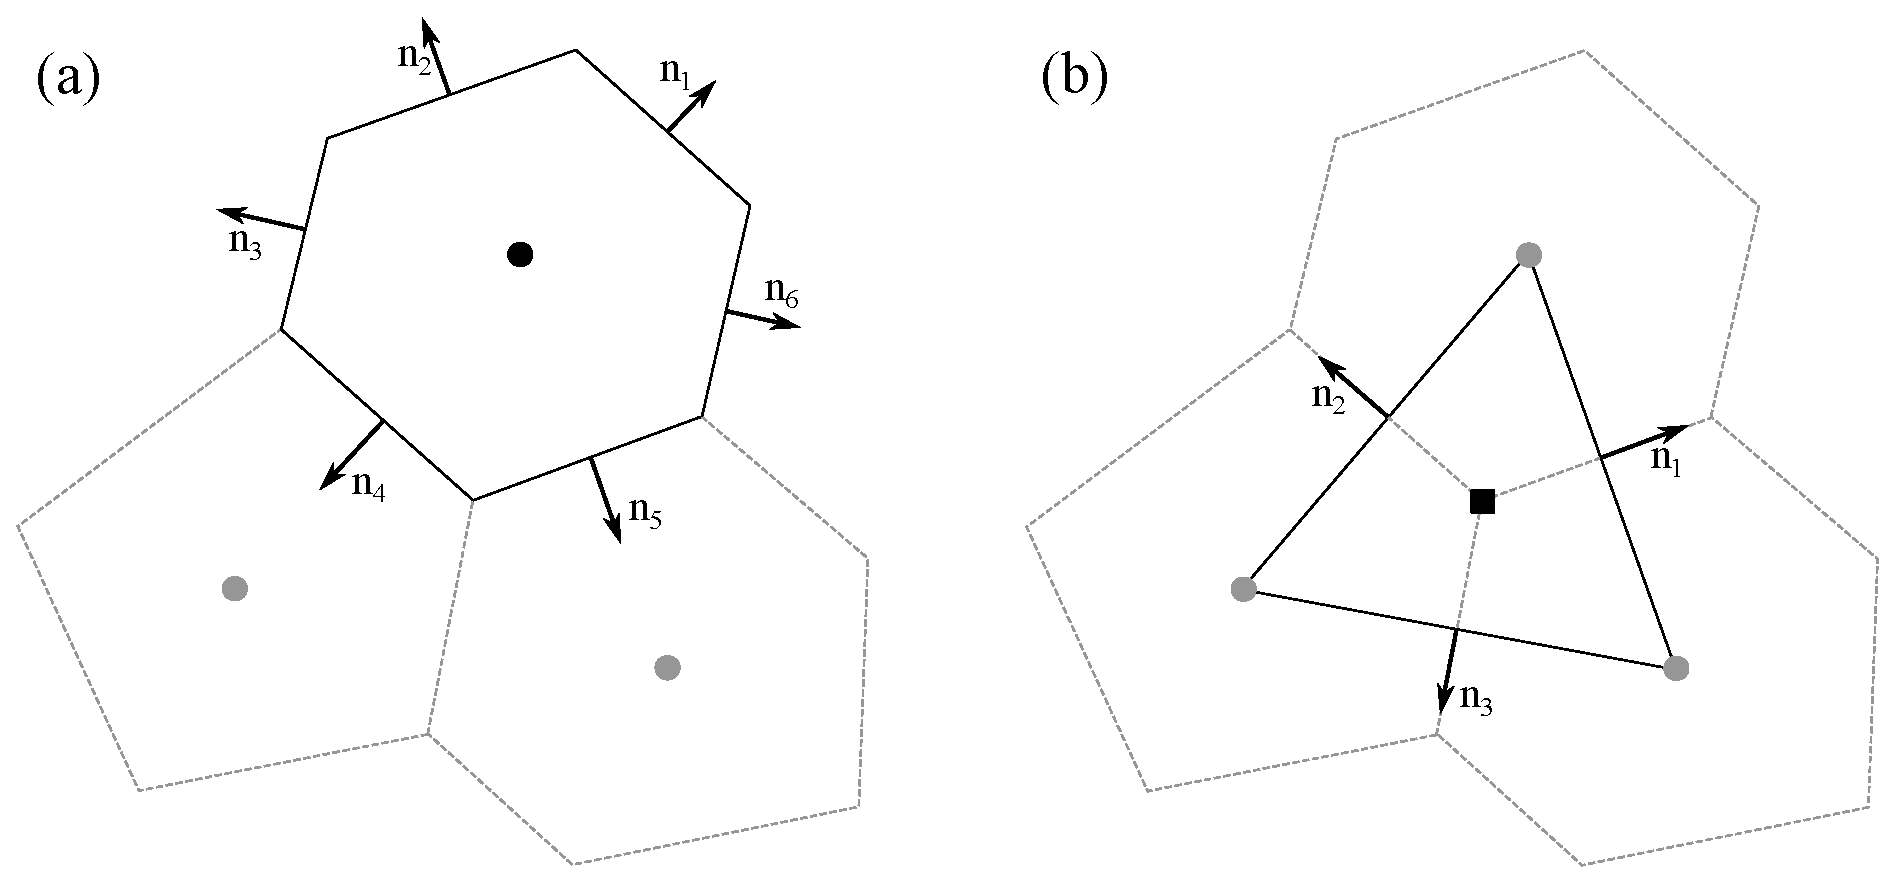
\includegraphics[width=\linewidth]{seaice/figures/mesh_weak.eps}
\caption{Contour integration lines used by the weak scheme. (a): Strain rate at cell centers (\emph{circle}) are calculated from line integrals around primary mesh cells (\emph{solid line}). (b): Divergence of stress at cell vertices (\emph{square}) are calculated from line integrals around the dual mesh cells (\emph{solid line}). Directions of normal vectors used in the integrals are shown for both figures.}
\label{fig:mesh_weak}
\end{figure}

For the weak scheme we use line integrals around cells in the primary and dual meshes to calculate the strain rate tensor and the divergence of stress, respectively. To determine the strain rate tensor we start from the following vector identity:
\begin{equation}
\boldsymbol{\nabla} \cdot (\boldsymbol{u} \otimes \boldsymbol{v}) = (\boldsymbol{u} \cdot \boldsymbol{\nabla}) \boldsymbol{v} + (\boldsymbol{\nabla} \cdot \boldsymbol{u}) \boldsymbol{v}
\label{eqn:vector_identity}
\end{equation}
and from the divergence theorem:
\begin{equation}
\int_\Omega \left[ \boldsymbol{\nabla} \cdot (\boldsymbol{u} \otimes \boldsymbol{v}) \right] \partial{\Omega} = \oint_S \left[\boldsymbol{n} \cdot (\boldsymbol{u} \otimes \boldsymbol{v}) \right] \partial{S} = \oint_S \left[(\boldsymbol{n} \cdot \boldsymbol{u}) \boldsymbol{v} \right] \partial{S}
\label{eqn:divergence_theorem}
\end{equation}
where $\boldsymbol{n}$ is a normal vector to the surface $S$ and $\otimes$ is the tensor product.
If equation \ref{eqn:vector_identity} is integrated over $\Omega$, using equation \ref{eqn:divergence_theorem} we obtain
\begin{equation}
\int_\Omega \left[ (\boldsymbol{u} \cdot \boldsymbol{\nabla}) \boldsymbol{v} + (\boldsymbol{\nabla} \cdot \boldsymbol{u}) \boldsymbol{v} \right] \partial{\Omega} = \oint_S \left[(\boldsymbol{n} \cdot \boldsymbol{u}) \boldsymbol{v} \right] \partial{S}
\label{eqn:weak1}
\end{equation}
If $\boldsymbol{u}$ is chosen as constant then $\boldsymbol{\nabla} \cdot \boldsymbol{u}$ vanishes as does the second term in equation \ref{eqn:weak1}. Taking, also, $\boldsymbol{u}$ sequentially as the cartesian unit vectors spanning $\Omega$ and summing the results we obtain
\begin{equation}
\int_\Omega \left[ \boldsymbol{\nabla} \boldsymbol{v} \right] \partial{\Omega} = \oint_S \left[ \boldsymbol{n} \otimes \boldsymbol{v} \right] \partial{S}
\end{equation}
The symmetric version of this operator is then obtained as:
\begin{equation}
\int_\Omega \left[ \boldsymbol{\nabla_S} \boldsymbol{v} \right] \partial{\Omega} = \oint_S \left[ \boldsymbol{n} \otimes \boldsymbol{v} + \boldsymbol{v} \otimes \boldsymbol{n} \right] \partial{S}
\end{equation}
The strain rate at a point is then obtained from the limit
\begin{equation}
\boldsymbol{\dot{\epsilon}} = \boldsymbol{\nabla}_S \boldsymbol{v} = \lim_{A \to 0} \frac{1}{A} \oint \frac{1}{2}\left[ \boldsymbol{n} \otimes \boldsymbol{v} + \boldsymbol{v} \otimes \boldsymbol{n} \right] \mathrm{d}l
\end{equation}
where the integral is around a closed loop with area $A$ and normal vector $\boldsymbol{n}$, and $\boldsymbol{v}$ is the sea-ice velocity.
To determine the strain rate tensor at the centers of the primary mesh, we take this integration around the edges of the cells in the primary mesh. First the cell is projected onto a flat tangent plane perpendicular to the vector joining the center of the sphere to the cell center. We take the sea ice velocity at a cell edge as the average of the values on the two vertices forming that edge projected onto the tangent plane:
\begin{equation}
\boldsymbol{\dot{\epsilon}}^\prime = \frac{1}{A} \sum_i^{n_e} \frac{1}{2} \left[ \boldsymbol{n}_i \otimes \boldsymbol{v}_i + \boldsymbol{v}_i \otimes \boldsymbol{n}_i \right] l_i
\end{equation}
Here, $A$ is the area of the primary cell, the summation is over the $n_e$ edges of the primary cell, $\boldsymbol{n}_i$ is the normal vector to the edge $i$ that lies in the tangent plane, $\boldsymbol{v}_i$ is the edge velocity and $l_i$ is the length of edge $i$. We use the tangental projection of the velocity and account for metric terms separately. The full strain rate tensor including these metric terms is \citep{Batchelor67}:
\begin{equation}
\dot{\epsilon}_{11} = \dot{\epsilon}_{11}^\prime - \frac{v \tan{\phi}}{r}
\end{equation}
\begin{equation}
\dot{\epsilon}_{22} = \dot{\epsilon}_{22}^\prime
\end{equation}
\begin{equation}
\dot{\epsilon}_{12} = \dot{\epsilon}_{12}^\prime + \frac{u \tan{\phi}}{2r}
\end{equation}
where the prime symbol signifies a strain rate without metric terms.
The stress, which is determined from the strain rate tensor using the constitutive relation, is now defined on cell centers. To find its divergence we use the divergence theorem:
\begin{equation}
\iint \boldsymbol{\nabla} \cdot \boldsymbol{\sigma} \mathrm{d}A = \oint \left[ \boldsymbol{\sigma} \cdot \boldsymbol{n} \right] \mathrm{d}l
\end{equation}
or
\begin{equation}
\boldsymbol{\nabla} \cdot \boldsymbol{\sigma} = \lim_{A \to 0}  \frac{1}{A} \oint \left[ \boldsymbol{\sigma} \cdot \boldsymbol{n} \right] \mathrm{d}l
\end{equation}
for the divergence of stress at a point.
The divergence of internal stress is determined at primary cell vertices (where the velocity is defined and momentum equation solved) by performing a sum around the edges of the dual mesh on a tangent projected plane, tangental to the primary cell vertex. The vertices of the dual mesh are the cell centers of the primary mesh where the strain rate has been determined. The divergence of stress at primary cell vertices is then given by
\begin{equation}
(\boldsymbol{\nabla} \cdot \boldsymbol{\sigma})^\prime = \frac{1}{A_d} \sum_i^{n_c} \left[ \boldsymbol{\sigma}_i \cdot \boldsymbol{n}_i \right] l_i
\end{equation}
where $A_d$ is the area of the dual mesh cell, the sum is over the $n_c$ vertices of the dual mesh, $l_i$ is the length of the $i$ edge of the dual mesh, and $n_i$ is a normal vector to the $i$ edge on the projected plane. As before, this gives a result without taking into account metric effects of the mesh. With those effects the divergence of stress is:
\begin{equation}
(\nabla \cdot \sigma)_u = (\nabla \cdot \sigma)_u^\prime - \frac{2 \sigma_{12} \tan{\phi}}{r}
\end{equation}
\begin{equation}
(\nabla \cdot \sigma)_v = (\nabla \cdot \sigma)_v^\prime + \frac{(\sigma_{11} + \sigma_{22}) \tan{\phi}}{r}
\end{equation}
where the components of $\boldsymbol{\sigma}$ are approximated as the
average of the values on the dual mesh vertices.

\vspace{0.5in}
{\small
\begin{center}
\begin{longtable}{| p{2.0in} || p{4.0in} |}
    \hline
    {\bf Name} & {\bf Description} \endfirsthead
    \hline 
    {\bf Name} & {\bf Description} (Continued) \endhead
    \hline
    \hline
    \hyperref[subsec:nm_sec_config_dynamics_subcycle_number]{config\_dynamics\_subcycle\_numbe-}\hyperref[subsec:nm_sec_config_dynamics_subcycle_number]{r}& {\bf \color{red} MISSING} \\
    \hline
    \hyperref[subsec:nm_sec_config_rotate_cartesian_grid]{config\_rotate\_cartesian\_grid} & {\bf \color{red} MISSING} \\
    \hline
    \hyperref[subsec:nm_sec_config_include_metric_terms]{config\_include\_metric\_terms} & {\bf \color{red} MISSING} \\
    \hline
    \hyperref[subsec:nm_sec_config_elastic_subcycle_number]{config\_elastic\_subcycle\_number} & {\bf \color{red} MISSING} \\
    \hline
    \hyperref[subsec:nm_sec_config_stress_divergence_scheme]{config\_stress\_divergence\_sche-}\hyperref[subsec:nm_sec_config_stress_divergence_scheme]{me}& {\bf \color{red} MISSING} \\
    \hline
    \hyperref[subsec:nm_sec_config_variational_basis]{config\_variational\_basis} & {\bf \color{red} MISSING} \\
    \hline
    \hyperref[subsec:nm_sec_config_wachspress_integration_type]{config\_wachspress\_integration\_-}\hyperref[subsec:nm_sec_config_wachspress_integration_type]{type}& {\bf \color{red} MISSING} \\
    \hline
    \hyperref[subsec:nm_sec_config_wachspress_integration_order]{config\_wachspress\_integration\_-}\hyperref[subsec:nm_sec_config_wachspress_integration_order]{order}& {\bf \color{red} MISSING} \\
    \hline
    \hyperref[subsec:nm_sec_config_revised_evp]{config\_revised\_evp} & {\bf \color{red} MISSING} \\
    \hline
    \hyperref[subsec:nm_sec_config_use_air_stress]{config\_use\_air\_stress} & {\bf \color{red} MISSING} \\
    \hline
    \hyperref[subsec:nm_sec_config_use_ocean_stress]{config\_use\_ocean\_stress} & {\bf \color{red} MISSING} \\
    \hline
    \hyperref[subsec:nm_sec_config_use_surface_tilt]{config\_use\_surface\_tilt} & {\bf \color{red} MISSING} \\
    \hline
    \hyperref[subsec:nm_sec_config_geostrophic_surface_tilt]{config\_geostrophic\_surface\_tilt} & {\bf \color{red} MISSING} \\
    \hline
\end{longtable}
\end{center}
}
\section[advection]{\hyperref[sec:nm_sec_advection]{advection}}
\label{sec:nm_tab_advection}
The advection namelist record controls options assocated with advection of thickness and tracers.  Tracer advection is not currently supported.

\vspace{0.5in}
{\small
\begin{center}
\begin{longtable}{| p{2.0in} || p{4.0in} |}
    \hline
    {\bf Name} & {\bf Description} \endfirsthead
    \hline 
    {\bf Name} & {\bf Description} (Continued) \endhead
    \hline
    \hline
    \hyperref[subsec:nm_sec_config_advection_type]{config\_advection\_type} & Type of advection scheme (upwind or incremental remapping) \\
    \hline
    \hyperref[subsec:nm_sec_config_monotonic]{config\_monotonic} & If true then fluxes are limited to produce a monotonic advection scheme \\
    \hline
    \hyperref[subsec:nm_sec_config_conservation_check]{config\_conservation\_check} & {\bf \color{red} MISSING} \\
    \hline
    \hyperref[subsec:nm_sec_config_monotonicity_check]{config\_monotonicity\_check} & {\bf \color{red} MISSING} \\
    \hline
    \hyperref[subsec:nm_sec_config_recover_tracer_means_check]{config\_recover\_tracer\_means\_check} & {\bf \color{red} MISSING} \\
    \hline
\end{longtable}
\end{center}
}
\section[column\_package]{\hyperref[sec:nm_sec_column_package]{column\_package}}
\label{sec:nm_tab_column_package}
Namelist parameters for the \verb+column_package+ namelist group.

\vspace{0.5in}
{\small
\begin{center}
\begin{longtable}{| p{2.0in} || p{4.0in} |}
    \hline
    {\bf Name} & {\bf Description} \endfirsthead
    \hline 
    {\bf Name} & {\bf Description} (Continued) \endhead
    \hline
    \hline
    \hyperref[subsec:nm_sec_config_use_column_shortwave]{config\_use\_column\_shortwave} & {\bf \color{red} MISSING} \\
    \hline
    \hyperref[subsec:nm_sec_config_use_column_vertical_thermodynamics]{config\_use\_column\_vertical\_ther-}\hyperref[subsec:nm_sec_config_use_column_vertical_thermodynamics]{modynamics}& {\bf \color{red} MISSING} \\
    \hline
    \hyperref[subsec:nm_sec_config_use_column_biogeochemistry]{config\_use\_column\_biogeochemist-}\hyperref[subsec:nm_sec_config_use_column_biogeochemistry]{ry}& {\bf \color{red} MISSING} \\
    \hline
    \hyperref[subsec:nm_sec_config_use_column_itd_thermodynamics]{config\_use\_column\_itd\_thermody-}\hyperref[subsec:nm_sec_config_use_column_itd_thermodynamics]{namics}& {\bf \color{red} MISSING} \\
    \hline
    \hyperref[subsec:nm_sec_config_use_column_ridging]{config\_use\_column\_ridging} & {\bf \color{red} MISSING} \\
    \hline
\end{longtable}
\end{center}
}
\section[column\_tracers]{\hyperref[sec:nm_sec_column_tracers]{column\_tracers}}
\label{sec:nm_tab_column_tracers}
Namelist parameters for the \verb+column_tracers+ namelist group.

\vspace{0.5in}
{\small
\begin{center}
\begin{longtable}{| p{2.0in} || p{4.0in} |}
    \hline
    {\bf Name} & {\bf Description} \endfirsthead
    \hline 
    {\bf Name} & {\bf Description} (Continued) \endhead
    \hline
    \hline
    \hyperref[subsec:nm_sec_config_use_ice_age]{config\_use\_ice\_age} & {\bf \color{red} MISSING} \\
    \hline
    \hyperref[subsec:nm_sec_config_use_first_year_ice]{config\_use\_first\_year\_ice} & {\bf \color{red} MISSING} \\
    \hline
    \hyperref[subsec:nm_sec_config_use_level_ice]{config\_use\_level\_ice} & {\bf \color{red} MISSING} \\
    \hline
    \hyperref[subsec:nm_sec_config_use_cesm_meltponds]{config\_use\_cesm\_meltponds} & {\bf \color{red} MISSING} \\
    \hline
    \hyperref[subsec:nm_sec_config_use_level_meltponds]{config\_use\_level\_meltponds} & {\bf \color{red} MISSING} \\
    \hline
    \hyperref[subsec:nm_sec_config_use_topo_meltponds]{config\_use\_topo\_meltponds} & {\bf \color{red} MISSING} \\
    \hline
    \hyperref[subsec:nm_sec_config_use_aerosols]{config\_use\_aerosols} & {\bf \color{red} MISSING} \\
    \hline
\end{longtable}
\end{center}
}
\section[biogeochemistry]{\hyperref[sec:nm_sec_biogeochemistry]{biogeochemistry}}
\label{sec:nm_tab_biogeochemistry}
\section{Biogeochemistry}
\label{sec:biogeochemistry}

% 
\newcommand\bgcNO{\mbox{NO$_3$}}
\newcommand\bgcNH{\mbox{NH$_4$}}
\newcommand\bgcSi{\mbox{SiO$_3$}}
\newcommand\bgcN{\mbox{N}}
\newcommand\bgcDOC{\mbox{DOC}}
\newcommand\bgcDON{\mbox{DON}}
\newcommand\bgcfed{\mbox{fed}}
\newcommand\bgcfep{\mbox{fep}}
\newcommand\bgcchl{\ensuremath{\mbox{Chl}a}}
\newcommand\bgcDMS{\mbox{DMS}}
\newcommand\bgcDMSP{\mbox{DMSP}}
\newcommand\bgcDMSPp{\mbox{DMSPp}}
\newcommand\bgcDMSPd{\mbox{DMSPd}}
\newcommand\bgcPON{\mbox{PON}}
\newcommand\zaeroBC{\mbox{BC}}
\newcommand\zaerodust{\mbox{dust}}
\newcommand\bgcie{i.e.\ }


There are two options for modeling  biogeochemistry in  sea ice: 1) a
skeletal layer or bottom layer model (skl-model) that assumes
biology and biogeochemical molecules are restricted to a single layer at the base of the sea ice;
and 2) a vertically resolved model (zbgc) that allows for biogeochemical processes throughout the
ice column.  The two models may be run with the same suite of
biogeochemical tracers and use the same set of nonlinear coupled equations to determine the biochemical
reaction terms for the tracers at each vertical grid level.  In the
case of the skeletal layer model this is a single layer, while for
zbgc  there are {\tt nBioLayers}$+1$ vertical layers.  The primary difference between the
two schemes is in the vertical transport assumptions for each
biogeochemical tracer.  This includes the parameterizations
of fluxes between ocean and ice.  

For both models, there are configuration variables that, in part, specify the
complexity of the ecosystem.  In Registry.xml these are 1) {\tt nAlgae}, the number of algal species; 2)
{\tt nDOC}, the number of dissolved organic carbon groups, 3)  {\tt
  nDIC}, the number of dissolved inorganic carbon groups, 4)
{\tt nDON}, the number of dissolved organic nitrogen groups, 5)  {\tt
  nParticulateIron}, the number of particulate iron groups; and 6) {\tt nDissolvedIron},
the number of dissolved iron groups.  The current version of the
 biochemistry has parameters for up to 3 algal
species (diatoms, small phytoplankton and {\it Phaeocystis} sp,
respectively), 2 dissolved organic carbon (DOC) tracers (polysaccharids and lipids,
respectively), 0 dissolved inorganic carbon (DIC) tracers, 1 dissolved
organic nitrogen (DON) tracer (proteins/amino acids),
1 particulate iron tracer and 1 dissolved iron tracer.  However the
carbon, DOC and DIC, tracers are not fully implented in this version and
should not be used out of the box. Note also that for
tracers with multiple species/groups, the
order is important.  For example, specifiying {\tt nALG}$ = 1$ will
compute reaction terms using parameters specific to ice diatoms.  

In addition to specifying the group size, individual biogeochemical
tracer groups must also be set as true in namelist.cice.
These includes the nutrients: nitrate (config\_use\_nitrate), silicate
(config\_use\_silicate), ammonium (config\_use\_ammonium), and
dissolved iron (config\_use\_iron);  the dimethylsulphide group: DMS, DMSPp,
DMSPd (config\_use\_DMS); carbon: DOC and DIC (config\_use\_carbon);
DON (config\_use\_DON);
humic material (config\_use\_humics); a non-adsorptive passive tracer
(config\_use\_nonreactive); and particulate and dissolved iron (config\_use\_iron). 

Biogeochemical upper ocean concentrations are initialized in the
subroutine \newline {\bf colpkg\_init\_ocean\_conc}
in {\bf ice\_colpkg.F90} using a default set of fixed values unless
coupled to the ocean biogeochemistry. In coupled ice-ocean
biogeochemical simulations, ocean surface concentrations for diatoms,
small plankton, {\it Phaeocystis} sp, nitrate, silicate, ammonium, and
dissolved iron are passed to the sea ice biogeochemistry.  The sea ice
computes return fluxes based on the local brine fluxes, and/or ice growth
and melt rates. 

\subsection{Skeletal Layer BGC}

In the skeletal layer model, ice algal biogeochemistry is modelled as a single layer
of reactive tracers attached to the sea ice bottom. This assumption
has greater validity in the Arctic than in the Southern Ocean where internal
and freeboard communitites are common.
To use skl-bgc, set the following namelist.cice configuration options
to true: {\tt config\_use\_brine}, \newline {\tt config\_use\_column\_biogeochemistry},
{\tt config\_use\_skeletal\_biochemistry}.

Skeletal tracers ($T_{b}$) are ice area ($a_{i}$) conserved
and, for each thickness category $n$, satisfy the horizontal transport equation: 
\begin{eqnarray}
\label{eqn:bgc_tracer_thickness_cons}
\frac{\partial (T_{bn} a_{in})}{\partial t} + \Delta \cdot (T_{bn} a_{in} {\bf u}) & = & 0
\end{eqnarray}
for horizontal velocity {\bf u}.

In addition, the column biogeochemistry solves a coupled set of reaction equations which define transformations between biogeochemical tracers and computes fluxes between the ice and ocean:
\begin{eqnarray}
\label{eqn:bgc_Tracer}
\frac{\partial T_b}{\partial t}  & = & w_b \frac{\Delta T_b}{\Delta z} +  R_b({T_j : j = 1,\ldots,N_b})
\end{eqnarray}
where $R_b$ represents the nonlinear biochemical reaction terms
(described in section~\ref{sec:reactions})
 and $\Delta z$ is a length scale
representing the molecular sublayer of the ice-ocean interface.  Its
value is absorbed in the piston velocity parameters.  The piston
velocity $w_b$  depends
on the particular tracer and the flux formulation.  There are two types of ice-ocean tracer flux formulations: 1)
`Jin2006' modelled after the growth rate dependent piston velocity of \cite{Jin:sklbgc:2006}
and 2) `constant' which sets the piston velocity to a constant (\cite{Elliott:sklbgc:2012}).
The formulation is chosen in  {\bf namelist.seaice} by setting {\tt config\_skeletal\_bgc\_flux\_type} equal to
`Jin2006' or `constant'. 

The default parameterization,  `Jin2006', assumes the piston velocity is a function of ice growth and melt rates.  All tracers (algae included) flux with the same piston velocity during ice thickness growth,
 $dh_i/dt > 0$:
\begin{eqnarray}
\label{eqn:pwJin_growth}
w_b  & =  & - p_g\left|m_1 + m_2 \frac{dh_i}{dt} - m_3
  \left(\frac{dh_i}{dt} \right)^2\right|
\end{eqnarray}
with parameters $m_1$, $m_2$, $m_3$ and $p_g$ defined
in {\bf skl\_biogeochemistry} in {\bf ice\_algae.F90}. 
For ice melt, $dh_i/dt < 0$, all tracers with the exception of ice algae
flux with 
\begin{eqnarray}
\label{eqn:pwJin_melt}
w_b  & =  & p_m\left|m_2 \frac{dh}{dt} - m_3
    \left(\frac{dh}{dt}  \right)^2\right| 
\end{eqnarray}
with $p_m$ defined
in {\bf skl\_biogeochemistry}. 
The `Jin2006' formulation also requires that for both expressions, $|w_b| \leq 0.9
h_{sk}/\Delta t$ where $h_{sk}=0.03\,m$ is the skeletal layer thickness.  
The concentration difference at the ice-ocean boundary for each tracer, $\Delta
T_b$, depends on the sign of $w_b$.  For growing ice, $w_b < 0$,
$\Delta T_b  = T_b/h_{sk} - T_{io}$, where $T_{io}$ is the ocean
concentration of tracer $i$. For melting
ice,  $w_b > 0$, $\Delta T_b = T_b/h_{sk}$.

In  `Jin2006', the algal tracer ($N_a$) responds to ice melt in the same manner as
the other tracers (\ref{eqn:pwJin_melt}).  However, during ice growth, the skeletal algal concentration remains fixed unless the ice algal brine concentration is less than the ocean algal concentration ($N_o$).  In this case, the ocean seeds the sea ice according to  
\begin{eqnarray}
\label{eqn:seed}
w_b \frac{\Delta N_a}{\Delta z} & = & \frac{N_oh_{sk}/\phi_{sk} -
  N_a}{\Delta t}
\end{eqnarray}
where $\phi_{sk}=0.3$ is the skeletal layer porosity.

The `constant' formulation uses a fixed piston velocity for positive ice growth rates for all tracers except $N_a$.  As
in `Jin2006', congelation ice growth seeds the sea ice algal
population according to (\ref{eqn:seed}) when $N_a < N_o
h_{sk}/\phi_{sk}$. For bottom ice melt, all tracers follow the prescription
\begin{eqnarray} 
 w_b \frac{\Delta T_b}{\Delta z} & = &  \left\{ \begin{array}{ll}
   T_b   |dh_i/dt|/h_{sk} \ \ \ \ \ &   \mbox{if }
 |dh_i/dt|\Delta t/h_{sk} < 1  \\
 T_b/\Delta t & \mbox{otherwise.}   \end{array} \right.  
\label{eqn:constant_melt}
\end{eqnarray}

A detailed description of the biogeochemistry reaction terms is given
in section~\ref{sec:reactions}. 

\subsection{Vertical ``Z'' BGC}
\label{sec:zbgc}
In order to solve the vertically resolved biogeochemistry, set the
following configuration options in {\bf namelist.cice} to true: a)
{\tt config\_use\_brine}, b) {\tt config\_use\_vertical\_tracers}, and
\newline c) {\tt
  config\_use\_vertical\_biochemistry}.
\begin{itemize}
\item a) {\tt config\_use\_brine} true, turns on the dynamic brine
  fraction tracer, $f_b$, (see section~\ref{sec:brine}) which defines the vertical domain of the
  biogeochemical tracers .  z-Tracer horizontal transport is conserved on ice
  volume$\times$brine height fraction.
\item b) {\tt config\_use\_vertical\_tracers} true, indicates use of vertically resolved
  biogeochemical and z-aerosol tracers.  This flag alone turns on the
  vertical transport scheme but not the biochemistry.
\item c) {\tt config\_use\_vertical\_biochemistry} true, turns on the biochemistry for the
  vertically resolved tracers and automatically turns on the algal
  nitrogen. If false, algal nitrogen is not transported and any other biogeochemical tracers in use is
  transported as a passive tracer.  This is appropriate for the black
  carbon and dust aerosols specified by {\tt config\_use\_zaerosols} true.
\end{itemize}
In addition, a halodynamics scheme must also be on.  The default
thermo-halodynamics is mushy layer {\tt config\_thermodynamics\_type} set to 2.  An
alternative uses \cite{Bitz:thermo:1999}'s thermodynamics ({\tt config\_thermodynamics\_type} set
to 1) and {\tt config\_use\_vertical\_salinity} true (referred to as ``zsalinity''). 

Vertically resolved z-tracer bulk concentrations ($T_{zb}$) are  brine volume fraction conserved and thus
depend on both the ice volume ($v_{i}$) and the brine height fraction tracer ($f_b$).   These tracers follow the conservation equations for multiply dependent
tracers:
\begin{eqnarray}
\label{eqn:zbgc_tracer_thickness_cons}
\frac{\partial (T_{zbn} v_{in}f_{bn})}{\partial t} + \Delta \cdot (T_{zbn} v_{in}f_{bn} {\bf u}) & = & 0.
\end{eqnarray}

The following sections describe the vertical biological grid, the
vertical transport equation for mobile tracers, the partitioning of
tracers into  mobile and stationary fractions and the
biochemical reaction equations.
\subsection{Bio grid}
\label{sec:bio_grid}
The bio grid  is a vertical grid used for solving the brine height
variable ($h_b = f_b h_i$) and descretizing the vertical transport equations of
biogeochemical tracers. The grid is non-dimensional and takes the value zero at the brine surface and one at the ice-ocean
interface.  The number of grid levels is specified during Registry.xml  by setting the variable {\tt nBioLayers}
integer ($n_b$) .  

Ice tracers and microstructural properties defined on the bio grid are
 referenced in two ways: as
1)  $n_b+2$ {\tt bgrid} points  and 2) $n_b+1$ {\tt igrid} points.
For both  {\tt bgrid} and {\tt igrid}, the first and last points reference
the brine surface and the ice-ocean interface and so take the values $0$ and $1$,
respectively.  For  {\tt bgrid}, the interior points $[2, n_b+1]$ are
spaced at $1/n_b$ intervals beginning with {\tt bgrid(2)}$ =
1/(2n_b)$.  The {\tt igrid} interior points $[2, n_b]$ are also
equidistant with the same spacing, but physically coincide  with
points midway between those of the {\tt bgrid}.

 \subsubsection{Transport along the interface bio grid}  

Purely mobile biogeochemical tracers are tracers which move with the brine and thus,
in the absence of biochemical reactions, evolve in a manner like salinity.  In the vertical tracer transport of purely mobile tracers, the flux conserved quantity is the bulk
tracer concentration multiplied by the ice thickness, \bgcie $C = h\phi
[c]$, where $h$ is the ice thickness, $\phi$ is the porosity, and
$[c]$ is the tracer concentration in the brine.  $\phi$, $[c]$ and $C$  are defined on the interface bio grid (igrid):
\begin{eqnarray}
\mbox{igrid}(k) & =  & \Delta (k-1) \ \ \ \mbox{for }k = 1:n_b+1
\end{eqnarray}
and $\Delta = 1/n_b$

The biogeochemical module solves the equation:
\begin{eqnarray}
\frac{\partial C}{\partial t} & =& \frac{\partial }{\partial x}\left\{
\left( \frac{v}{h} + \frac{w_f}{h\phi} -
  \frac{\tilde{D}}{h^2\phi^2}\frac{\partial \phi}{\partial x} \right) C
+ \frac{\tilde{D}}{h^2\phi}\frac{\partial C}{\partial x} 
\right\} + h\phi R([c]) \label{eqn:mobile_transport}
\end{eqnarray}
where $D_{in} = \tilde{D}/h^2 =  (D + \phi D_m)/h^2$ (\cite{Jeffery:tracers:2011})
and $R([c])$ is
the nonlinear biogeochemical interaction term.

Solutions to (\ref{eqn:mobile_transport}) are found using a flux-corrected and
positive definite finite element
Gelerkin discretization.  Details are in section~\ref{append:tracer_numerics}.

\subsection{Splitting tracers:  config\_mobility\_type}
In addition to purely mobile tracers such as nitrate, some biogeochemical tracers also adsorb or
otherwise adhere to the ice crystals.  These tracers exist in both the
mobile and stationary phasea and their  
total brine concentration is a sum $c_m + c_s$
where $c_m$ is the moble fraction transported by
(\ref{eqn:mobile_transport}) and $c_s$  remains vertically fixed during ice growth/melt and brine motion.  The primary algal group, discussed below,  are a notable exception.  

In order to model the transfer between these fractions, we assume that tracers adhere to the crystals with a time-constant of
$\tau_{ret}$, and release with a time constant $\tau_{rel}$, \bgcie
\begin{eqnarray}
\frac{\partial c_m}{\partial t} & = & -\frac{c_m}{\tau_{ret}} + \frac{c_s}{\tau_{rel}} \\
\nonumber
\frac{\partial c_s}{\partial t} & = &\frac{c_m}{\tau_{ret}} - \frac{c_s}{\tau_{rel}}
\end{eqnarray}
 
We use the exponential form of these equations:
\begin{eqnarray}
c_m^{t+dt} & = &
c_m^t\exp\left(\left\{-\frac{dt}{\tau_{ret}}\right)\right\} +
c^t_s\left(1- \exp\left[-\left\{\frac{dt}{\tau_{rel}}\right\}\right]\right)  \nonumber
\end{eqnarray}
\begin{eqnarray}
c_s^{t+dt} & = & c_s^t\exp\left(\left\{-\frac{dt}{\tau_{rel}}\right)\right\} +
c_m^t\left(1-\exp\left[-\left\{\frac{dt}{\tau_{ret}}\right\}\right]\right) \nonumber
\end{eqnarray}
The time constants are functions of the ice growth and melt rates
($dh/dt$). All tracers except algal nitrogen diatoms follow the 
simple case: when $dh/dt \geq 0$, then $\tau_{rel} \rightarrow \infty$ and
$\tau_{ret}$ is finite.  For $dh/dt < 0$, then $\tau_{ret} \rightarrow \infty$ and
$\tau_{rel}$ is finite.  In other words,  ice growth promotes transitions to the
stationary phase and ice melt enables transitions to the mobile phase.

The adsorption of tracers is also bound by a saturation concentration which is determined from geometric properties of the ice crystals (assumed to be spheres), and the size and shape of the adsorbing particle (prolate spheroids)  (\cite{Johnson:bac:1995}).  When the stationary concentration reaches or exceeds the saturation concentration, adsorption stops and the additional material remains in the mobile phase.

Diatoms are somewhat unique in that they have the ability to move independently. Although we do not model motility in an advective sense, we assume that diatoms, the first
algal nitrogen group, actively maintain their
relative position within the ice, \bgcie bottom (interior, upper) algae
remain in the bottom (interior, upper) ice, unless melt rates exceed a
threshold.  The configuration parameter {\tt config\_algal\_maximum\_velocity} sets this
threshold. 

\subsection{Mobile and Stationary Phases}
\label{sec:mobile_and_stationary}
There are 5 possible mobility types indicated by the set $\{-1, 0,
0.5, 1, 2\}$ which assigns a combination of a fast and slow timescale
to the release and retention of tracers.  In {\bf namelist.cice}, the
parameters beginning {\tt config\_mobility\_type\_} specify the
vertical transport behavior of each biogeochemical in the code and
{\tt config\_long\_mobile\_to\_stationary\_time} and \newline
{\tt config\_rapid\_mobile\_to\_stationary\_time} define the maximum (slow) and minimum (fast)  timescales (rates).  For a mobility type of -1, the tracer remains solely in the mobile
phase throughout the simulation.  This is the default for nitrate and silicate.  For mobility types of 0, the tracer has maximal rates (\bgcie minimum timescale) of retention and slow rates (\bgcie maximum timescale) of release back to the mobile phase.  For a value of 1, the tracer has slow rates in
the retention phase and fast release to mobility.  For a mobility type of 0.5, 
minimum timescales are used for both
transitions, and for a value of 2, maximal timescales are used. Table~\ref{table:phases} summarizes the transition types.

\begin{table}[t!]
\caption{Types of Mobile and Stationary Transitions}
\begin{tabular}{l|l|l|l} \hline 
{\bf{config\_mobility\_type}} &$ \tau_{ret}$ & $\tau_{rel}$ & Description \\ \hline 
-1  & $\infty$ & 0 & entirely in the mobile phase \\
0   & min & max & retention dominated \\
1   & max & min & release dominated \\
0.5   & min & min & equal but rapid exchange \\
2  & max & max & equal but slow exchange \\
\hline
\end{tabular}\label{table:phases}
\end{table}

The fraction of a given tracer in the mobile phase is independent of
ice depth and stored in the
tracer variable  {\tt zbgc\_frac}. The horizontal transport of this
tracer is conserved on brine volume fraction and so is dependent on two
tracers: brine height fraction ($f_b$) and ice volume ($v_{in}$) (\ref{eqn:zbgc_tracer_thickness_cons}).  The tracer, {\tt zbgc\_frac}, is initialized to 1 during new ice formation because
 all z-tracers are assumed to be initially in the purely mobile phase.
As the ice melts, z-tracers return to the mobile phase.
Very large release timescales will prevent this transition and could
result in an unphysically large accumulation during the melt season.

\subsection{Brine Fraction Tracer} 
\label{sec:brine} 
\index{brine}
The brine height, $h_b$, is the distance from the
ice-ocean interface to the brine surface. It is the vertical domain
for all ice biogeochemical tracers and aerosols.   When {\tt
  config\_use\_brine} is set true in {\bf namelist.cice} the position
of the  brine
surface  relative moves relative to the
 ice surface. Physically, this occurs when the ice is permeable and there is
a nonzero pressure head: the difference between the brine
height and the equilibrium sea surface. Brine height motion is
computed in {\bf ice\_brine.F90} from thermodynamic variables and the ice microstructural state
deduced from internal bulk salinities and temperature.  This tracer
is required for the transport of vertically resolved biogeochemical
tracers. 
 
Vertical transport
processes are, generally, a result of the brine motion. Therefore the vertical
transport equations for biogeochemical tracers will be defined only
where brine is present.  This region, from the ice-ocean interface to
the brine height, defines the domain of the vertical bio-grid (section~\ref{sec:bio_grid}). The ice
microstructural state, determined in {\bf ice\_brine.F90}, is computed
from sea ice salinities and temperatures linearly interpolated to the
bio-grid.  When $h_b > h_i$, the upper surface brine is assumed to
have the same temperature as the ice surface. 

Brine height is  transported horizontally as the
fraction $f_{b} = h_b/h_i$, a volume conserved
tracer.  Note
that unlike the sea ice porosity, brine height fraction may be greater than 1
when $h_b > h_i$. 

Changes to $h_b$ occur from ice and snow melt, ice
bottom boundary changes,
and from  pressure adjustments. The computation of $h_b$ at $t+\Delta
t$ is a two step process. First,  $h_b$  is updated from
changes in ice and snow thickness ($h_s$), \bgcie
\begin{eqnarray}
\label{eqn:hb_thickness_changes}
h_b' & = & h_b(t) + \Delta h_b|_{h_i,h_s} \ \ \ .
\end{eqnarray}
 Second,  pressure driven adjustments arising from
meltwater flushing and snow loading are applied to $h'_b$. Brine flow due
to pressure forces are governed by
Darcy's equation:
\begin{eqnarray}
\label{eqn:Darcy}
w & = & -\frac{\Pi^* \bar{\rho} g}{\mu}\frac{h_p}{h_i}.  
\end{eqnarray}
where $\mu$ is the viscosity and $g$ is the gravitational acceleration.
The vertical component of the net permeability tensor $\Pi^*$
is computed as
\begin{eqnarray}
\label{eqn:netPi}
\Pi^* & = & \left(\frac{1}{h}\sum_{i=1}^N{\frac{\Delta
      z_i}{\Pi_i}}\right)^{-1} 
\end{eqnarray}
where the sea ice is composed of $N$ vertical layers with $i$th layer
thickness $\Delta z_i$ and
permeability $\Pi_i$. % (\ref{eq:topo_permea}).  
The average sea ice density is
$\bar{\rho}$.
 The hydraulic head is $h_p = h_b - h_{sl}$ where $h_{sl}$ is the sea
 level given by
\begin{eqnarray}
h_{sl} & = & \frac{\bar{\rho}}{\rho_w}h_i + \frac{\rho_s}{\rho_w}h_s \ \ .
\end{eqnarray}
where $\rho_s$ is the snow density and $\rho_w$ is the density of water.
Assuming constant $h_i$ and $h_s$ during Darcy flow, the rate of change of $h_b$ is
\begin{eqnarray}
\label{eqn:h_p}
\frac{\partial h_b}{\partial t}  & = & -w h_p
\end{eqnarray}
where   $w_o = \Pi^* \bar{\rho}
g/(h_i\mu\phi_{top})$ and $\phi_{top}$ is the upper surface porosity. 
When the Darcy flow is downward into the ice ($w_o < 0$), the
$\phi_{top}$ equals the sea ice porosity in the uppermost layer.  However,
when the flow is upwards into the snow, then $\phi_{top}$ equals the snow
porosity {\tt phi\_snow} specified in the namelist {\tt config\_snow\_porosity\_at\_ice\_surface}.  If a negative
number is specified, then the default value is
used: {\tt phi\_snow} $=1 - \rho_s/\rho_w$.

Since $h_{sl}$ remains relatively unchanged during Darcy flow,
(\ref{eqn:h_p}) has the approximate solution 
\begin{eqnarray}
\label{eqn:brine_height}
h_b(t+\Delta t) \approx h_{sl}(t+\Delta t) +  [h'_b - h_{sl}(t+\Delta t)]\exp\left\{-w \Delta t\right\}.
\end{eqnarray}

The contribution $\Delta h_b|_{h_i,h_s}$ arises from snow and ice
melt and bottom ice changes.  Since the ice and brine bottom
boundaries coincide, changes in the ice bottom from growth or melt,
$(\Delta h_i)_{bot}$, equal the bottom brine boundary changes.  The surface
contribution from ice and snow melt, however, is opposite in
sign. The ice contribution is as follows. If $h_i > h_b$ and the ice
surface is melting, ie. $(\Delta h_i)_{top} <
0$), then meltwater increases the brine height:
\begin{eqnarray}
\left(\Delta h_b\right)_{top} & = &  \frac{\rho_i}{\rho_o} \cdot \left\{ \begin{array}{ll}
 -(\Delta h_i)_{top} &  \mbox{if }
 |(\Delta h_i)_{top}| < h_i-h_b  \\
 h_i-h_b & \mbox{otherwise.}   \end{array} \right.  
\end{eqnarray}
For snow melt ($\Delta h_s < 0$), it is assumed that
all snow meltwater contributes a source of surface
brine. The total change from snow melt and ice thickness changes is
\begin{eqnarray}
\label{eqn:dzdt_meltwater}
\Delta h_b|_{h_i,h_s} & = & \left( \Delta
h_b\right)_{top} -\left(\Delta h_i\right)_{bot} -\frac{\rho_s}{\rho_o}\Delta h_s.  
\end{eqnarray}

The above brine height calculation is used only when $h_i$ and $h_b$
exceed a minimum thickness, {\tt thinS}, specified in {\bf
  ice\_zbgc\_shared}. Otherwise 
\begin{eqnarray}
\label{eqn:thinbrine}
h_b(t+\Delta t) & = & h_b(t) + \Delta h_i 
\end{eqnarray}
provided that $|h_{sl}-h_b| \leq 0.001$.  This
formulation ensures small Darcy velocities\index{Darcy flow}
 when $h_b$ first exceeds {\tt thinS}.  
\index{brine}

\subsection{Default Aerosols}

\index{aerosols}Aerosols deposited on the ice gradually
work their way through until the ice melts and they are passed
into the ocean.   They are defined as ice and snow volume tracers, with the
%(Eq.~\ref{eq:transport_viT}  and \ref{eq:transport_vsT}), with the
snow and ice each having two  tracers for each aerosol species, one in
the surface scattering layer (delta-Eddington SSL) and one in the snow or ice interior below the SSL.  

Rather than updating aerosols for each change to ice/snow thickness
due to evaporation, melting,  snow-ice formation, etc., during the
thermodynamics calculation, these  changes are deduced from the
ice diagnostic variables  ({\tt melts, meltb, snoice,} etc) in {\bf
  ice\_aerosol.F90}.   Three processes change the volume of ice or
snow but do not change the  total amount of aerosol, thus causing the
aerosol concentration  (the value of the tracer itself) to change:
evaporation, snow deposition  and basal ice growth.  Basal and lateral
melting remove all  aerosols in the melted portion.  Surface ice and
snow melt leave a  significant fraction of the aerosols behind, but
they do scavenge some fraction given by the parameter  {\tt
  kscav} = [0.03, 0.2, 0.02, 0.02, 0.01, 0.01].   Scavenging also applies
to snow-ice formation.   When sea ice ridges, a fraction of the snow
on the ridging ice is  thrown into the ocean, and any aerosols in that
fraction are also  lost to the ocean.

As upper SSL or interior layers disappear from the snow or ice,
aerosols are transferred to the  next lower layer, or into the ocean
when no ice remains.   The atmospheric flux {\tt faero\_atm} contains
the rates of aerosol  deposition for each species, while {\tt
  faero\_ocn} has the rate at  which the aerosols are transferred to the ocean.

The aerosol tracer flag {\tt config\_use\_aerosols} must be set to true in {\bf
  namelist.cice}, and the number  of aerosol species, {\tt nAerosols}, is set in {\bf
  Registry.xml}.  The following output variables may be added to {\tt
  streams.cice}: {\tt snowScatteringAerosol}, {\tt snowBodyAerosol},
{\tt iceScatteringAerosol}, and {\tt iceBodyAerosol}. 

\subsection{Z-Aerosols}

\index{zaerosols}MPAS-seaice  offers an alternate scheme for aerosols
in sea ice using the brine motion based transport scheme of the
biogeochemical tracers.   All vertically resolved biogeochemical
tracers (z-tracers), including
zaerosols, have the potential to be atmospherically deposited onto the
snow or ice, scavenged during snow melt, and passed into the brine.
The mobile fraction (section~\ref{sec:mobile_and_stationary}) is then transported via brine drainage processes
(\ref{eqn:mobile_transport})
while a stationary fraction (section~\ref{sec:mobile_and_stationary}) adheres
to the ice crystals.  Snow deposition and the process of
scavenging aerosols during snow melt is consistent with the default
aerosol scheme, though parameters have been generalized to accomodate
potential atmospheric deposition for all z-tracers.  For an example,
see the scavenging parameter {\tt kscavz} for z-tracers defined in {\bf
  ice\_zbgc\_shared}.

Within the snow,  z-tracers are defined as concentrations in the snow
surface layer ($h_{ssl}$) and the snow interior ($h_s-h_{ssl}$).  The
total snow content of z-tracers per ice area per grid cell area, $C_{snow}$  is 
\begin{eqnarray}
C_{snow} & = & C_{ssl}h_{ssl} + C_{sint}(h_{s}-h_{ssl}) 
\end{eqnarray}

One major difference in how the two schemes model snow aerosol transport is
that the fraction scavenged from snow melt in the z-tracer scheme is not immediately fluxed
into the ocean, but rather, enters the ice as a source of low
salinity but potentially tracer rich brine.  The snow melt source is
included as a surface flux condition in {\bf ice\_algae.F90}.  

All the z-aerosols are nonreactive with the exception of the
dust aerosols. We assume that a small fraction of the dust flux into
the ice has soluble iron  which is passed to the dissolved iron
tracer (see {\tt config\_solubility\_of\_Fe\_in\_dust} and {\tt
  config\_ratio\_Fe\_to\_dust} in {\bf namelist.cice}).  The remaining dust passes through the ice without reactions.

To use z-aerosols, set {\tt config\_use\_zaerosols}  to true in {\bf
 namelist.cice} and choose up to 6  z-aerosol species {\tt
  nAerosols} in  {\bf
  Registry.xml}.    Note, the default tracers {\tt
  config\_use\_aerosols} must be false. In addition, {\tt
  config\_use\_brine} and {\tt config\_use\_vertical\_tracers} z-tracers and the brine height tracer  must also be
true.   In addition, to turn on the radiative
coupling between the aerosols and the Delta-Eddington radiative
scheme, {\tt config\_shortwave\_type} must equal dEdd and {\tt config\_use\_shortwave\_bioabsorption} must
be true.

\subsection{Biogeochemical Reactions}
\label{sec:reactions}
The biogeochemical reaction terms for each biogeochemical tracer (see
table~\ref{table:bio_tracers} for tracer definitions) are defined in {\bf ice\_algae.F90}
in the subroutine {\tt algal\_dyn}. The same set of equations is used
for the bottom layer  model (when {\tt config\_use\_skeletal\_biochemistry} is true) and the
multi-layer biogeochemical model (when {\tt
  config\_use\_vertical\_biochemistry} and \newline {\tt
  config\_use\_vertical\_tracers} are true).  

\begin{table}[t!]
\caption{Biogeochemical Tracers}    
\begin{threeparttable}
\begin{tabular}{l|l|l|l|l} \hline %  doesn't change lapidus constants
Text Variable & Variable in code & flag config\_use\_ & Description & units \\ \hline
\bgcN(1) &Nin(1) &  {\tt vertical\_biochemistry}$^{c}$ & diatom  & mmol $N/m^3$\\
\bgcN(2) &Nin(2) &  {\tt vertical\_biochemistry}$^{c}$ & small phytoplankton & mmol $N/m^3$\\
\bgcN(3) &Nin(3) &  {\tt vertical\_biochemistry}$^{c}$ & {\it Phaeocystis sp} & mmol $N/m^3$ \\
\bgcDOC(1) &DOCin(1) & {\tt carbon} & polysaccharids & mmol $C/m^3$ \\
\bgcDOC(2) &DOCin(2) & {\tt carbon} & lipids & mmol $C/m^3$ \\
\bgcDON & DONin(1) & {\tt DON} & proteins & mmol $N/m^3$ \\
\bgcfed & Fedin(1) & {\tt iron} & dissolved iron & $\mu$mol $Fe/m^3$ \\
\bgcfep &Fepin(1) & {\tt iron} & particulate iron & $\mu$mol $Fe/m^3$ \\
\bgcNO &Nitin & {\tt nitrate} & $\bgcNO$ & mmol $N/m^3$ \\
\bgcNH &Amin & {\tt ammonium} & $\bgcNH$ & mmol $N/m^3$ \\
\bgcSi &Silin & {\tt silicate} & $\bgcSi$ & mmol $Si/m^3$ \\
\bgcDMSPp &DMSPpin & {\tt DMS} & particulate DMSP & mmol $S/m^3$ \\
\bgcDMSPd &DMSPdin & {\tt DMS} & dissolved DMSP & mmol $S/m^3$ \\
\bgcDMS &DMSin & {\tt DMS} & DMS & mmol $S/m^3$ \\
\bgcPON &PON$^a$ & {\tt nonreactive} & passive mobile  tracer & mmol $N/m^3$ \\
hum &hum$^{ab}$ & {\tt humics} & passive sticky  tracer & mmol $/m^3$ \\
\zaeroBC(1) & zaero(1)$^a$ & {\tt zaerosols} & black carbon species 1 & kg $/m^3$ \\
\zaeroBC(2) &zaero(2)$^a$ & {\tt zaerosols} & black carbon species 2 & kg $/m^3$ \\
\zaerodust(1) &zaero(3)$^a$ & {\tt zaerosols} & dust species 1 & kg $/m^3$ \\
\zaerodust(2) & zaero(4)$^a$ & {\tt zaerosols} & dust species 2 & kg $/m^3$ \\
\zaerodust(3)&zaero(5)$^a$ & {\tt zaerosols} & dust species 3 & kg $/m^3$ \\
\zaerodust(4)& zaero(6)$^a$ & {\tt zaerosols} & dust species 4 & kg
$/m^3$ \\  \hline 
\end{tabular}\label{table:bio_tracers}
\begin{tablenotes}
\item[a] {not modified in {\tt algal\_dyn}} \\
\item[b] {may be in C or N units depending on the ocean concentration} \\
\item[c] {{\tt skeletal\_biochemistry} when using the skl-model}
  \\
\end{tablenotes}
\end{threeparttable}
\end{table}

The biochemical reaction term for each algal species has the form:
\begin{eqnarray}
\Delta \bgcN/dt & = & R_{\bgcN} = \mu (1- f_{graze} - f_{res}) - M_{ort}
\end{eqnarray} 
where $\mu$ is the algal growth rate, $M_{ort}$ is a mortality loss,
$f_{graze}$ is the fraction of algal growth that is lost to predatory
grazing, and $f_{res}$ is the fraction of algal growth lost to
respiration.   Algal mortality is temperture dependent and  limited by
a maximum loss rate fraction ($l_{max}$):
\begin{eqnarray}
M_{ort} & = & \min( l_{max}[\bgcN], m_{pre}\exp\{m_{T}(T-T_{max})\}[\bgcN])
\end{eqnarray}
Note, $[\cdots]$ denotes brine concentration.

Nitrate and ammonium reaction terms are given by  
\begin{eqnarray}
\Delta\bgcNO/dt & = & R_{\bgcNO} =  [\bgcNH] k_{nitr}- U^{tot}_{\bgcNO} \nonumber \\
\Delta\bgcNH/dt & = & R_{\bgcNH} = -[\bgcNH] k_{nitr} -U^{tot}_{\bgcNH} +
(f_{ng}f_{graze}(1-f_{gs})+f_{res})\mu^{tot} \nonumber \\
 &  +  & f_{nm} M_{ort}
\nonumber \\
                     & = &  -[\bgcNH]k_{nitr} -U^{tot}_{\bgcNH} + N_{remin}
\end{eqnarray}
where the uptake $U^{tot}$ and algal growth $\mu^{tot}$ are
accumulated totals for all algal species. $k_{nitr}$ is the
nitrification rate and $f_{ng}$ and $f_{nm}$  are the
fractions of grazing and algal mortality that are
remineralized to ammonium and $f_{gs}$ is the fraction of grazing
spilled or lost.  Algal growth and nutrient uptake terms are described
below in more detail.

Dissolved organic nitrogen satisfies the equation
\begin{eqnarray}
\Delta \bgcDON/dt & = & R_{\bgcDON} = f_{dg}f_{gs}f_{graze}\mu^{tot} - [\bgcDON]k_{nb}
\end{eqnarray}
With a loss from bacterial degration (rate $k_{nb}$) and a gain from
spilled grazing that does not enter the $\bgcNH$ pool.  

A term Z$_{oo}$ closes the nitrogen cycle by summing all the excess nitrogen removed as zooplankton/bacteria in a timestep.  This term
is not a true tracer, \bgcie  not advected horizontally with the ice motion,
but provides a diagnostic comparison of the amount of $N$ removed
biogeochemically from the ice $\bgcN$-$\bgcNO$-$\bgcNH$-$\bgcDON$ cycle at each
timestep.
\begin{eqnarray}
\mbox{Z}_{oo} & = & [(1-f_{ng}(1-f_{gs}) - f_{dg}f_{gs}]f_{graze}\mu^{tot}dt + (1-f_{nm})M_{ort}dt  +
[\bgcDON]k_{nb}dt \nonumber
\end{eqnarray}

Dissolved organic carbon may be divided into polysaccharids and
lipids.  Parameters are two dimensional (indicated by superscript $i$)
with index 1 corresponding to
polysaccharids and index 2 appropriate for lipids.  The $\bgcDOC^i$
equation is:
\begin{eqnarray}
\Delta \bgcDOC^i/dt & = & R_{\bgcDOC} = f^i_{cg}f_{ng}\mu^{tot} + R^i_{c:n}M_{ort}-[\bgcDOC]k^i_{cb}
\end{eqnarray}

Silicate has no biochemical source terms within the ice and is lost
only through algal uptake:
\begin{eqnarray}
\Delta \bgcSi/dt & = & R_{\bgcSi} = -U_{\bgcSi}^{tot}
\end{eqnarray}

Dissolved iron has algal uptake and  remineralization pathways. In
addition, $\bgcfed$ may be converted to or released from the particulate
iron pool depending on the dissolved iron ($\bgcfed$) to polysaccharid ($\bgcDOC(1)$)
concentration ratio.  If this ratio exceeds a maximum value
$r^{max}_{fed:doc}$ then the change in concentration for dissolved and
particulate iron is
\begin{eqnarray}
\Delta_{fe}\bgcfed/dt & = & -[\bgcfed]/\tau_{fe} \nonumber \\
\Delta_{fe}\bgcfep/dt & = & [\bgcfed]/\tau_{fe}
\end{eqnarray}
For values less than $r^{max}_{fed:doc}$
\begin{eqnarray}
\Delta_{fe}\bgcfed/dt & = & [\bgcfep]/\tau_{fe} \nonumber \\
\Delta_{fe}\bgcfep/dt & = & -[\bgcfep]/\tau_{fe}
\end{eqnarray}
Very long timescales $\tau_{fe}$ will remove this source/sink
term. Since carbon is not yet fully implemented, the default value is currently set at 3065 days to turn off this
dependency. 61-65 days is a more realistic option (\cite{Parekh:iron:2004}).
 
The full equation for $\bgcfed$ including uptake and remineralization is
\begin{eqnarray}
\Delta \bgcfed/dt & = & R_{\bgcfed} = -U^{tot}_{\bgcfed} + f_{fa}R_{fe:n}N_{remin}
+ \Delta_{fe}\bgcfed/dt
\end{eqnarray}
Particulate iron also includes a source term from algal mortality and grazing that is not immediately
bioavailable.  The full equation for $\bgcfep$ is
\begin{eqnarray}
\Delta \bgcfep/dt & = & R_{\bgcfep} =  R_{fe:n}[\mbox{Z}_{oo}/dt + (1-f_{fa})]N_{remin}
+ \Delta_{fe}\bgcfep/dt
\end{eqnarray} 

The sulfur cycle includes $\bgcDMS$ and dissolved DMSP ($\bgcDMSPd$).
Particulate DMSP is assumed to be proportional to the algal
concentration, i.e. $\bgcDMSPp = R^i_{s:n}\bgcN^i$ for algal species $i$.
For $\bgcDMSP$ and $\bgcDMS$, 
\begin{eqnarray}
\Delta \bgcDMSPd/dt & = & R_{\bgcDMSPd} = R_{s:n}[ f_{sr}f_{res}\mu^{tot}
+f_{nm}M_{ort} ] - [\bgcDMSPd]/\tau_{dmsp} \nonumber \\
\Delta \bgcDMS/dt & = & R_{\bgcDMS} =  y_{dms}[\bgcDMSPd]/\tau_{dmsp} - [\bgcDMS]/\tau_{dms}
\end{eqnarray}

See Table~\ref{table:bio_tracers2} for a more complete list and
description of biogeochemical parameters.

\subsubsection{Algal Growth and Nutrient Uptake}

Nutrient limitation terms are defined, in the simplest ecosystem, for
$\bgcNO$.  If the appropriate tracer
flags are true, then limitation terms may also be found for $\bgcNH$, $\bgcSi$,
and $\bgcfed$

\begin{eqnarray}
\bgcNO_{lim} & = & \frac{[\bgcNO]}{[\bgcNO] + K_{\bgcNO}} \nonumber \\
\bgcNH_{lim} & = & \frac{[\bgcNH]}{[\bgcNH] + K_{\bgcNH}}\nonumber \\
N_{lim} & = &\mbox{min}(1,\bgcNO_{lim} + \bgcNH_{lim}) \nonumber \\
\bgcSi_{lim} & = & \frac{[\bgcSi]}{[\bgcSi] + K_{\bgcSi}} \nonumber \\
\bgcfed_{lim} & = & \frac{[\bgcfed]}{[\bgcfed] + K_{\bgcfed}} 
\end{eqnarray}

Light limitation $L_{lim}$ is defined in the following way:   $I
_{sw}(z)$ (in $W/m^2$) is the shortwave radiation
at the ice level and the optical depth is proportional to the
chlorophyll concentration, $op_{dep} = chlabs [\bgcchl] $. 
If ($op_{dep} > op_{min}$) then
\begin{eqnarray}
I_{avg} & = & I_{sw}(1- \exp(-op_{dep}))/op_{dep} \nonumber 
\end{eqnarray}
otherwise $I_{avg} = I_{sw}$.
\begin{eqnarray}
L_{lim} & = & (1 - \exp(-\alpha\cdot I_{avg}))\exp(-\beta \cdot I_{avg})
\end{eqnarray}

The maximal algal growth rate before limitation is
\begin{eqnarray}
\mu_o & = & \mu_{max}\exp(\mu_T\Delta T)f_{sal}[\bgcN]  \nonumber \\ 
\mu' & = & min(L_{lim},N_{lim},\bgcSi_{lim},\bgcfed_{lim}) \mu_o
\end{eqnarray}
where $\mu'$ is the initial estimate of algal growth rate for a given
algal species and $\Delta T$ is the difference between the local
tempurature and the maximum (in this case T$_{max} = 0^o$C).

The initial estimate of the uptake rate for silicate and iron  is
\begin{eqnarray}
\tilde{U}_{\bgcSi} & = & R_{si:n}\mu' \nonumber \\
\tilde{U}_{\bgcfed} & = & R_{fe:n}\mu' 
\end{eqnarray}
For nitrogen uptake, we assume that ammonium is preferentially acquired by algae.  To
determine the nitrogen uptake needed for each algal growth rate of
$\mu$, first determine the potential  uptake rate of 
ammonium:

\begin{eqnarray}
U'_{\bgcNH} & = &\bgcNH_{lim}\mu_o
\end{eqnarray}
Then
\begin{eqnarray}
\tilde{U}_{\bgcNH} & = & \min(\mu', U'_{\bgcNH}) \nonumber \\
\tilde{U}_{\bgcNO} & = & \mu' - \tilde{U}_{\bgcNH}
\end{eqnarray}

We require that each rate not exceed a maximum loss rate
$l_{max}/dt$.This is particularly important when multiple species are present.
In this case, the accumulated uptake rate for each nutrient is found and the fraction ($fU^i$) of uptake due to algal species $i$ is
saved. Then the total uptake rate is compared with the maximum loss
condition.  
For example, the net uptake of nitrate when there are three algal species is 
\begin{eqnarray}
\tilde{U}^{tot}_{\bgcNO} & = & \sum^{3}_{i=1}\tilde{U}^i_{\bgcNO}\ \ \ . \nonumber  
\end{eqnarray}
Then the uptake fraction for species $i$ and the adjusted total uptake is 
\begin{eqnarray}
fU^i_{\bgcNO} & = & \frac{\tilde{U}^i_{\bgcNO}}{\tilde{U}^{tot}_{\bgcNO}} \nonumber \\
U^{tot}_{\bgcNO} & = & \min(\tilde{U}^{tot}_{\bgcNO}, l_{max}[\bgcNO]/dt)
\end{eqnarray}
Now, for each algal species the nitrate uptake is
\begin{eqnarray}
U^i_{\bgcNO} & = & fU^i_{\bgcNO} U^{tot}_{\bgcNO}
\end{eqnarray}
Similar expressions are found for all potentially limiting nutrients.
Then the true growth rate for each algal species $i$ is
\begin{eqnarray}
\mu^i & = & \min(U^i_{\bgcSi}/R_{si:n}, U^i_{\bgcNO} + U^i_{\bgcNH}, U^i_{\bgcfed}/R_{fe:n})
\end{eqnarray}
Preferential ammonium uptake is assumed once again and the remaining nitrogen
is taken from the nitrate pool. 

\subsubsection{BGC Tuning Parameters}
Biogeochemical tuning parameters are specified as namelist options in
{\bf namelist.cice}.  Table~\ref{table:bio_tracers2} provides a list of
parameters used in the above reaction equations, their representation in subroutine
{\tt algal\_dyn}, a short description and units.  

\begin{table}[t!]
  \caption{Biogeochemical Reaction Parameters in subroutine: algal\_dyn}    
\begin{threeparttable}
\begin{tabular}{l|l|l|l|l} \hline %  doesn't change lapidus constants
Text Variable & Variable in code & Description &  units \\ \hline
$f_{graze}$ & fr\_graze(1:3) & fraction of growth grazed &  1  \\
$f_{res}$ & fr\_resp& fraction of growth respired & 1 \\
$l_{max}$ & max\_loss & maximum tracer loss fraction & 1  \\
$m_{pre}$ & mort\_pre(1:3) & maximum mortality rate   & day$^{-1}$ \\
$m_{T}$ & mort\_Tdep(1:3) & mortality temperature decay & $^o$C$^{-1}$  \\
$T_{max}$ & T\_max& maximum brine tremperature & $^o$C \\
$k_{nitr}$ & k\_nitrif & nitrification rate  & day$^{-1}$  \\
$f_{ng}$ & fr\_graze\_e & fraction of grazing excreted  & 1 \\
$f_{gs}$ & fr\_graze\_s & fraction of grazing spilled & 1  \\
$f_{nm}$ & fr\_mort2min & fraction of mortality to $\bgcNH$  &1 \\
$f_{dg}$ & f\_don & frac. spilled grazing to $\bgcDON$  & 1 \\
$k_{nb}$ & kn\_bac & bacterial degredation of $\bgcDON$ &
day$^{-1}$  \\
$f_{cg}$ & f\_doc(1:3) & fraction of mortality to $\bgcDOC$ &
1 \\
$R_{c:n}^c$& R\_C2N(1:3) & algal carbon to nitrogen ratio & mol/mol  \\ 
$k_{cb}$ & k\_bac{1:3}$^a$ & bacterial degredation of DOC & day$^{-1}$  \\
$\tau_{fe}$ & t\_iron\_conv & conversion time pFe $\leftrightarrow$ dFe
 & day \\
$r^{max}_{fed:doc}$ & max\_dfe\_doc1 & max ratio of dFe to saccharids
 & nM Fe$/\mu$M C \\
$f_{fa}$ & fr\_dFe & fraction of remin. N to dFe  & 1 \\
$R_{fe:n}$ & R\_Fe2N(1:3) & algal Fe to N ratio &
mmol/mol \\
$R_{s:n}$ & R\_S2N(1:3) & algal S to N ratio &
mol/mol  \\
$f_{sr}$ & fr\_resp\_s & resp. loss as DMSPd & 1  \\
$\tau_{dmsp}$ & t\_sk\_conv & Stefels rate & day \\
$\tau_{dms}$ & t\_sk\_ox & DMS oxidation rate  & day\\
$y_{dms}$ & y\_sk\_DMS & yield for DMS conversion & 1 \\
$K_{\bgcNO}$ & K\_Nit(1:3) & $\bgcNO$ half saturation constant  &
mmol/m$^{3}$\\
$K_{\bgcNH}$ & K\_Am(1:3) & $\bgcNH$ half saturation constant  & mmol/m$^{-3}$ \\
$K_{\bgcSi}$ & K\_Sil(1:3) & silicate half saturation constant & mmol/m$^{-3}$  \\
$K_{\bgcfed}$ & K\_Fe(1:3) & iron half saturation constant  & $\mu$mol/m$^{-3}$ \\
$op_{min}$ & op\_dep\_min & boundary for light attenuation & 1\\
$chlabs$ & chlabs(1:3) & light absorption length per chla  conc.& 1$/$m$/$(mg$/$m$^{3}$) \\
$\alpha$ & alpha2max\_low(1:3) & light limitation factor & m$^2$/W \\
$\beta$ & beta2max(1:3) & light inhibition factor & m$^2$/W \\
$\mu_{max}$ & mu\_max(1:3) & maximum algal growth rate & day$^{-1}$ \\
$\mu_T$ & grow\_Tdep(1:3) & temperature growth factor & day$^{-1}$ \\
$f_{sal}$ & fsal & salinity  growth factor  & 1 \\
$R_{si:n}$ & R\_Si2N(1:3) & algal silicate to nitrogen &
mol/mol \\ \hline
\end{tabular}\label{table:bio_tracers2}
\begin{tablenotes}
\item[a] {only (1:2) of DOC and DOC parameters have physical meaning} \\
\end{tablenotes}
\end{threeparttable}
\end{table}

\subsection{Flux-Corrected, Positive Definite Transport
  Scheme} \label{append:tracer_numerics}
Numerical solution of the vertical tracer transport equation is
accomplished using the  finite element Galerkin discretization.
Multiply (\ref{eqn:mobile_transport}) by ``w'' and
integrate by parts
\begin{eqnarray}
& & \int_{h}\left[ w\frac{\partial C}{\partial t} -   \frac{\partial
    w}{\partial x} \left(-\left[\frac{v}{h} + \frac{w_f}{h\phi}\right]C + \frac{D_{in}}{\phi^2}\frac{\partial
      \phi}{\partial x}C  -  \frac{D_{in}}{\phi}\frac{\partial C}{\partial
      x} \right) \right]dx \nonumber \\
& + &  w\left.\left(
    -\left[\frac{1}{h}\frac{dh_b}{dt}+  \frac{w_f}{h\phi}\right]C + \frac{D_{in}}{\phi^2}\frac{\partial \phi}{\partial
    x}C -\frac{D_{in}}{\phi}\frac{\partial C}{\partial
    x}\right)\right|_{bot} + w\left[\frac{1}{h}\frac{dh_t}{dt} +
\frac{w_f}{h\phi}\right]C|_{top}  =  0 
\end{eqnarray}


The bottom boundary condition indicated by $|_{bot}$ satisfies
\begin{eqnarray}
-w\left.\left(
    -\left[\frac{1}{h}\frac{dh_b}{dt}+  \frac{w_f}{h\phi}\right]C + \frac{D_{in}}{\phi^2}\frac{\partial \phi}{\partial
    x}C -\frac{D_{in}}{\phi}\frac{\partial C}{\partial
    x}\right)\right|_{bot} & = & \nonumber \\
 w\left[\frac{1}{h}\frac{dh_b}{dt} +
\frac{w_f}{h \phi_{N+1}}\right](C_{N+2} \mbox{ or }C_{N+1}) -
w\frac{D_{in}}{\phi_{N+1}(\Delta h+g_o)}\left(C_{N+1} - C_{N+2}\right) & & 
\end{eqnarray}
where $C_{N+2} = h\phi_{N+1}[c]_{ocean}$ and $w = 1$ at the bottom
boundary and the top.  The component $C_{N+2}$ or $C_{N+1}$ depends on
the sign of the advection boundary term.  If $dh_b + w_f/\phi > 0$
then use $C_{N+2}$ otherwise $C_{N+1}$. 

Define basis functions as linear piecewise, with two nodes
(boundary nodes) in each element. Then for  $i > 1$ and $i < N+1$
\begin{eqnarray}
w_i(x) & = & \left\{ \begin{array}{llll}
0 & x < x_{i-1} \\
(x - x_{i-1})/\Delta & x_{i-1}< x \leq x_{i} \\
1 - (x-x_i)/\Delta & x_i \leq x < x_{i+1} \\
0, & x \geq x_{i+1} 
\end{array}
\right.
\end{eqnarray}

For $i=1$
\begin{eqnarray}
w_1(x) & = & \left\{ \begin{array}{ll}
1 - x/\Delta & x < x_{2} \\
0, & x \geq x_{2} 
\end{array}
\right.
\end{eqnarray}

and $i = N+1$
\begin{eqnarray}
w_{N+1}(x) & = & \left\{ \begin{array}{ll}
0, & x < x_{N} \\
(x-x_{N})/\Delta & x \geq x_{N}
\end{array}
\right.
\end{eqnarray}

Now assume a form
\begin{eqnarray}
C_h & = &  \sum_j^{N+1} c_j w_j
\end{eqnarray}
Then 
\begin{eqnarray}
\int_h C_h dx & = & c_1\int_0^{x_{2}}\left(1-\frac{x}{\Delta}\right)dx
  +  c_{N+1}\int_{x_N}^{x_{N+1}}\frac{x-x_{N}}{\Delta}dx  \nonumber \\
& + &
  \sum_{j=2}^{N}c_j\left\{\int_{j-1}^{j}\frac{x-x_{j-1}}{\Delta}dx +
    \int_{j}^{j+1}\left[1 - \frac{(x-x_j)}{\Delta}\right]dx\right\}
  \nonumber \\
& = & \Delta \left[\frac{c_1}{2} + \frac{c_{N+1}}{2} + \sum_{j = 2}^{N}c_{j}\right]
\end{eqnarray}
Now this approximate solution form is substituted into the variational equation
with $w = w_h \in \{w_j\}$

\begin{eqnarray}
0 &= & \int_{h}\left[ w_h\frac{\partial C_h}{\partial t} -   \frac{\partial
    w_h}{\partial x} \left(\left[-\frac{v}{h} - \frac{w_f}{h\phi}+ \frac{D_{in}}{\phi^2}\frac{\partial
      \phi}{\partial x}\right]C_h  -  \frac{D_{in}}{\phi}\frac{\partial C_h}{\partial
      x} \right) \right]dx \nonumber \\
& + &  w_h\left.\left(
    -\left[\frac{1}{h}\frac{dh_b}{dt}+  \frac{w_f}{h\phi}\right]C_h + \frac{D_{in}}{\phi^2}\frac{\partial \phi}{\partial
    x}C -\frac{D_{in}}{\phi}\frac{\partial C_h}{\partial
    x}\right)\right|_{bot} + w_h\left[\frac{1}{h}\frac{dh_t}{dt} +
\frac{w_f}{h\phi}\right]C_h|_{top} \nonumber
\end{eqnarray}

The result is a linear matrix equation 
\begin{eqnarray}
M_{jk}\frac{\partial C_k(t)}{\partial t} & = & [K_{jk}+S_{jk}] C_k(t) + q_{in}
\end{eqnarray}
where
\begin{eqnarray}
M_{jk} & = & \int_h w_j(x)w_k(x)dx \nonumber \\
K_{jk} & = & \left[-\frac{v}{h} - \frac{w_f}{h\phi}+ \frac{D_{in}}{\phi^2}\frac{\partial
      \phi}{\partial x}\right]\int_h \frac{\partial w_j}{\partial x}
  w_k dx \nonumber \\
&-&
\left. w_j\left(-\left[\frac{v}{h} + \frac{w_f}{h\phi_k}\right]w_k +
    \frac{D_{in}}{\phi^2}\frac{\partial \phi_k}{\partial x} w_k - \frac{D_{in}}{\phi_k}\frac{\partial w_k}{\partial
      x}\right)\right|_{bot} \nonumber \\
& = & -V_k\int_h \frac{\partial w_j}{\partial x} w_k dx -
\left. w_j\left(-V_kw_k - \frac{D_{in}}{\phi_k}\frac{\partial w_k}{\partial
      x}\right)\right|_{bot} \nonumber \\
S_{jk} & = & -\frac{D_{in}}{\phi_k}\int_h \frac{\partial w_j}{\partial x} \cdot
\frac{\partial w_k}{\partial x}dx \nonumber \\
q_{in} & = & -V C_{t} w_j(x)|_{t}
\end{eqnarray}
 And $C_{N+2} = h\phi_{N+1}[c]_{ocean}$

For the top condition $q_{in}$ is applied to the upper value $C_2$
when $VC_t < 0$, i.e. $q_{in}$ is a source. 

Compute the $M_{jk}$ integrals:
\begin{eqnarray}
M_{jj} & = & \int_{x_{j-1}}^{x_j}\frac{(x- x_{j-1})^2}{\Delta^2}dx +
\int_{x_{j}}^{x_{j+1}}\left[ 1-\frac{(x- x_{j})}{\Delta}\right]^2dx =
\frac{2\Delta}{3} \ \ \ \mbox{for }1 < j < N+1 \nonumber \\
M_{11} & = & \int_{x_{1}}^{x_{2}}\left[ 1-\frac{(x- x_{2})}{\Delta}\right]^2dx =
\frac{\Delta}{3}   \nonumber \\
M_{N+1,N+1} & = &\int_{x_{N}}^{x_{N+1}}\frac{(x- x_{N})^2}{\Delta^2}dx
= \frac{\Delta}{3} \nonumber 
\end{eqnarray}
Off diagonal components:
\begin{eqnarray}
M_{j,j+1} & = &  \int_{x_{j}}^{x_{j+1}}\left[1 - \frac{(x-
    x_{j})}{\Delta}\right]\left[ \frac{x-x_{j}}{\Delta}\right]dx =
\frac{\Delta}{6} \ \ \ \mbox{for }j < N+1 \nonumber \\
M_{j,j-1} & = &  \int_{x_{j-1}}^{x_{j}}\left[ \frac{x-x_{j-1}}{\Delta}\right]\left[1 - \frac{(x-
    x_{j-1})}{\Delta}\right]dx =
\frac{\Delta}{6} \ \ \ \mbox{for }j > 1 \nonumber \\
\end{eqnarray}
Compute the $K_{jk}$ integrals:

\begin{eqnarray}
K_{jj} &=& k'_{jj}\left[ \int_{x_{j-1}}^{x_j} \frac{\partial w_j}{\partial x}
w_j dx + \int_{x_{j}}^{x_{j+1}} \frac{\partial w_j}{\partial x}
w_j dx \right] \nonumber \\
&  = &  \frac{1}{2} + -\frac{1}{2} = 0  \ \ \ \mbox{for } 1 < j < N+1 \nonumber \\ 
K_{11} & = &  -\frac{k'_{11}}{2} = \frac{1}{2}\left[\frac{v}{h} +
  \frac{w_f}{h\phi}\right] \nonumber \\
K_{N+1,N+1}  & = & \frac{k'_{N+1,N+1}}{2} +\min\left[0, \left(\frac{1}{h}\frac{dh_b}{dt} +
\frac{w_f}{h \phi_{N+1}}\right)\right] -
\frac{D_{in}}{\phi_{N+1}(g_o/h)} \nonumber \\
& = & \left[-\frac{v}{h} - \frac{w_f}{h\phi}+ \frac{D_{in}}{\phi^2}\frac{\partial
      \phi}{\partial x}\right]\frac{1}{2} +\min\left[0, \left(\frac{1}{h}\frac{dh_b}{dt} +
\frac{w_f}{h \phi_{N+1}}\right)\right] -
\frac{D_{in}}{\phi_{N+1}(g_o/h)} \nonumber
\end{eqnarray}
Off diagonal components:

\begin{eqnarray}
K_{j(j+1)} &=& k'_{j(j+1)}\int_{x_{j}}^{x_{j+1}} \frac{\partial w_j}{\partial x}
w_{j+1} dx  =
-k'_{j(j+1)}\int_{x_{j}}^{x_{j+1}}\frac{(x-x_j)}{\Delta^2}dx \nonumber
\\
& = & -\frac{k'_{j(j+1)}}{\Delta^2}\frac{\Delta^2}{2} =
-\frac{k'_{j(j+1)}}{2}  = p5*\left[\frac{v}{h} + \frac{w_f}{h\phi}- \frac{D_{in}}{\phi^2}\frac{\partial
      \phi}{\partial x}\right]_{(j+1)} \ \ \ \mbox{for }  j < N+1 \nonumber \\
K_{j(j-1)} &=& k'_{j(j-1)}\int_{x_{j-1}}^{x_{j}} \frac{\partial w_j}{\partial x}
w_{j-1} dx  =
k'_{j(j-1)}\int_{x_{j-1}}^{x_{j}}\left[1 -
  \frac{(x-x_{j-1})}{\Delta^2}\right] dx \nonumber
\\
& = & \frac{k'_{j(j-1)}}{\Delta^2}\frac{\Delta^2}{2} =
\frac{k'_{j(j-1)}}{2}  = -p5*\left[\frac{v}{h} + \frac{w_f}{h\phi}- \frac{D_{in}}{\phi^2}\frac{\partial
      \phi}{\partial x}\right]_{(j-1)} \ \ \ \ \ \mbox{for }  j > 1 
\end{eqnarray}
for $K_{N+1,N}$, there's a boundary contribution .
\begin{eqnarray}
K_{N+1,N} & = & \frac{k'_{N+1(N)}}{2} - \frac{D_N}{\Delta \phi_{N}} 
\end{eqnarray}

Note.  The bottom condition works if $C_{bot} = h
\phi_{N+2}[c]_{ocean}$, $\phi^2$ is $\phi_{N+1}\phi_{N+2}$ and
\begin{eqnarray}
\left. \frac{\partial \phi}{\partial x}\right|_{bot} & = &
\frac{\phi_{N+2} - \phi_{N}}{2\Delta}
\end{eqnarray}
Then the $D_{N+1}/\phi_{N+1}/\Delta$ cancels properly with the
porosity gradient.    In general
\begin{eqnarray}
\left. \frac{\partial \phi}{\partial x}\right|_{k} & = &
\frac{\phi_{k+2} - \phi_{k}}{2\Delta}
\end{eqnarray}

When evaluating the integrals for the diffusion term, we will assume
that $D/\phi$ is constant in an element.  For $D_{in}/i\phi$ defined on interface
points, $D_1 = 0$  
for $j = 2,...,N$
$D_j/b\phi_j = (D_{in}(j) + D_{in}(j+1))/(i\phi_j + i\phi_{j+1})$.  Then the above integrals will
be modified as follows:

Compute the $S_{jk}$ integrals:
\begin{eqnarray}
S_{jj} & = & - \left[\frac{D_{j-1}}{b\phi_{j-1}} \int_{x_{j-1}}^{x_j}\left( \frac{\partial
      w_j}{\partial x}\right)^2 dx + \frac{D_{j}}{b\phi_{j}} \int_{x_{j}}^{x_{j+1}}
  \left(\frac{\partial w_j}{\partial x}\right)^2 dx \right] \nonumber
\\
& = & -\frac{1}{\Delta}\left[\frac{D_{j-1}}{b\phi_{j-1}} + \frac{D_{j}}{b\phi{j}}\right]\ \ \mbox{for }1 < j < N+1 \nonumber \\
S_{11} & = & \frac{s'_{11}}{\Delta}  = 0 \nonumber \\
S_{N+1,N+1} & = & \frac{s'_{N+1,N+1}}{\Delta} = -\frac{(D_{N})}{b\phi_{N}\Delta}
\end{eqnarray}
Compute the off-diagonal components of $S_{jk}$:
\begin{eqnarray}
S_{j(j+1)} & = & s'_{j(j+1)}\int_{x_j}^{x_{j+1}}\frac{\partial
  w_j}{\partial x} \frac{\partial w_{j+1}}{\partial x} dx =
-\frac{s'_{j(j+1)}}{\Delta} =
\frac{D_{j}}{b\phi_{j}\Delta} \ \ \ \mbox{for } j < N+1
\nonumber \\
S_{j(j-1)} & = & s'_{j(j-1)}\int_{x_{j-1}}^{x_{j}}\frac{\partial
  w_j}{\partial x} \frac{\partial w_{j-1}}{\partial x} dx =
-\frac{s'_{j(j-1)}}{\Delta} =
\frac{D_{j-1}}{b\phi_{j-1}} \ \ \ \mbox{for } j > 1
\end{eqnarray}


We assume that $D/\phi^2 \partial \phi/\partial x$
is constant in the element $i$.  If $D/\phi_j$ is
constant, and $\partial \phi/\partial x$ is constant then both the
Darcy and $D$ terms go as $\phi^{-1}$.  Then  $\phi = (\phi_j -
\phi_{j-1})(x-x_j)/\Delta + \phi_j$  and $m = (\phi_j -
\phi_{j-1})/\Delta$ and $b = \phi_j - mx_j$.

The first integral contribution to the Darcy term is:
\begin{eqnarray}
K^1_{jj} & = &
\frac{-1}{\Delta ^2}\left(\frac{w_f}{h}-\frac{D}{\phi}\frac{\partial
    \phi}{\partial x}\right)\int_{j-1}^{j}(x-x_{j-1})\frac{1}{mx
  + b}dx \nonumber \\
& = &-\left(\frac{w_f}{h}-\frac{D}{\phi}\frac{\partial
    \phi}{\partial x}\right) \frac{1}{\Delta^2}\left[ \int_{j-1}^{j}\frac{x}{mx + b}dx - x_{j-1}\int_{j-1}^{j}\frac{1}{mx
  + b}dx  \right] \nonumber \\
& = &- \left(\frac{w_f}{h}-\frac{D}{\phi}\frac{\partial
    \phi}{\partial x}\right) \frac{1}{\Delta^2}\left[ \frac{mx - b\log(b + mx)}{m^2} -
  x_{j-1}\frac{\log(b+mx)}{m}\right]^{x_j}_{x_{j-1}} \nonumber \\
& = & -\left(\frac{w_f}{h}-\frac{D}{\phi}\frac{\partial
    \phi}{\partial x}\right)\frac{1}{\Delta_{\phi}}\left[ 1 + \log \left( \frac{\phi_j}{\phi_{j-1}} \right) -
  \frac{\phi_j}{\Delta_{\phi_j}}\log \left(
    \frac{\phi_j}{\phi_{j-1}} \right)\right] \nonumber \\
& = & -\left(\frac{w_f}{h}-\frac{D}{\phi}\frac{\partial
    \phi}{\partial x}\right)\frac{1}{\Delta_{\phi}}\left[ 1 +  \frac{\phi_{j-1}}{\Delta_{\phi}}\log \left( \frac{\phi_j}{\phi_{j-1}} \right) \right]
\end{eqnarray}
\begin{eqnarray}
K^2_{jj} & = & \left(\frac{w_f}{h}-\frac{D}{\phi}\frac{\partial
    \phi}{\partial x}\right)\frac{1}{\Delta}\int_{x_{j}}^{x_{j+1}}\left[1 -
  \frac{(x-x_{j})}{\Delta}\right]\frac{1}{mx+b} dx \nonumber \\
& = & \left(\frac{w_f}{h}-\frac{D}{\phi}\frac{\partial
    \phi}{\partial x}\right)\frac{1}{\Delta}\left[\frac{
    (b+m(x_j+\Delta))\log(b+mx)-mx}{\Delta
    m^2}\right]_{x_{j}}^{x_{j+1}} \nonumber \\
& = & \left(\frac{w_f}{h}-\frac{D}{\phi}\frac{\partial
    \phi}{\partial x}\right)\frac{1}{\Delta_{\phi}}\left[ 1 -  \frac{\phi_{j+1}}{\Delta_{\phi}}\log \left( \frac{\phi_{j+1}}{\phi_{j}} \right) \right]
\end{eqnarray}
Now $m = (\phi_{j+1}-\phi_{j})/\Delta$ and $b = \phi_{j+1} -
mx_{j+1}$.

Source terms $q_{bot} = q_{N+1}$ and $q_{top} = q_{1}$ (both positive)  
\begin{eqnarray}  
q_{bot} & = &\max\left[0, \left(\frac{1}{h}\frac{dh_b}{dt} +
\frac{w_f}{h \phi_{N+1}}\right)\right]C|_{bot} +
\frac{D_{in}}{\phi_{N+1}(g_o/h)}C|_{bot} \nonumber \\
  C|_{bot}&= & \phi_{N+1}[c]_{ocean}
\end{eqnarray}
where $g_o$ is not zero.
\begin{eqnarray}
q_{in}&  = & -\min\left[ 0, \left(\frac{1}{h}\frac{dh_t}{dt} +
\frac{w_f}{h\phi}\right)C|_{top} \right]  \nonumber \\
C|_{top}& = & h [c]_o\phi_{min}
\end{eqnarray}

Calculating the low order solution:
1) Find the lumped mass matrix $M_l = diag\{m_i\}$
\begin{eqnarray}
m_j & = & \sum_i m_{ji} = m_{j(j+1)} + m_{j(j-1)} + m_{jj} \nonumber
\\
 & = & \frac{\Delta}{6} + \frac{\Delta}{6} + \frac{2\Delta}{3} =
 \Delta \ \ \ \mbox{for }1 < j < N+1 \nonumber \\
m_1 & = & m_{11} + m_{12} = \frac{\Delta}{3} + \frac{\Delta}{6} =
\frac{\Delta}{2} \nonumber \\
m_{N+1} & = & m_{N+1,N} + m_{N+1,N+1} = \frac{\Delta}{6} + \frac{\Delta}{3} =
\frac{\Delta}{2}
\end{eqnarray}

2) Define artificial diffusion $D_a$
\begin{eqnarray}
d_{j,(j+1)} & = & \max\{ -k_{j(j+1)},0,-k_{(j+1)j}\} = d_{(j+1)j}
\nonumber \\
d_{jj} & = & -\sum_{i\neq j} d_{ji}
\end{eqnarray}
3) Add artificial diffusion to $K$: $L = K + D_a$. 4) Solve for the low order predictor solution:
\begin{eqnarray}
(M_l -\Delta t [L+S])C^{n+1} & = & M_l C^{n} + \Delta t q
\end{eqnarray}


Conservations terms for the low order solution are:
\begin{eqnarray}
\int \left[C^{n+1} -C^{n}\right] w(x)dx & = & 
 \Delta \left[\frac{c^{n+1}_1-c^{n}_1}{2} +
   \frac{c^{n+1}_{N+1}-c^{n}_{N+1}}{2} + \sum_{j =
     2}^{N}(c^{n+1}_{j}-c^{n}_{j})\right] \nonumber \\
&  = &   \Delta t \left[ q_{bot} +
q_{in} + (K_{N+1,N+1}+ K_{N,N+1} )C^{n+1}_{N+1} + (K_{1,1} +
K_{2,1})C^{n+1}_{1}\right]  \nonumber 
\end{eqnarray}
Now add the antidiffusive flux:
1) compute the F matrix using the low order solution $c^{n+1}$.  Diagonal components are zero.  For $i \neq j$
\begin{eqnarray}
f_{ij} & = & m_{ij}\left[\frac{\Delta c_i}{\Delta t} - \frac{\Delta
    c_j}{\Delta t} + d_{ij}(c^{n+1}_i - c^{n+1}_j\right]
\end{eqnarray}

\vspace{0.5in}
{\small
\begin{center}
\begin{longtable}{| p{2.0in} || p{4.0in} |}
    \hline
    {\bf Name} & {\bf Description} \endfirsthead
    \hline 
    {\bf Name} & {\bf Description} (Continued) \endhead
    \hline
    \hline
    \hyperref[subsec:nm_sec_config_use_brine]{config\_use\_brine} & {\bf \color{red} MISSING} \\
    \hline
    \hyperref[subsec:nm_sec_config_use_vertical_zsalinity]{config\_use\_vertical\_zsalinity} & {\bf \color{red} MISSING} \\
    \hline
    \hyperref[subsec:nm_sec_config_use_vertical_biochemistry]{config\_use\_vertical\_biochemistry} & {\bf \color{red} MISSING} \\
    \hline
    \hyperref[subsec:nm_sec_config_use_shortwave_bioabsorption]{config\_use\_shortwave\_bioabsor-}\hyperref[subsec:nm_sec_config_use_shortwave_bioabsorption]{ption}& {\bf \color{red} MISSING} \\
    \hline
    \hyperref[subsec:nm_sec_config_use_vertical_tracers]{config\_use\_vertical\_tracers} & {\bf \color{red} MISSING} \\
    \hline
    \hyperref[subsec:nm_sec_config_use_skeletal_biochemistry]{config\_use\_skeletal\_biochemistry} & {\bf \color{red} MISSING} \\
    \hline
    \hyperref[subsec:nm_sec_config_use_nitrate]{config\_use\_nitrate} & {\bf \color{red} MISSING} \\
    \hline
    \hyperref[subsec:nm_sec_config_use_carbon]{config\_use\_carbon} & {\bf \color{red} MISSING} \\
    \hline
    \hyperref[subsec:nm_sec_config_use_chlorophyll]{config\_use\_chlorophyll} & {\bf \color{red} MISSING} \\
    \hline
    \hyperref[subsec:nm_sec_config_use_ammonium]{config\_use\_ammonium} & {\bf \color{red} MISSING} \\
    \hline
    \hyperref[subsec:nm_sec_config_use_silicate]{config\_use\_silicate} & {\bf \color{red} MISSING} \\
    \hline
    \hyperref[subsec:nm_sec_config_use_DMS]{config\_use\_DMS} & {\bf \color{red} MISSING} \\
    \hline
    \hyperref[subsec:nm_sec_config_use_nonreactive]{config\_use\_nonreactive} & {\bf \color{red} MISSING} \\
    \hline
    \hyperref[subsec:nm_sec_config_use_humics]{config\_use\_humics} & {\bf \color{red} MISSING} \\
    \hline
    \hyperref[subsec:nm_sec_config_use_DON]{config\_use\_DON} & {\bf \color{red} MISSING} \\
    \hline
    \hyperref[subsec:nm_sec_config_use_iron]{config\_use\_iron} & {\bf \color{red} MISSING} \\
    \hline
    \hyperref[subsec:nm_sec_config_use_modal_aerosols]{config\_use\_modal\_aerosols} & {\bf \color{red} MISSING} \\
    \hline
    \hyperref[subsec:nm_sec_config_use_zaerosols]{config\_use\_zaerosols} & {\bf \color{red} MISSING} \\
    \hline
    \hyperref[subsec:nm_sec_config_skeletal_bgc_flux_type]{config\_skeletal\_bgc\_flux\_type} & {\bf \color{red} MISSING} \\
    \hline
    \hyperref[subsec:nm_sec_config_scale_initial_vertical_bgc]{config\_scale\_initial\_vertical\_bgc} & {\bf \color{red} MISSING} \\
    \hline
    \hyperref[subsec:nm_sec_config_biogrid_bottom_molecular_sublayer]{config\_biogrid\_bottom\_molecular\_-}\hyperref[subsec:nm_sec_config_biogrid_bottom_molecular_sublayer]{sublayer}& {\bf \color{red} MISSING} \\
    \hline
    \hyperref[subsec:nm_sec_config_biogrid_top_molecular_sublayer]{config\_biogrid\_top\_molecular\_sub-}\hyperref[subsec:nm_sec_config_biogrid_top_molecular_sublayer]{layer}& {\bf \color{red} MISSING} \\
    \hline
    \hyperref[subsec:nm_sec_config_bio_gravity_drainage_length_scale]{config\_bio\_gravity\_drainage\_leng-}\hyperref[subsec:nm_sec_config_bio_gravity_drainage_length_scale]{th\_scale}& {\bf \color{red} MISSING} \\
    \hline
    \hyperref[subsec:nm_sec_config_zsalinity_molecular_sublayer]{config\_zsalinity\_molecular\_sublay-}\hyperref[subsec:nm_sec_config_zsalinity_molecular_sublayer]{er}& {\bf \color{red} MISSING} \\
    \hline
    \hyperref[subsec:nm_sec_config_zsalinity_gravity_drainage_scale]{config\_zsalinity\_gravity\_drainag-}\hyperref[subsec:nm_sec_config_zsalinity_gravity_drainage_scale]{e\_scale}& {\bf \color{red} MISSING} \\
    \hline
    \hyperref[subsec:nm_sec_config_snow_porosity_at_ice_surface]{config\_snow\_porosity\_at\_ice\_su-}\hyperref[subsec:nm_sec_config_snow_porosity_at_ice_surface]{rface}& {\bf \color{red} MISSING} \\
    \hline
    \hyperref[subsec:nm_sec_config_new_ice_fraction_biotracer]{config\_new\_ice\_fraction\_biotrac-}\hyperref[subsec:nm_sec_config_new_ice_fraction_biotracer]{er}& {\bf \color{red} MISSING} \\
    \hline
    \hyperref[subsec:nm_sec_config_fraction_biotracer_in_frazil]{config\_fraction\_biotracer\_in\_fr-}\hyperref[subsec:nm_sec_config_fraction_biotracer_in_frazil]{azil}& {\bf \color{red} MISSING} \\
    \hline
    \hyperref[subsec:nm_sec_config_ratio_Si_to_N_diatoms]{config\_ratio\_Si\_to\_N\_diatoms} & {\bf \color{red} MISSING} \\
    \hline
    \hyperref[subsec:nm_sec_config_ratio_Si_to_N_small_plankton]{config\_ratio\_Si\_to\_N\_small\_plan-}\hyperref[subsec:nm_sec_config_ratio_Si_to_N_small_plankton]{kton}& {\bf \color{red} MISSING} \\
    \hline
    \hyperref[subsec:nm_sec_config_ratio_Si_to_N_phaeocystis]{config\_ratio\_Si\_to\_N\_phaeocys-}\hyperref[subsec:nm_sec_config_ratio_Si_to_N_phaeocystis]{tis}& {\bf \color{red} MISSING} \\
    \hline
    \hyperref[subsec:nm_sec_config_ratio_S_to_N_diatoms]{config\_ratio\_S\_to\_N\_diatoms} & {\bf \color{red} MISSING} \\
    \hline
    \hyperref[subsec:nm_sec_config_ratio_S_to_N_small_plankton]{config\_ratio\_S\_to\_N\_small\_plank-}\hyperref[subsec:nm_sec_config_ratio_S_to_N_small_plankton]{ton}& {\bf \color{red} MISSING} \\
    \hline
    \hyperref[subsec:nm_sec_config_ratio_S_to_N_phaeocystis]{config\_ratio\_S\_to\_N\_phaeocystis} & {\bf \color{red} MISSING} \\
    \hline
    \hyperref[subsec:nm_sec_config_ratio_Fe_to_C_diatoms]{config\_ratio\_Fe\_to\_C\_diatoms} & {\bf \color{red} MISSING} \\
    \hline
    \hyperref[subsec:nm_sec_config_ratio_Fe_to_C_small_plankton]{config\_ratio\_Fe\_to\_C\_small\_plan-}\hyperref[subsec:nm_sec_config_ratio_Fe_to_C_small_plankton]{kton}& {\bf \color{red} MISSING} \\
    \hline
    \hyperref[subsec:nm_sec_config_ratio_Fe_to_C_phaeocystis]{config\_ratio\_Fe\_to\_C\_phaeocystis} & {\bf \color{red} MISSING} \\
    \hline
    \hyperref[subsec:nm_sec_config_ratio_Fe_to_N_diatoms]{config\_ratio\_Fe\_to\_N\_diatoms} & {\bf \color{red} MISSING} \\
    \hline
    \hyperref[subsec:nm_sec_config_ratio_Fe_to_N_small_plankton]{config\_ratio\_Fe\_to\_N\_small\_plan-}\hyperref[subsec:nm_sec_config_ratio_Fe_to_N_small_plankton]{kton}& {\bf \color{red} MISSING} \\
    \hline
    \hyperref[subsec:nm_sec_config_ratio_Fe_to_N_phaeocystis]{config\_ratio\_Fe\_to\_N\_phaeocystis} & {\bf \color{red} MISSING} \\
    \hline
    \hyperref[subsec:nm_sec_config_ratio_Fe_to_DON]{config\_ratio\_Fe\_to\_DON} & {\bf \color{red} MISSING} \\
    \hline
    \hyperref[subsec:nm_sec_config_ratio_Fe_to_DOC_saccharids]{config\_ratio\_Fe\_to\_DOC\_saccharids} & {\bf \color{red} MISSING} \\
    \hline
    \hyperref[subsec:nm_sec_config_ratio_Fe_to_DOC_lipids]{config\_ratio\_Fe\_to\_DOC\_lipids} & {\bf \color{red} MISSING} \\
    \hline
    \hyperref[subsec:nm_sec_config_respiration_fraction_of_growth]{config\_respiration\_fraction\_of\_-}\hyperref[subsec:nm_sec_config_respiration_fraction_of_growth]{growth}& {\bf \color{red} MISSING} \\
    \hline
    \hyperref[subsec:nm_sec_config_rapid_mobile_to_stationary_time]{config\_rapid\_mobile\_to\_stationar-}\hyperref[subsec:nm_sec_config_rapid_mobile_to_stationary_time]{y\_time}& {\bf \color{red} MISSING} \\
    \hline
    \hyperref[subsec:nm_sec_config_long_mobile_to_stationary_time]{config\_long\_mobile\_to\_stationary-}\hyperref[subsec:nm_sec_config_long_mobile_to_stationary_time]{\_time}& {\bf \color{red} MISSING} \\
    \hline
    \hyperref[subsec:nm_sec_config_algal_maximum_velocity]{config\_algal\_maximum\_velocity} & {\bf \color{red} MISSING} \\
    \hline
    \hyperref[subsec:nm_sec_config_ratio_Fe_to_dust]{config\_ratio\_Fe\_to\_dust} & {\bf \color{red} MISSING} \\
    \hline
    \hyperref[subsec:nm_sec_config_solubility_of_Fe_in_dust]{config\_solubility\_of\_Fe\_in\_dust} & {\bf \color{red} MISSING} \\
    \hline
    \hyperref[subsec:nm_sec_config_chla_absorptivity_of_diatoms]{config\_chla\_absorptivity\_of\_diat-}\hyperref[subsec:nm_sec_config_chla_absorptivity_of_diatoms]{oms}& {\bf \color{red} MISSING} \\
    \hline
    \hyperref[subsec:nm_sec_config_chla_absorptivity_of_small_plankton]{config\_chla\_absorptivity\_of\_smal-}\hyperref[subsec:nm_sec_config_chla_absorptivity_of_small_plankton]{l\_plankton}& {\bf \color{red} MISSING} \\
    \hline
    \hyperref[subsec:nm_sec_config_chla_absorptivity_of_phaeocystis]{config\_chla\_absorptivity\_of\_pha-}\hyperref[subsec:nm_sec_config_chla_absorptivity_of_phaeocystis]{eocystis}& {\bf \color{red} MISSING} \\
    \hline
    \hyperref[subsec:nm_sec_config_light_attenuation_diatoms]{config\_light\_attenuation\_diatoms} & {\bf \color{red} MISSING} \\
    \hline
    \hyperref[subsec:nm_sec_config_light_attenuation_small_plankton]{config\_light\_attenuation\_small\_pl-}\hyperref[subsec:nm_sec_config_light_attenuation_small_plankton]{ankton}& {\bf \color{red} MISSING} \\
    \hline
    \hyperref[subsec:nm_sec_config_light_attenuation_phaeocystis]{config\_light\_attenuation\_phaeoc-}\hyperref[subsec:nm_sec_config_light_attenuation_phaeocystis]{ystis}& {\bf \color{red} MISSING} \\
    \hline
    \hyperref[subsec:nm_sec_config_light_inhibition_diatoms]{config\_light\_inhibition\_diatoms} & {\bf \color{red} MISSING} \\
    \hline
    \hyperref[subsec:nm_sec_config_light_inhibition_small_plankton]{config\_light\_inhibition\_small\_plankt-}\hyperref[subsec:nm_sec_config_light_inhibition_small_plankton]{on}& {\bf \color{red} MISSING} \\
    \hline
    \hyperref[subsec:nm_sec_config_light_inhibition_phaeocystis]{config\_light\_inhibition\_phaeocysti-}\hyperref[subsec:nm_sec_config_light_inhibition_phaeocystis]{s}& {\bf \color{red} MISSING} \\
    \hline
    \hyperref[subsec:nm_sec_config_maximum_growth_rate_diatoms]{config\_maximum\_growth\_rate\_dia-}\hyperref[subsec:nm_sec_config_maximum_growth_rate_diatoms]{toms}& {\bf \color{red} MISSING} \\
    \hline
    \hyperref[subsec:nm_sec_config_maximum_growth_rate_small_plankton]{config\_maximum\_growth\_rate\_sm-}\hyperref[subsec:nm_sec_config_maximum_growth_rate_small_plankton]{all\_plankton}& {\bf \color{red} MISSING} \\
    \hline
    \hyperref[subsec:nm_sec_config_maximum_growth_rate_phaeocystis]{config\_maximum\_growth\_rate\_ph-}\hyperref[subsec:nm_sec_config_maximum_growth_rate_phaeocystis]{aeocystis}& {\bf \color{red} MISSING} \\
    \hline
    \hyperref[subsec:nm_sec_config_temperature_growth_diatoms]{config\_temperature\_growth\_dia-}\hyperref[subsec:nm_sec_config_temperature_growth_diatoms]{toms}& {\bf \color{red} MISSING} \\
    \hline
    \hyperref[subsec:nm_sec_config_temperature_growth_small_plankton]{config\_temperature\_growth\_small\_plankton} & {\bf \color{red} MISSING} \\
    \hline
    \hyperref[subsec:nm_sec_config_temperature_growth_phaeocystis]{config\_temperature\_growth\_phaeocystis} & {\bf \color{red} MISSING} \\
    \hline
    \hyperref[subsec:nm_sec_config_grazed_fraction_diatoms]{config\_grazed\_fraction\_diatoms} & {\bf \color{red} MISSING} \\
    \hline
    \hyperref[subsec:nm_sec_config_grazed_fraction_small_plankton]{config\_grazed\_fraction\_small\_pla-}\hyperref[subsec:nm_sec_config_grazed_fraction_small_plankton]{nkton}& {\bf \color{red} MISSING} \\
    \hline
    \hyperref[subsec:nm_sec_config_grazed_fraction_phaeocystis]{config\_grazed\_fraction\_phaeoc-}\hyperref[subsec:nm_sec_config_grazed_fraction_phaeocystis]{ystis}& {\bf \color{red} MISSING} \\
    \hline
    \hyperref[subsec:nm_sec_config_mortality_diatoms]{config\_mortality\_diatoms} & {\bf \color{red} MISSING} \\
    \hline
    \hyperref[subsec:nm_sec_config_mortality_small_plankton]{config\_mortality\_small\_plankton} & {\bf \color{red} MISSING} \\
    \hline
    \hyperref[subsec:nm_sec_config_mortality_phaeocystis]{config\_mortality\_phaeocystis} & {\bf \color{red} MISSING} \\
    \hline
    \hyperref[subsec:nm_sec_config_temperature_mortality_diatoms]{config\_temperature\_mortality\_di-}\hyperref[subsec:nm_sec_config_temperature_mortality_diatoms]{atoms}& {\bf \color{red} MISSING} \\
    \hline
    \hyperref[subsec:nm_sec_config_temperature_mortality_small_plankton]{config\_temperature\_mortality\_s-}\hyperref[subsec:nm_sec_config_temperature_mortality_small_plankton]{mall\_plankton}& {\bf \color{red} MISSING} \\
    \hline
    \hyperref[subsec:nm_sec_config_temperature_mortality_phaeocystis]{config\_temperature\_mortality\_p-}\hyperref[subsec:nm_sec_config_temperature_mortality_phaeocystis]{haeocystis}& {\bf \color{red} MISSING} \\
    \hline
    \hyperref[subsec:nm_sec_config_exudation_diatoms]{config\_exudation\_diatoms} & {\bf \color{red} MISSING} \\
    \hline
    \hyperref[subsec:nm_sec_config_exudation_small_plankton]{config\_exudation\_small\_plankton} & {\bf \color{red} MISSING} \\
    \hline
    \hyperref[subsec:nm_sec_config_exudation_phaeocystis]{config\_exudation\_phaeocystis} & {\bf \color{red} MISSING} \\
    \hline
    \hyperref[subsec:nm_sec_config_nitrate_saturation_diatoms]{config\_nitrate\_saturation\_diato-}\hyperref[subsec:nm_sec_config_nitrate_saturation_diatoms]{ms}& {\bf \color{red} MISSING} \\
    \hline
    \hyperref[subsec:nm_sec_config_nitrate_saturation_small_plankton]{config\_nitrate\_saturation\_small\_-}\hyperref[subsec:nm_sec_config_nitrate_saturation_small_plankton]{plankton}& {\bf \color{red} MISSING} \\
    \hline
    \hyperref[subsec:nm_sec_config_nitrate_saturation_phaeocystis]{config\_nitrate\_saturation\_phae-}\hyperref[subsec:nm_sec_config_nitrate_saturation_phaeocystis]{ocystis}& {\bf \color{red} MISSING} \\
    \hline
    \hyperref[subsec:nm_sec_config_ammonium_saturation_diatoms]{config\_ammonium\_saturation\_diat-}\hyperref[subsec:nm_sec_config_ammonium_saturation_diatoms]{oms}& {\bf \color{red} MISSING} \\
    \hline
    \hyperref[subsec:nm_sec_config_ammonium_saturation_small_plankton]{config\_ammonium\_saturation\_small-}\hyperref[subsec:nm_sec_config_ammonium_saturation_small_plankton]{\_plankton}& {\bf \color{red} MISSING} \\
    \hline
    \hyperref[subsec:nm_sec_config_ammonium_saturation_phaeocystis]{config\_ammonium\_saturation\_pha-}\hyperref[subsec:nm_sec_config_ammonium_saturation_phaeocystis]{eocystis}& {\bf \color{red} MISSING} \\
    \hline
    \hyperref[subsec:nm_sec_config_silicate_saturation_diatoms]{config\_silicate\_saturation\_diato-}\hyperref[subsec:nm_sec_config_silicate_saturation_diatoms]{ms}& {\bf \color{red} MISSING} \\
    \hline
    \hyperref[subsec:nm_sec_config_silicate_saturation_small_plankton]{config\_silicate\_saturation\_small\_-}\hyperref[subsec:nm_sec_config_silicate_saturation_small_plankton]{plankton}& {\bf \color{red} MISSING} \\
    \hline
    \hyperref[subsec:nm_sec_config_silicate_saturation_phaeocystis]{config\_silicate\_saturation\_phaeo-}\hyperref[subsec:nm_sec_config_silicate_saturation_phaeocystis]{cystis}& {\bf \color{red} MISSING} \\
    \hline
    \hyperref[subsec:nm_sec_config_iron_saturation_diatoms]{config\_iron\_saturation\_diatoms} & {\bf \color{red} MISSING} \\
    \hline
    \hyperref[subsec:nm_sec_config_iron_saturation_small_plankton]{config\_iron\_saturation\_small\_pla-}\hyperref[subsec:nm_sec_config_iron_saturation_small_plankton]{nkton}& {\bf \color{red} MISSING} \\
    \hline
    \hyperref[subsec:nm_sec_config_iron_saturation_phaeocystis]{config\_iron\_saturation\_phaeocy-}\hyperref[subsec:nm_sec_config_iron_saturation_phaeocystis]{stis}& {\bf \color{red} MISSING} \\
    \hline
    \hyperref[subsec:nm_sec_config_fraction_spilled_to_DON]{config\_fraction\_spilled\_to\_DON} & {\bf \color{red} MISSING} \\
    \hline
    \hyperref[subsec:nm_sec_config_degredation_of_DON]{config\_degredation\_of\_DON} & {\bf \color{red} MISSING} \\
    \hline
    \hyperref[subsec:nm_sec_config_fraction_DON_ammonium]{config\_fraction\_DON\_ammonium} & {\bf \color{red} MISSING} \\
    \hline
    \hyperref[subsec:nm_sec_config_fraction_loss_to_saccharids]{config\_fraction\_loss\_to\_saccha-}\hyperref[subsec:nm_sec_config_fraction_loss_to_saccharids]{rids}& {\bf \color{red} MISSING} \\
    \hline
    \hyperref[subsec:nm_sec_config_fraction_loss_to_lipids]{config\_fraction\_loss\_to\_lipids} & {\bf \color{red} MISSING} \\
    \hline
    \hyperref[subsec:nm_sec_config_fraction_exudation_to_saccharids]{config\_fraction\_exudation\_to\_s-}\hyperref[subsec:nm_sec_config_fraction_exudation_to_saccharids]{accharids}& {\bf \color{red} MISSING} \\
    \hline
    \hyperref[subsec:nm_sec_config_fraction_exudation_to_lipids]{config\_fraction\_exudation\_to\_lip-}\hyperref[subsec:nm_sec_config_fraction_exudation_to_lipids]{ids}& {\bf \color{red} MISSING} \\
    \hline
    \hyperref[subsec:nm_sec_config_remineralization_saccharids]{config\_remineralization\_sacchari-}\hyperref[subsec:nm_sec_config_remineralization_saccharids]{ds}& {\bf \color{red} MISSING} \\
    \hline
    \hyperref[subsec:nm_sec_config_remineralization_lipids]{config\_remineralization\_lipids} & {\bf \color{red} MISSING} \\
    \hline
    \hyperref[subsec:nm_sec_config_maximum_brine_temperature]{config\_maximum\_brine\_temperatu-}\hyperref[subsec:nm_sec_config_maximum_brine_temperature]{re}& {\bf \color{red} MISSING} \\
    \hline
    \hyperref[subsec:nm_sec_config_salinity_dependence_of_growth]{config\_salinity\_dependence\_of\_g-}\hyperref[subsec:nm_sec_config_salinity_dependence_of_growth]{rowth}& {\bf \color{red} MISSING} \\
    \hline
    \hyperref[subsec:nm_sec_config_minimum_optical_depth]{config\_minimum\_optical\_depth} & {\bf \color{red} MISSING} \\
    \hline
    \hyperref[subsec:nm_sec_config_slopped_grazing_fraction]{config\_slopped\_grazing\_fraction} & {\bf \color{red} MISSING} \\
    \hline
    \hyperref[subsec:nm_sec_config_excreted_fraction]{config\_excreted\_fraction} & {\bf \color{red} MISSING} \\
    \hline
    \hyperref[subsec:nm_sec_config_fraction_mortality_to_ammonium]{config\_fraction\_mortality\_to\_am-}\hyperref[subsec:nm_sec_config_fraction_mortality_to_ammonium]{monium}& {\bf \color{red} MISSING} \\
    \hline
    \hyperref[subsec:nm_sec_config_fraction_iron_remineralized]{config\_fraction\_iron\_remineraliz-}\hyperref[subsec:nm_sec_config_fraction_iron_remineralized]{ed}& {\bf \color{red} MISSING} \\
    \hline
    \hyperref[subsec:nm_sec_config_nitrification_rate]{config\_nitrification\_rate} & {\bf \color{red} MISSING} \\
    \hline
    \hyperref[subsec:nm_sec_config_desorption_loss_particulate_iron]{config\_desorption\_loss\_particula-}\hyperref[subsec:nm_sec_config_desorption_loss_particulate_iron]{te\_iron}& {\bf \color{red} MISSING} \\
    \hline
    \hyperref[subsec:nm_sec_config_maximum_loss_fraction]{config\_maximum\_loss\_fraction} & {\bf \color{red} MISSING} \\
    \hline
    \hyperref[subsec:nm_sec_config_maximum_ratio_iron_to_saccharids]{config\_maximum\_ratio\_iron\_to\_sa-}\hyperref[subsec:nm_sec_config_maximum_ratio_iron_to_saccharids]{ccharids}& {\bf \color{red} MISSING} \\
    \hline
    \hyperref[subsec:nm_sec_config_respiration_loss_to_DMSPd]{config\_respiration\_loss\_to\_DM-}\hyperref[subsec:nm_sec_config_respiration_loss_to_DMSPd]{SPd}& {\bf \color{red} MISSING} \\
    \hline
    \hyperref[subsec:nm_sec_config_DMSP_to_DMS_conversion_fraction]{config\_DMSP\_to\_DMS\_conversion\_fraction} & {\bf \color{red} MISSING} \\
    \hline
    \hyperref[subsec:nm_sec_config_DMSP_to_DMS_conversion_time]{config\_DMSP\_to\_DMS\_conversion\_time} & {\bf \color{red} MISSING} \\
    \hline
    \hyperref[subsec:nm_sec_config_DMS_oxidation_time]{config\_DMS\_oxidation\_time} & {\bf \color{red} MISSING} \\
    \hline
    \hyperref[subsec:nm_sec_config_mobility_type_diatoms]{config\_mobility\_type\_diatoms} & {\bf \color{red} MISSING} \\
    \hline
    \hyperref[subsec:nm_sec_config_mobility_type_small_plankton]{config\_mobility\_type\_small\_plankt-}\hyperref[subsec:nm_sec_config_mobility_type_small_plankton]{on}& {\bf \color{red} MISSING} \\
    \hline
    \hyperref[subsec:nm_sec_config_mobility_type_phaeocystis]{config\_mobility\_type\_phaeocystis} & {\bf \color{red} MISSING} \\
    \hline
    \hyperref[subsec:nm_sec_config_mobility_type_nitrate]{config\_mobility\_type\_nitrate} & {\bf \color{red} MISSING} \\
    \hline
    \hyperref[subsec:nm_sec_config_mobility_type_ammonium]{config\_mobility\_type\_ammonium} & {\bf \color{red} MISSING} \\
    \hline
    \hyperref[subsec:nm_sec_config_mobility_type_silicate]{config\_mobility\_type\_silicate} & {\bf \color{red} MISSING} \\
    \hline
    \hyperref[subsec:nm_sec_config_mobility_type_DMSPp]{config\_mobility\_type\_DMSPp} & {\bf \color{red} MISSING} \\
    \hline
    \hyperref[subsec:nm_sec_config_mobility_type_DMSPd]{config\_mobility\_type\_DMSPd} & {\bf \color{red} MISSING} \\
    \hline
    \hyperref[subsec:nm_sec_config_mobility_type_humics]{config\_mobility\_type\_humics} & {\bf \color{red} MISSING} \\
    \hline
    \hyperref[subsec:nm_sec_config_mobility_type_saccharids]{config\_mobility\_type\_saccharids} & {\bf \color{red} MISSING} \\
    \hline
    \hyperref[subsec:nm_sec_config_mobility_type_lipids]{config\_mobility\_type\_lipids} & {\bf \color{red} MISSING} \\
    \hline
    \hyperref[subsec:nm_sec_config_mobility_type_proteins]{config\_mobility\_type\_proteins} & {\bf \color{red} MISSING} \\
    \hline
    \hyperref[subsec:nm_sec_config_mobility_type_dissolved_iron]{config\_mobility\_type\_dissolved\_ir-}\hyperref[subsec:nm_sec_config_mobility_type_dissolved_iron]{on}& {\bf \color{red} MISSING} \\
    \hline
    \hyperref[subsec:nm_sec_config_mobility_type_particulate_iron]{config\_mobility\_type\_particulate-}\hyperref[subsec:nm_sec_config_mobility_type_particulate_iron]{\_iron}& {\bf \color{red} MISSING} \\
    \hline
    \hyperref[subsec:nm_sec_config_mobility_type_black_carbon1]{config\_mobility\_type\_black\_carbo-}\hyperref[subsec:nm_sec_config_mobility_type_black_carbon1]{n1}& {\bf \color{red} MISSING} \\
    \hline
    \hyperref[subsec:nm_sec_config_mobility_type_black_carbon2]{config\_mobility\_type\_black\_carbo-}\hyperref[subsec:nm_sec_config_mobility_type_black_carbon2]{n2}& {\bf \color{red} MISSING} \\
    \hline
    \hyperref[subsec:nm_sec_config_mobility_type_dust1]{config\_mobility\_type\_dust1} & {\bf \color{red} MISSING} \\
    \hline
    \hyperref[subsec:nm_sec_config_mobility_type_dust2]{config\_mobility\_type\_dust2} & {\bf \color{red} MISSING} \\
    \hline
    \hyperref[subsec:nm_sec_config_mobility_type_dust3]{config\_mobility\_type\_dust3} & {\bf \color{red} MISSING} \\
    \hline
    \hyperref[subsec:nm_sec_config_mobility_type_dust4]{config\_mobility\_type\_dust4} & {\bf \color{red} MISSING} \\
    \hline
    \hyperref[subsec:nm_sec_config_ratio_C_to_N_diatoms]{config\_ratio\_C\_to\_N\_diatoms} & {\bf \color{red} MISSING} \\
    \hline
    \hyperref[subsec:nm_sec_config_ratio_C_to_N_small_plankton]{config\_ratio\_C\_to\_N\_small\_plank-}\hyperref[subsec:nm_sec_config_ratio_C_to_N_small_plankton]{ton}& {\bf \color{red} MISSING} \\
    \hline
    \hyperref[subsec:nm_sec_config_ratio_C_to_N_phaeocystis]{config\_ratio\_C\_to\_N\_phaeocystis} & {\bf \color{red} MISSING} \\
    \hline
    \hyperref[subsec:nm_sec_config_ratio_chla_to_N_diatoms]{config\_ratio\_chla\_to\_N\_diatoms} & {\bf \color{red} MISSING} \\
    \hline
    \hyperref[subsec:nm_sec_config_ratio_chla_to_N_small_plankton]{config\_ratio\_chla\_to\_N\_small\_pla-}\hyperref[subsec:nm_sec_config_ratio_chla_to_N_small_plankton]{nkton}& {\bf \color{red} MISSING} \\
    \hline
    \hyperref[subsec:nm_sec_config_ratio_chla_to_N_phaeocystis]{config\_ratio\_chla\_to\_N\_phaeoc-}\hyperref[subsec:nm_sec_config_ratio_chla_to_N_phaeocystis]{ystis}& {\bf \color{red} MISSING} \\
    \hline
    \hyperref[subsec:nm_sec_config_scales_absorption_diatoms]{config\_scales\_absorption\_diatom-}\hyperref[subsec:nm_sec_config_scales_absorption_diatoms]{s}& {\bf \color{red} MISSING} \\
    \hline
    \hyperref[subsec:nm_sec_config_scales_absorption_small_plankton]{config\_scales\_absorption\_small\_p-}\hyperref[subsec:nm_sec_config_scales_absorption_small_plankton]{lankton}& {\bf \color{red} MISSING} \\
    \hline
    \hyperref[subsec:nm_sec_config_scales_absorption_phaeocystis]{config\_scales\_absorption\_phaeo-}\hyperref[subsec:nm_sec_config_scales_absorption_phaeocystis]{cystis}& {\bf \color{red} MISSING} \\
    \hline
    \hyperref[subsec:nm_sec_config_ratio_C_to_N_proteins]{config\_ratio\_C\_to\_N\_proteins} & {\bf \color{red} MISSING} \\
    \hline
\end{longtable}
\end{center}
}
\section[shortwave]{\hyperref[sec:nm_sec_shortwave]{shortwave}}
\label{sec:nm_tab_shortwave}
Namelist parameters for the \verb+shortwave+ namelist group.

\vspace{0.5in}
{\small
\begin{center}
\begin{longtable}{| p{2.0in} || p{4.0in} |}
    \hline
    {\bf Name} & {\bf Description} \endfirsthead
    \hline 
    {\bf Name} & {\bf Description} (Continued) \endhead
    \hline
    \hline
    \hyperref[subsec:nm_sec_config_shortwave_type]{config\_shortwave\_type} & {\bf \color{red} MISSING} \\
    \hline
    \hyperref[subsec:nm_sec_config_albedo_type]{config\_albedo\_type} & {\bf \color{red} MISSING} \\
    \hline
    \hyperref[subsec:nm_sec_config_visible_ice_albedo]{config\_visible\_ice\_albedo} & {\bf \color{red} MISSING} \\
    \hline
    \hyperref[subsec:nm_sec_config_infrared_ice_albedo]{config\_infrared\_ice\_albedo} & {\bf \color{red} MISSING} \\
    \hline
    \hyperref[subsec:nm_sec_config_visible_snow_albedo]{config\_visible\_snow\_albedo} & {\bf \color{red} MISSING} \\
    \hline
    \hyperref[subsec:nm_sec_config_infrared_snow_albedo]{config\_infrared\_snow\_albedo} & {\bf \color{red} MISSING} \\
    \hline
    \hyperref[subsec:nm_sec_config_variable_albedo_thickness_limit]{config\_variable\_albedo\_thickness-}\hyperref[subsec:nm_sec_config_variable_albedo_thickness_limit]{\_limit}& {\bf \color{red} MISSING} \\
    \hline
    \hyperref[subsec:nm_sec_config_ice_shortwave_tuning_parameter]{config\_ice\_shortwave\_tuning\_pa-}\hyperref[subsec:nm_sec_config_ice_shortwave_tuning_parameter]{rameter}& {\bf \color{red} MISSING} \\
    \hline
    \hyperref[subsec:nm_sec_config_pond_shortwave_tuning_parameter]{config\_pond\_shortwave\_tuning\_-}\hyperref[subsec:nm_sec_config_pond_shortwave_tuning_parameter]{parameter}& {\bf \color{red} MISSING} \\
    \hline
    \hyperref[subsec:nm_sec_config_snow_shortwave_tuning_parameter]{config\_snow\_shortwave\_tuning\_-}\hyperref[subsec:nm_sec_config_snow_shortwave_tuning_parameter]{parameter}& {\bf \color{red} MISSING} \\
    \hline
    \hyperref[subsec:nm_sec_config_temp_change_snow_grain_radius_change]{config\_temp\_change\_snow\_grain-}\hyperref[subsec:nm_sec_config_temp_change_snow_grain_radius_change]{\_radius\_change}& {\bf \color{red} MISSING} \\
    \hline
    \hyperref[subsec:nm_sec_config_max_melting_snow_grain_radius]{config\_max\_melting\_snow\_grain\_r-}\hyperref[subsec:nm_sec_config_max_melting_snow_grain_radius]{adius}& {\bf \color{red} MISSING} \\
    \hline
    \hyperref[subsec:nm_sec_config_algae_absorption_coefficient]{config\_algae\_absorption\_coeffici-}\hyperref[subsec:nm_sec_config_algae_absorption_coefficient]{ent}& {\bf \color{red} MISSING} \\
    \hline
\end{longtable}
\end{center}
}
\section[meltponds]{\hyperref[sec:nm_sec_meltponds]{meltponds}}
\label{sec:nm_tab_meltponds}
Namelist parameters for the \verb+meltponds+ namelist group.

\vspace{0.5in}
{\small
\begin{center}
\begin{longtable}{| p{2.0in} || p{4.0in} |}
    \hline
    {\bf Name} & {\bf Description} \endfirsthead
    \hline 
    {\bf Name} & {\bf Description} (Continued) \endhead
    \hline
    \hline
    \hyperref[subsec:nm_sec_config_snow_to_ice_transition_depth]{config\_snow\_to\_ice\_transition\_d-}\hyperref[subsec:nm_sec_config_snow_to_ice_transition_depth]{epth}& {\bf \color{red} MISSING} \\
    \hline
    \hyperref[subsec:nm_sec_config_pond_refreezing_type]{config\_pond\_refreezing\_type} & {\bf \color{red} MISSING} \\
    \hline
    \hyperref[subsec:nm_sec_config_pond_flushing_timescale]{config\_pond\_flushing\_timescale} & {\bf \color{red} MISSING} \\
    \hline
    \hyperref[subsec:nm_sec_config_min_meltwater_retained_fraction]{config\_min\_meltwater\_retained\_f-}\hyperref[subsec:nm_sec_config_min_meltwater_retained_fraction]{raction}& {\bf \color{red} MISSING} \\
    \hline
    \hyperref[subsec:nm_sec_config_max_meltwater_retained_fraction]{config\_max\_meltwater\_retained\_-}\hyperref[subsec:nm_sec_config_max_meltwater_retained_fraction]{fraction}& {\bf \color{red} MISSING} \\
    \hline
    \hyperref[subsec:nm_sec_config_pond_depth_to_fraction_ratio]{config\_pond\_depth\_to\_fraction-}\hyperref[subsec:nm_sec_config_pond_depth_to_fraction_ratio]{\_ratio}& {\bf \color{red} MISSING} \\
    \hline
    \hyperref[subsec:nm_sec_config_snow_on_pond_ice_tapering_parameter]{config\_snow\_on\_pond\_ice\_taperi-}\hyperref[subsec:nm_sec_config_snow_on_pond_ice_tapering_parameter]{ng\_parameter}& {\bf \color{red} MISSING} \\
    \hline
    \hyperref[subsec:nm_sec_config_critical_pond_ice_thickness]{config\_critical\_pond\_ice\_thickne-}\hyperref[subsec:nm_sec_config_critical_pond_ice_thickness]{ss}& {\bf \color{red} MISSING} \\
    \hline
\end{longtable}
\end{center}
}
\section[thermodynamics]{\hyperref[sec:nm_sec_thermodynamics]{thermodynamics}}
\label{sec:nm_tab_thermodynamics}
Namelist parameters for the \verb+thermodynamics+ namelist group.

\vspace{0.5in}
{\small
\begin{center}
\begin{longtable}{| p{2.0in} || p{4.0in} |}
    \hline
    {\bf Name} & {\bf Description} \endfirsthead
    \hline 
    {\bf Name} & {\bf Description} (Continued) \endhead
    \hline
    \hline
    \hyperref[subsec:nm_sec_config_thermodynamics_type]{config\_thermodynamics\_type} & {\bf \color{red} MISSING} \\
    \hline
    \hyperref[subsec:nm_sec_config_heat_conductivity_type]{config\_heat\_conductivity\_type} & {\bf \color{red} MISSING} \\
    \hline
    \hyperref[subsec:nm_sec_config_rapid_mode_channel_radius]{config\_rapid\_mode\_channel\_radiu-}\hyperref[subsec:nm_sec_config_rapid_mode_channel_radius]{s}& {\bf \color{red} MISSING} \\
    \hline
    \hyperref[subsec:nm_sec_config_rapid_model_critical_Ra]{config\_rapid\_model\_critical\_Ra} & {\bf \color{red} MISSING} \\
    \hline
    \hyperref[subsec:nm_sec_config_rapid_mode_aspect_ratio]{config\_rapid\_mode\_aspect\_ratio} & {\bf \color{red} MISSING} \\
    \hline
    \hyperref[subsec:nm_sec_config_slow_mode_drainage_strength]{config\_slow\_mode\_drainage\_stre-}\hyperref[subsec:nm_sec_config_slow_mode_drainage_strength]{ngth}& {\bf \color{red} MISSING} \\
    \hline
    \hyperref[subsec:nm_sec_config_slow_mode_critical_porosity]{config\_slow\_mode\_critical\_porosi-}\hyperref[subsec:nm_sec_config_slow_mode_critical_porosity]{ty}& {\bf \color{red} MISSING} \\
    \hline
    \hyperref[subsec:nm_sec_config_congelation_ice_porosity]{config\_congelation\_ice\_porosity} & {\bf \color{red} MISSING} \\
    \hline
\end{longtable}
\end{center}
}
\section[itd]{\hyperref[sec:nm_sec_itd]{itd}}
\label{sec:nm_tab_itd}
Namelist parameters for the \verb+itd+ namelist group.

\vspace{0.5in}
{\small
\begin{center}
\begin{longtable}{| p{2.0in} || p{4.0in} |}
    \hline
    {\bf Name} & {\bf Description} \endfirsthead
    \hline 
    {\bf Name} & {\bf Description} (Continued) \endhead
    \hline
    \hline
    \hyperref[subsec:nm_sec_config_itd_conversion_type]{config\_itd\_conversion\_type} & {\bf \color{red} MISSING} \\
    \hline
    \hyperref[subsec:nm_sec_config_category_bounds_type]{config\_category\_bounds\_type} & {\bf \color{red} MISSING} \\
    \hline
\end{longtable}
\end{center}
}
\section[ridging]{\hyperref[sec:nm_sec_ridging]{ridging}}
\label{sec:nm_tab_ridging}
Namelist parameters for the \verb+ridging+ namelist group.

\vspace{0.5in}
{\small
\begin{center}
\begin{longtable}{| p{2.0in} || p{4.0in} |}
    \hline
    {\bf Name} & {\bf Description} \endfirsthead
    \hline 
    {\bf Name} & {\bf Description} (Continued) \endhead
    \hline
    \hline
    \hyperref[subsec:nm_sec_config_ice_strength_formulation]{config\_ice\_strength\_formulation} & {\bf \color{red} MISSING} \\
    \hline
    \hyperref[subsec:nm_sec_config_ridging_participation_function]{config\_ridging\_participation\_fun-}\hyperref[subsec:nm_sec_config_ridging_participation_function]{ction}& {\bf \color{red} MISSING} \\
    \hline
    \hyperref[subsec:nm_sec_config_ridging_redistribution_function]{config\_ridging\_redistribution\_fu-}\hyperref[subsec:nm_sec_config_ridging_redistribution_function]{nction}& {\bf \color{red} MISSING} \\
    \hline
    \hyperref[subsec:nm_sec_config_ridiging_efolding_scale]{config\_ridiging\_efolding\_scale} & {\bf \color{red} MISSING} \\
    \hline
    \hyperref[subsec:nm_sec_config_ratio_ridging_work_to_PE]{config\_ratio\_ridging\_work\_to\_P-}\hyperref[subsec:nm_sec_config_ratio_ridging_work_to_PE]{E}& {\bf \color{red} MISSING} \\
    \hline
\end{longtable}
\end{center}
}
\section[atmosphere]{\hyperref[sec:nm_sec_atmosphere]{atmosphere}}
\label{sec:nm_tab_atmosphere}
Namelist parameters for the \verb+atmosphere+ namelist group.

\vspace{0.5in}
{\small
\begin{center}
\begin{longtable}{| p{2.0in} || p{4.0in} |}
    \hline
    {\bf Name} & {\bf Description} \endfirsthead
    \hline 
    {\bf Name} & {\bf Description} (Continued) \endhead
    \hline
    \hline
    \hyperref[subsec:nm_sec_config_atmos_boundary_method]{config\_atmos\_boundary\_method} & {\bf \color{red} MISSING} \\
    \hline
    \hyperref[subsec:nm_sec_config_calc_surface_stresses]{config\_calc\_surface\_stresses} & {\bf \color{red} MISSING} \\
    \hline
    \hyperref[subsec:nm_sec_config_calc_surface_temperature]{config\_calc\_surface\_temperatu-}\hyperref[subsec:nm_sec_config_calc_surface_temperature]{re}& {\bf \color{red} MISSING} \\
    \hline
    \hyperref[subsec:nm_sec_config_use_form_drag]{config\_use\_form\_drag} & {\bf \color{red} MISSING} \\
    \hline
    \hyperref[subsec:nm_sec_config_use_high_frequency_coupling]{config\_use\_high\_frequency\_cou-}\hyperref[subsec:nm_sec_config_use_high_frequency_coupling]{pling}& {\bf \color{red} MISSING} \\
    \hline
    \hyperref[subsec:nm_sec_config_boundary_layer_iteration_number]{config\_boundary\_layer\_iteration-}\hyperref[subsec:nm_sec_config_boundary_layer_iteration_number]{\_number}& {\bf \color{red} MISSING} \\
    \hline
\end{longtable}
\end{center}
}
\section[ocean]{\hyperref[sec:nm_sec_ocean]{ocean}}
\label{sec:nm_tab_ocean}
Namelist parameters for the \verb+ocean+ namelist group.

\vspace{0.5in}
{\small
\begin{center}
\begin{longtable}{| p{2.0in} || p{4.0in} |}
    \hline
    {\bf Name} & {\bf Description} \endfirsthead
    \hline 
    {\bf Name} & {\bf Description} (Continued) \endhead
    \hline
    \hline
    \hyperref[subsec:nm_sec_config_use_ocean_mixed_layer]{config\_use\_ocean\_mixed\_layer} & {\bf \color{red} MISSING} \\
    \hline
    \hyperref[subsec:nm_sec_config_min_friction_velocity]{config\_min\_friction\_velocity} & {\bf \color{red} MISSING} \\
    \hline
    \hyperref[subsec:nm_sec_config_ocean_heat_transfer_type]{config\_ocean\_heat\_transfer\_type} & {\bf \color{red} MISSING} \\
    \hline
    \hyperref[subsec:nm_sec_config_sea_freezing_temperature_type]{config\_sea\_freezing\_temperatu-}\hyperref[subsec:nm_sec_config_sea_freezing_temperature_type]{re\_type}& {\bf \color{red} MISSING} \\
    \hline
    \hyperref[subsec:nm_sec_config_ocean_surface_type]{config\_ocean\_surface\_type} & {\bf \color{red} MISSING} \\
    \hline
\end{longtable}
\end{center}
}
\section[diagnostics]{\hyperref[sec:nm_sec_diagnostics]{diagnostics}}
\label{sec:nm_tab_diagnostics}
Namelist parameters for the \verb+diagnostics+ namelist group.

\vspace{0.5in}
{\small
\begin{center}
\begin{longtable}{| p{2.0in} || p{4.0in} |}
    \hline
    {\bf Name} & {\bf Description} \endfirsthead
    \hline 
    {\bf Name} & {\bf Description} (Continued) \endhead
    \hline
    \hline
    \hyperref[subsec:nm_sec_config_check_state]{config\_check\_state} & {\bf \color{red} MISSING} \\
    \hline
\end{longtable}
\end{center}
}
\section[AM\_highFrequencyOutput]{\hyperref[sec:nm_sec_AM_highFrequencyOutput]{AM\_highFrequencyOutput}}
\label{sec:nm_tab_AM_highFrequencyOutput}
Namelist parameters for the \verb+AM_highFrequencyOutput+ namelist group.

\vspace{0.5in}
{\small
\begin{center}
\begin{longtable}{| p{2.0in} || p{4.0in} |}
    \hline
    {\bf Name} & {\bf Description} \endfirsthead
    \hline 
    {\bf Name} & {\bf Description} (Continued) \endhead
    \hline
    \hline
    \hyperref[subsec:nm_sec_config_AM_highFrequencyOutput_enable]{config\_AM\_highFrequencyOutput\_enable} & If true, ocean analysis member highFrequencyOutput is called. \\
    \hline
    \hyperref[subsec:nm_sec_config_AM_highFrequencyOutput_compute_interval]{config\_AM\_highFrequencyOutput\_compute\_interval} & Timestamp determining how often analysis member computation should be performed. \\
    \hline
    \hyperref[subsec:nm_sec_config_AM_highFrequencyOutput_output_stream]{config\_AM\_highFrequencyOutput\_output\_stream} & Name of the stream that the highFrequencyOutput analysis member should be tied to. \\
    \hline
    \hyperref[subsec:nm_sec_config_AM_highFrequencyOutput_compute_on_startup]{config\_AM\_highFrequencyOutput\_compute\_on\_startup} & Logical flag determining if an analysis member computation occurs on start-up. \\
    \hline
    \hyperref[subsec:nm_sec_config_AM_highFrequencyOutput_write_on_startup]{config\_AM\_highFrequencyOutput\_write\_on\_startup} & Logical flag determining if an analysis member write occurs on start-up. \\
    \hline
\end{longtable}
\end{center}
}
\section[AM\_temperatures]{\hyperref[sec:nm_sec_AM_temperatures]{AM\_temperatures}}
\label{sec:nm_tab_AM_temperatures}
Namelist parameters for the \verb+AM_temperatures+ namelist group.

\vspace{0.5in}
{\small
\begin{center}
\begin{longtable}{| p{2.0in} || p{4.0in} |}
    \hline
    {\bf Name} & {\bf Description} \endfirsthead
    \hline 
    {\bf Name} & {\bf Description} (Continued) \endhead
    \hline
    \hline
    \hyperref[subsec:nm_sec_config_AM_temperatures_enable]{config\_AM\_temperatures\_enable} & If true, ocean analysis member temperatures is called. \\
    \hline
    \hyperref[subsec:nm_sec_config_AM_temperatures_compute_interval]{config\_AM\_temperatures\_compute\_interval} & Timestamp determining how often analysis member computation should be performed. \\
    \hline
    \hyperref[subsec:nm_sec_config_AM_temperatures_output_stream]{config\_AM\_temperatures\_output\_stream} & Name of the stream that the temperatures analysis member should be tied to. \\
    \hline
    \hyperref[subsec:nm_sec_config_AM_temperatures_compute_on_startup]{config\_AM\_temperatures\_compute\_on\_startup} & Logical flag determining if an analysis member computation occurs on start-up. \\
    \hline
    \hyperref[subsec:nm_sec_config_AM_temperatures_write_on_startup]{config\_AM\_temperatures\_write\_on\_startup} & Logical flag determining if an analysis member write occurs on start-up. \\
    \hline
\end{longtable}
\end{center}
}
\section[AM\_regionalStatistics]{\hyperref[sec:nm_sec_AM_regionalStatistics]{AM\_regionalStatistics}}
\label{sec:nm_tab_AM_regionalStatistics}
Namelist parameters for the \verb+AM_regionalStatistics+ namelist group.

\vspace{0.5in}
{\small
\begin{center}
\begin{longtable}{| p{2.0in} || p{4.0in} |}
    \hline
    {\bf Name} & {\bf Description} \endfirsthead
    \hline 
    {\bf Name} & {\bf Description} (Continued) \endhead
    \hline
    \hline
    \hyperref[subsec:nm_sec_config_AM_regionalStatistics_enable]{config\_AM\_regionalStatistics\_e-}\hyperref[subsec:nm_sec_config_AM_regionalStatistics_enable]{nable}& If true, ocean analysis member regionalStatistics is called. \\
    \hline
    \hyperref[subsec:nm_sec_config_AM_regionalStatistics_compute_interval]{config\_AM\_regionalStatistics\_c-}\hyperref[subsec:nm_sec_config_AM_regionalStatistics_compute_interval]{ompute\_interval}& Timestamp determining how often analysis member computation should be performed. \\
    \hline
    \hyperref[subsec:nm_sec_config_AM_regionalStatistics_output_stream]{config\_AM\_regionalStatistics\_o-}\hyperref[subsec:nm_sec_config_AM_regionalStatistics_output_stream]{utput\_stream}& Name of the stream that the regionalStatistics analysis member should be tied to. \\
    \hline
    \hyperref[subsec:nm_sec_config_AM_regionalStatistics_compute_on_startup]{config\_AM\_regionalStatistics\_c-}\hyperref[subsec:nm_sec_config_AM_regionalStatistics_compute_on_startup]{ompute\_on\_startup}& Logical flag determining if an analysis member computation occurs on start-up. \\
    \hline
    \hyperref[subsec:nm_sec_config_AM_regionalStatistics_write_on_startup]{config\_AM\_regionalStatistics\_w-}\hyperref[subsec:nm_sec_config_AM_regionalStatistics_write_on_startup]{rite\_on\_startup}& Logical flag determining if an analysis member write occurs on start-up. \\
    \hline
    \hyperref[subsec:nm_sec_config_AM_regionalStatistics_ice_extent_limit]{config\_AM\_regionalStatistics\_ic-}\hyperref[subsec:nm_sec_config_AM_regionalStatistics_ice_extent_limit]{e\_extent\_limit}& sea-ice fraction limit for ice extent. \\
    \hline
\end{longtable}
\end{center}
}
\section[AM\_ridgingDiagnostics]{\hyperref[sec:nm_sec_AM_ridgingDiagnostics]{AM\_ridgingDiagnostics}}
\label{sec:nm_tab_AM_ridgingDiagnostics}
Namelist parameters for the \verb+AM_ridgingDiagnostics+ namelist group.

\vspace{0.5in}
{\small
\begin{center}
\begin{longtable}{| p{2.0in} || p{4.0in} |}
    \hline
    {\bf Name} & {\bf Description} \endfirsthead
    \hline 
    {\bf Name} & {\bf Description} (Continued) \endhead
    \hline
    \hline
    \hyperref[subsec:nm_sec_config_AM_ridgingDiagnostics_enable]{config\_AM\_ridgingDiagnostics\_e-}\hyperref[subsec:nm_sec_config_AM_ridgingDiagnostics_enable]{nable}& If true, ocean analysis member ridgingDiagnostics is called. \\
    \hline
    \hyperref[subsec:nm_sec_config_AM_ridgingDiagnostics_compute_interval]{config\_AM\_ridgingDiagnostics\_c-}\hyperref[subsec:nm_sec_config_AM_ridgingDiagnostics_compute_interval]{ompute\_interval}& Timestamp determining how often analysis member computation should be performed. \\
    \hline
    \hyperref[subsec:nm_sec_config_AM_ridgingDiagnostics_output_stream]{config\_AM\_ridgingDiagnostics\_o-}\hyperref[subsec:nm_sec_config_AM_ridgingDiagnostics_output_stream]{utput\_stream}& Name of the stream that the ridgingDiagnostics analysis member should be tied to. \\
    \hline
    \hyperref[subsec:nm_sec_config_AM_ridgingDiagnostics_compute_on_startup]{config\_AM\_ridgingDiagnostics\_c-}\hyperref[subsec:nm_sec_config_AM_ridgingDiagnostics_compute_on_startup]{ompute\_on\_startup}& Logical flag determining if an analysis member computation occurs on start-up. \\
    \hline
    \hyperref[subsec:nm_sec_config_AM_ridgingDiagnostics_write_on_startup]{config\_AM\_ridgingDiagnostics\_w-}\hyperref[subsec:nm_sec_config_AM_ridgingDiagnostics_write_on_startup]{rite\_on\_startup}& Logical flag determining if an analysis member write occurs on start-up. \\
    \hline
\end{longtable}
\end{center}
}
\section[AM\_conservationCheck]{\hyperref[sec:nm_sec_AM_conservationCheck]{AM\_conservationCheck}}
\label{sec:nm_tab_AM_conservationCheck}
Namelist parameters for the \verb+AM_conservationCheck+ namelist group.

\vspace{0.5in}
{\small
\begin{center}
\begin{longtable}{| p{2.0in} || p{4.0in} |}
    \hline
    {\bf Name} & {\bf Description} \endfirsthead
    \hline 
    {\bf Name} & {\bf Description} (Continued) \endhead
    \hline
    \hline
    \hyperref[subsec:nm_sec_config_AM_conservationCheck_enable]{config\_AM\_conservationCheck\_enable} & If true, ocean analysis member conservationCheck is called. \\
    \hline
    \hyperref[subsec:nm_sec_config_AM_conservationCheck_compute_interval]{config\_AM\_conservationCheck\_compute\_interval} & Timestamp determining how often analysis member computation should be performed. \\
    \hline
    \hyperref[subsec:nm_sec_config_AM_conservationCheck_output_stream]{config\_AM\_conservationCheck\_output\_stream} & Name of the stream that the conservationCheck analysis member should be tied to. \\
    \hline
    \hyperref[subsec:nm_sec_config_AM_conservationCheck_compute_on_startup]{config\_AM\_conservationCheck\_compute\_on\_startup} & Logical flag determining if an analysis member computation occurs on start-up. \\
    \hline
    \hyperref[subsec:nm_sec_config_AM_conservationCheck_write_on_startup]{config\_AM\_conservationCheck\_write\_on\_startup} & Logical flag determining if an analysis member write occurs on start-up. \\
    \hline
    \hyperref[subsec:nm_sec_config_AM_conservationCheck_write_to_logfile]{config\_AM\_conservationCheck\_write\_to\_logfile} & Logical flag determining if the conservation check is written to the log file. \\
    \hline
\end{longtable}
\end{center}
}
\section[AM\_geographicalVectors]{\hyperref[sec:nm_sec_AM_geographicalVectors]{AM\_geographicalVectors}}
\label{sec:nm_tab_AM_geographicalVectors}
Namelist parameters for the \verb+AM_geographicalVectors+ namelist group.

\vspace{0.5in}
{\small
\begin{center}
\begin{longtable}{| p{2.0in} || p{4.0in} |}
    \hline
    {\bf Name} & {\bf Description} \endfirsthead
    \hline 
    {\bf Name} & {\bf Description} (Continued) \endhead
    \hline
    \hline
    \hyperref[subsec:nm_sec_config_AM_geographicalVectors_enable]{config\_AM\_geographicalVectors\_enable} & If true, ocean analysis member geographicalVectors is called. \\
    \hline
    \hyperref[subsec:nm_sec_config_AM_geographicalVectors_compute_interval]{config\_AM\_geographicalVectors\_compute\_interval} & Timestamp determining how often analysis member computation should be performed. \\
    \hline
    \hyperref[subsec:nm_sec_config_AM_geographicalVectors_output_stream]{config\_AM\_geographicalVectors\_output\_stream} & Name of the stream that the geographicalVectors analysis member should be tied to. \\
    \hline
    \hyperref[subsec:nm_sec_config_AM_geographicalVectors_compute_on_startup]{config\_AM\_geographicalVectors\_compute\_on\_startup} & Logical flag determining if an analysis member computation occurs on start-up. \\
    \hline
    \hyperref[subsec:nm_sec_config_AM_geographicalVectors_write_on_startup]{config\_AM\_geographicalVectors\_write\_on\_startup} & Logical flag determining if an analysis member write occurs on start-up. \\
    \hline
\end{longtable}
\end{center}
}
\section[AM\_loadBalance]{\hyperref[sec:nm_sec_AM_loadBalance]{AM\_loadBalance}}
\label{sec:nm_tab_AM_loadBalance}
Namelist parameters for the \verb+AM_loadBalance+ namelist group.

\vspace{0.5in}
{\small
\begin{center}
\begin{longtable}{| p{2.0in} || p{4.0in} |}
    \hline
    {\bf Name} & {\bf Description} \endfirsthead
    \hline 
    {\bf Name} & {\bf Description} (Continued) \endhead
    \hline
    \hline
    \hyperref[subsec:nm_sec_config_AM_loadBalance_enable]{config\_AM\_loadBalance\_enable} & If true, ocean analysis member loadBalance is called. \\
    \hline
    \hyperref[subsec:nm_sec_config_AM_loadBalance_compute_interval]{config\_AM\_loadBalance\_compute\_interval} & Timestamp determining how often analysis member computation should be performed. \\
    \hline
    \hyperref[subsec:nm_sec_config_AM_loadBalance_output_stream]{config\_AM\_loadBalance\_output\_stream} & Name of the stream that the loadBalance analysis member should be tied to. \\
    \hline
    \hyperref[subsec:nm_sec_config_AM_loadBalance_compute_on_startup]{config\_AM\_loadBalance\_compute\_on\_startup} & Logical flag determining if an analysis member computation occurs on start-up. \\
    \hline
    \hyperref[subsec:nm_sec_config_AM_loadBalance_write_on_startup]{config\_AM\_loadBalance\_write\_o-}\hyperref[subsec:nm_sec_config_AM_loadBalance_write_on_startup]{n\_startup}& Logical flag determining if an analysis member write occurs on start-up. \\
    \hline
    \hyperref[subsec:nm_sec_config_AM_loadBalance_nProcs]{config\_AM\_loadBalance\_nProcs} & Number of processors to output results for \\
    \hline
\end{longtable}
\end{center}
}
\section[AM\_maximumIcePresence]{\hyperref[sec:nm_sec_AM_maximumIcePresence]{AM\_maximumIcePresence}}
\label{sec:nm_tab_AM_maximumIcePresence}
Namelist parameters for the \verb+AM_maximumIcePresence+ namelist group.

\vspace{0.5in}
{\small
\begin{center}
\begin{longtable}{| p{2.0in} || p{4.0in} |}
    \hline
    {\bf Name} & {\bf Description} \endfirsthead
    \hline 
    {\bf Name} & {\bf Description} (Continued) \endhead
    \hline
    \hline
    \hyperref[subsec:nm_sec_config_AM_maximumIcePresence_enable]{config\_AM\_maximumIcePresence\_enable} & If true, ocean analysis member maximumIcePresence is called. \\
    \hline
    \hyperref[subsec:nm_sec_config_AM_maximumIcePresence_compute_interval]{config\_AM\_maximumIcePresence\_compute\_interval} & Timestamp determining how often analysis member computation should be performed. \\
    \hline
    \hyperref[subsec:nm_sec_config_AM_maximumIcePresence_output_stream]{config\_AM\_maximumIcePresence\_output\_stream} & Name of the stream that the maximumIcePresence analysis member should be tied to. \\
    \hline
    \hyperref[subsec:nm_sec_config_AM_maximumIcePresence_compute_on_startup]{config\_AM\_maximumIcePresence\_compute\_on\_startup} & Logical flag determining if an analysis member computation occurs on start-up. \\
    \hline
    \hyperref[subsec:nm_sec_config_AM_maximumIcePresence_write_on_startup]{config\_AM\_maximumIcePresence\_write\_on\_startup} & Logical flag determining if an analysis member write occurs on start-up. \\
    \hline
    \hyperref[subsec:nm_sec_config_AM_maximumIcePresence_start_time]{config\_AM\_maximumIcePresence\_start\_time} & Time to start accumulating ice domain \\
    \hline
\end{longtable}
\end{center}
}
\section[AM\_miscellaneous]{\hyperref[sec:nm_sec_AM_miscellaneous]{AM\_miscellaneous}}
\label{sec:nm_tab_AM_miscellaneous}
Namelist parameters for the \verb+AM_miscellaneous+ namelist group.

\vspace{0.5in}
{\small
\begin{center}
\begin{longtable}{| p{2.0in} || p{4.0in} |}
    \hline
    {\bf Name} & {\bf Description} \endfirsthead
    \hline 
    {\bf Name} & {\bf Description} (Continued) \endhead
    \hline
    \hline
    \hyperref[subsec:nm_sec_config_AM_miscellaneous_enable]{config\_AM\_miscellaneous\_enable} & If true, ocean analysis member miscellaneous is called. \\
    \hline
    \hyperref[subsec:nm_sec_config_AM_miscellaneous_compute_interval]{config\_AM\_miscellaneous\_comput-}\hyperref[subsec:nm_sec_config_AM_miscellaneous_compute_interval]{e\_interval}& Timestamp determining how often analysis member computation should be performed. \\
    \hline
    \hyperref[subsec:nm_sec_config_AM_miscellaneous_output_stream]{config\_AM\_miscellaneous\_output-}\hyperref[subsec:nm_sec_config_AM_miscellaneous_output_stream]{\_stream}& Name of the stream that the miscellaneous analysis member should be tied to. \\
    \hline
    \hyperref[subsec:nm_sec_config_AM_miscellaneous_compute_on_startup]{config\_AM\_miscellaneous\_comput-}\hyperref[subsec:nm_sec_config_AM_miscellaneous_compute_on_startup]{e\_on\_startup}& Logical flag determining if an analysis member computation occurs on start-up. \\
    \hline
    \hyperref[subsec:nm_sec_config_AM_miscellaneous_write_on_startup]{config\_AM\_miscellaneous\_write\_o-}\hyperref[subsec:nm_sec_config_AM_miscellaneous_write_on_startup]{n\_startup}& Logical flag determining if an analysis member write occurs on start-up. \\
    \hline
\end{longtable}
\end{center}
}
\section[AM\_areaVariables]{\hyperref[sec:nm_sec_AM_areaVariables]{AM\_areaVariables}}
\label{sec:nm_tab_AM_areaVariables}
Namelist parameters for the \verb+AM_areaVariables+ namelist group.

\vspace{0.5in}
{\small
\begin{center}
\begin{longtable}{| p{2.0in} || p{4.0in} |}
    \hline
    {\bf Name} & {\bf Description} \endfirsthead
    \hline 
    {\bf Name} & {\bf Description} (Continued) \endhead
    \hline
    \hline
    \hyperref[subsec:nm_sec_config_AM_areaVariables_enable]{config\_AM\_areaVariables\_enabl-}\hyperref[subsec:nm_sec_config_AM_areaVariables_enable]{e}& If true, ocean analysis member areaVariables is called. \\
    \hline
    \hyperref[subsec:nm_sec_config_AM_areaVariables_compute_interval]{config\_AM\_areaVariables\_compute\_interval} & Timestamp determining how often analysis member computation should be performed. \\
    \hline
    \hyperref[subsec:nm_sec_config_AM_areaVariables_output_stream]{config\_AM\_areaVariables\_output\_stream} & Name of the stream that the areaVariables analysis member should be tied to. \\
    \hline
    \hyperref[subsec:nm_sec_config_AM_areaVariables_compute_on_startup]{config\_AM\_areaVariables\_compute\_on\_startup} & Logical flag determining if an analysis member computation occurs on start-up. \\
    \hline
    \hyperref[subsec:nm_sec_config_AM_areaVariables_write_on_startup]{config\_AM\_areaVariables\_write-}\hyperref[subsec:nm_sec_config_AM_areaVariables_write_on_startup]{\_on\_startup}& Logical flag determining if an analysis member write occurs on start-up. \\
    \hline
\end{longtable}
\end{center}
}
\section[AM\_pondDiagnostics]{\hyperref[sec:nm_sec_AM_pondDiagnostics]{AM\_pondDiagnostics}}
\label{sec:nm_tab_AM_pondDiagnostics}
Namelist parameters for the \verb+AM_pondDiagnostics+ namelist group.

\vspace{0.5in}
{\small
\begin{center}
\begin{longtable}{| p{2.0in} || p{4.0in} |}
    \hline
    {\bf Name} & {\bf Description} \endfirsthead
    \hline 
    {\bf Name} & {\bf Description} (Continued) \endhead
    \hline
    \hline
    \hyperref[subsec:nm_sec_config_AM_pondDiagnostics_enable]{config\_AM\_pondDiagnostics\_enable} & If true, ocean analysis member pondDiagnostics is called. \\
    \hline
    \hyperref[subsec:nm_sec_config_AM_pondDiagnostics_compute_interval]{config\_AM\_pondDiagnostics\_compute\_interval} & Timestamp determining how often analysis member computation should be performed. \\
    \hline
    \hyperref[subsec:nm_sec_config_AM_pondDiagnostics_output_stream]{config\_AM\_pondDiagnostics\_output\_stream} & Name of the stream that the pondDiagnostics analysis member should be tied to. \\
    \hline
    \hyperref[subsec:nm_sec_config_AM_pondDiagnostics_compute_on_startup]{config\_AM\_pondDiagnostics\_compute\_on\_startup} & Logical flag determining if an analysis member computation occurs on start-up. \\
    \hline
    \hyperref[subsec:nm_sec_config_AM_pondDiagnostics_write_on_startup]{config\_AM\_pondDiagnostics\_wri-}\hyperref[subsec:nm_sec_config_AM_pondDiagnostics_write_on_startup]{te\_on\_startup}& Logical flag determining if an analysis member write occurs on start-up. \\
    \hline
\end{longtable}
\end{center}
}
\section[AM\_unitConversion]{\hyperref[sec:nm_sec_AM_unitConversion]{AM\_unitConversion}}
\label{sec:nm_tab_AM_unitConversion}
Namelist parameters for the \verb+AM_unitConversion+ namelist group.

\vspace{0.5in}
{\small
\begin{center}
\begin{longtable}{| p{2.0in} || p{4.0in} |}
    \hline
    {\bf Name} & {\bf Description} \endfirsthead
    \hline 
    {\bf Name} & {\bf Description} (Continued) \endhead
    \hline
    \hline
    \hyperref[subsec:nm_sec_config_AM_unitConversion_enable]{config\_AM\_unitConversion\_enable} & If true, ocean analysis member unitConversion is called. \\
    \hline
    \hyperref[subsec:nm_sec_config_AM_unitConversion_compute_interval]{config\_AM\_unitConversion\_compute\_interval} & Timestamp determining how often analysis member computation should be performed. \\
    \hline
    \hyperref[subsec:nm_sec_config_AM_unitConversion_output_stream]{config\_AM\_unitConversion\_output\_stream} & Name of the stream that the unitConversion analysis member should be tied to. \\
    \hline
    \hyperref[subsec:nm_sec_config_AM_unitConversion_compute_on_startup]{config\_AM\_unitConversion\_compute\_on\_startup} & Logical flag determining if an analysis member computation occurs on start-up. \\
    \hline
    \hyperref[subsec:nm_sec_config_AM_unitConversion_write_on_startup]{config\_AM\_unitConversion\_writ-}\hyperref[subsec:nm_sec_config_AM_unitConversion_write_on_startup]{e\_on\_startup}& Logical flag determining if an analysis member write occurs on start-up. \\
    \hline
\end{longtable}
\end{center}
}
\section[AM\_pointwiseStats]{\hyperref[sec:nm_sec_AM_pointwiseStats]{AM\_pointwiseStats}}
\label{sec:nm_tab_AM_pointwiseStats}
Namelist parameters for the \verb+AM_pointwiseStats+ namelist group.

\vspace{0.5in}
{\small
\begin{center}
\begin{longtable}{| p{2.0in} || p{4.0in} |}
    \hline
    {\bf Name} & {\bf Description} \endfirsthead
    \hline 
    {\bf Name} & {\bf Description} (Continued) \endhead
    \hline
    \hline
    \hyperref[subsec:nm_sec_config_AM_pointwiseStats_enable]{config\_AM\_pointwiseStats\_enable} & If true, ocean analysis member pointwiseStats is called. \\
    \hline
    \hyperref[subsec:nm_sec_config_AM_pointwiseStats_compute_interval]{config\_AM\_pointwiseStats\_compute\_interval} & Timestamp determining how often analysis member computation should be performed. \\
    \hline
    \hyperref[subsec:nm_sec_config_AM_pointwiseStats_output_stream]{config\_AM\_pointwiseStats\_output\_stream} & Name of the stream that the pointwiseStats analysis member should be tied to. \\
    \hline
    \hyperref[subsec:nm_sec_config_AM_pointwiseStats_compute_on_startup]{config\_AM\_pointwiseStats\_compute\_on\_startup} & Logical flag determining if an analysis member computation occurs on start-up. \\
    \hline
    \hyperref[subsec:nm_sec_config_AM_pointwiseStats_write_on_startup]{config\_AM\_pointwiseStats\_writ-}\hyperref[subsec:nm_sec_config_AM_pointwiseStats_write_on_startup]{e\_on\_startup}& Logical flag determining if an analysis member write occurs on start-up. \\
    \hline
\end{longtable}
\end{center}
}
\section[AM\_iceShelves]{\hyperref[sec:nm_sec_AM_iceShelves]{AM\_iceShelves}}
\label{sec:nm_tab_AM_iceShelves}
\vspace{0.5in}
{\small
\begin{center}
\begin{longtable}{| p{2.0in} || p{4.0in} |}
    \hline
    {\bf Name} & {\bf Description} \endfirsthead
    \hline 
    {\bf Name} & {\bf Description} (Continued) \endhead
    \hline
    \hline
    \hyperref[subsec:nm_sec_config_AM_iceShelves_enable]{config\_AM\_iceShelves\_enable} & If true, ocean analysis member iceShelves is called. \\
    \hline
    \hyperref[subsec:nm_sec_config_AM_iceShelves_compute_interval]{config\_AM\_iceShelves\_compute\_interval} & Timestamp determining how often analysis member computation should be performed. \\
    \hline
    \hyperref[subsec:nm_sec_config_AM_iceShelves_output_stream]{config\_AM\_iceShelves\_output\_stream} & Name of the stream that the iceShelves analysis member should be tied to. \\
    \hline
    \hyperref[subsec:nm_sec_config_AM_iceShelves_compute_on_startup]{config\_AM\_iceShelves\_compute\_on\_startup} & Logical flag determining if an analysis member computation occurs on start-up. \\
    \hline
    \hyperref[subsec:nm_sec_config_AM_iceShelves_write_on_startup]{config\_AM\_iceShelves\_write\_on-}\hyperref[subsec:nm_sec_config_AM_iceShelves_write_on_startup]{\_startup}& Logical flag determining if an analysis member write occurs on start-up. \\
    \hline
\end{longtable}
\end{center}
}
\section[AM\_icePresent]{\hyperref[sec:nm_sec_AM_icePresent]{AM\_icePresent}}
\label{sec:nm_tab_AM_icePresent}
\vspace{0.5in}
{\small
\begin{center}
\begin{longtable}{| p{2.0in} || p{4.0in} |}
    \hline
    {\bf Name} & {\bf Description} \endfirsthead
    \hline 
    {\bf Name} & {\bf Description} (Continued) \endhead
    \hline
    \hline
    \hyperref[subsec:nm_sec_config_AM_icePresent_enable]{config\_AM\_icePresent\_enable} & If true, ocean analysis member icePresent is called. \\
    \hline
    \hyperref[subsec:nm_sec_config_AM_icePresent_compute_interval]{config\_AM\_icePresent\_compute\_interval} & Timestamp determining how often analysis member computation should be performed. \\
    \hline
    \hyperref[subsec:nm_sec_config_AM_icePresent_output_stream]{config\_AM\_icePresent\_output\_stream} & Name of the stream that the icePresent analysis member should be tied to. \\
    \hline
    \hyperref[subsec:nm_sec_config_AM_icePresent_compute_on_startup]{config\_AM\_icePresent\_compute\_on\_startup} & Logical flag determining if an analysis member computation occurs on start-up. \\
    \hline
    \hyperref[subsec:nm_sec_config_AM_icePresent_write_on_startup]{config\_AM\_icePresent\_write\_on\_startup} & Logical flag determining if an analysis member write occurs on start-up. \\
    \hline
\end{longtable}
\end{center}
}
\section[AM\_timeSeriesStatsDaily]{\hyperref[sec:nm_sec_AM_timeSeriesStatsDaily]{AM\_timeSeriesStatsDaily}}
\label{sec:nm_tab_AM_timeSeriesStatsDaily}
Namelist parameters for the \verb+AM_timeSeriesStatsDaily+ namelist group.

\vspace{0.5in}
{\small
\begin{center}
\begin{longtable}{| p{2.0in} || p{4.0in} |}
    \hline
    {\bf Name} & {\bf Description} \endfirsthead
    \hline 
    {\bf Name} & {\bf Description} (Continued) \endhead
    \hline
    \hline
    \hyperref[subsec:nm_sec_config_AM_timeSeriesStatsDaily_enable]{config\_AM\_timeSeriesStatsDail-}\hyperref[subsec:nm_sec_config_AM_timeSeriesStatsDaily_enable]{y\_enable}& If true, ocean analysis member time series stats is called. \\
    \hline
    \hyperref[subsec:nm_sec_config_AM_timeSeriesStatsDaily_compute_on_startup]{config\_AM\_timeSeriesStatsDail-}\hyperref[subsec:nm_sec_config_AM_timeSeriesStatsDaily_compute_on_startup]{y\_compute\_on\_startup}& Logical flag determining if an analysis member computation occurs on start-up. You likely want this off for this (time series) analysis member because it will accumulate any state prior to time stepping (double counting the last time step). \\
    \hline
    \hyperref[subsec:nm_sec_config_AM_timeSeriesStatsDaily_write_on_startup]{config\_AM\_timeSeriesStatsDail-}\hyperref[subsec:nm_sec_config_AM_timeSeriesStatsDaily_write_on_startup]{y\_write\_on\_startup}& Logical flag determining if an analysis member output occurs on start-up. \\
    \hline
    \hyperref[subsec:nm_sec_config_AM_timeSeriesStatsDaily_compute_interval]{config\_AM\_timeSeriesStatsDail-}\hyperref[subsec:nm_sec_config_AM_timeSeriesStatsDaily_compute_interval]{y\_compute\_interval}& Interval that determines frequency of computation for the time series stats analysis member. \\
    \hline
    \hyperref[subsec:nm_sec_config_AM_timeSeriesStatsDaily_output_stream]{config\_AM\_timeSeriesStatsDail-}\hyperref[subsec:nm_sec_config_AM_timeSeriesStatsDaily_output_stream]{y\_output\_stream}& Name of stream the time series stats analysis member will operate on. \\
    \hline
    \hyperref[subsec:nm_sec_config_AM_timeSeriesStatsDaily_restart_stream]{config\_AM\_timeSeriesStatsDail-}\hyperref[subsec:nm_sec_config_AM_timeSeriesStatsDaily_restart_stream]{y\_restart\_stream}& Name of the restart stream the time series stats analysis member will use to initialize itself if restart is enabled. \\
    \hline
    \hyperref[subsec:nm_sec_config_AM_timeSeriesStatsDaily_operation]{config\_AM\_timeSeriesStatsDail-}\hyperref[subsec:nm_sec_config_AM_timeSeriesStatsDaily_operation]{y\_operation}& An operation describing the statistic to apply to the time series for all variables in the output stream, reducing the time dimension. \\
    \hline
    \hyperref[subsec:nm_sec_config_AM_timeSeriesStatsDaily_reference_times]{config\_AM\_timeSeriesStatsDail-}\hyperref[subsec:nm_sec_config_AM_timeSeriesStatsDaily_reference_times]{y\_reference\_times}& A list of absolute times describing when to start accumulating statistics. Each time indicates the start of one time window (time series statistic) per variable, in the output stream (i.e., provide four start times if you want quarterly climatologies, only one time is needed for monthly or daily averages, etc.) \\
    \hline
    \hyperref[subsec:nm_sec_config_AM_timeSeriesStatsDaily_duration_intervals]{config\_AM\_timeSeriesStatsDail-}\hyperref[subsec:nm_sec_config_AM_timeSeriesStatsDaily_duration_intervals]{y\_duration\_intervals}& A list of time durations in d\_h:m:s describing how long to accumulate statistics in a time window for each repetition (repeat\_interval). It has to match the number of start time tokens in reference\_times. \\
    \hline
    \hyperref[subsec:nm_sec_config_AM_timeSeriesStatsDaily_repeat_intervals]{config\_AM\_timeSeriesStatsDail-}\hyperref[subsec:nm_sec_config_AM_timeSeriesStatsDaily_repeat_intervals]{y\_repeat\_intervals}& A list of time durations in d\_h:m:s describing the accumulation statistic temporal periodicity (time between beginning to accumulate again after it started - duration\_interval describes when to stop after starting/restarting). It has to match the number of tokens in reference\_times. \\
    \hline
    \hyperref[subsec:nm_sec_config_AM_timeSeriesStatsDaily_reset_intervals]{config\_AM\_timeSeriesStatsDail-}\hyperref[subsec:nm_sec_config_AM_timeSeriesStatsDaily_reset_intervals]{y\_reset\_intervals}& A list of time durations in d\_h:m:s describing the statistic reset periodicity (how often to reset/clear/zero the accumulation). It has to match the number of tokens in reference\_times. \\
    \hline
    \hyperref[subsec:nm_sec_config_AM_timeSeriesStatsDaily_backward_output_offset]{config\_AM\_timeSeriesStatsDail-}\hyperref[subsec:nm_sec_config_AM_timeSeriesStatsDaily_backward_output_offset]{y\_backward\_output\_offset}& Backward offset for filename timestamps when writing the output stream \\
    \hline
\end{longtable}
\end{center}
}
\section[AM\_timeSeriesStatsMonthly]{\hyperref[sec:nm_sec_AM_timeSeriesStatsMonthly]{AM\_timeSeriesStatsMonthly}}
\label{sec:nm_tab_AM_timeSeriesStatsMonthly}
Namelist parameters for the \verb+AM_timeSeriesStatsMonthly+ namelist group.

\vspace{0.5in}
{\small
\begin{center}
\begin{longtable}{| p{2.0in} || p{4.0in} |}
    \hline
    {\bf Name} & {\bf Description} \endfirsthead
    \hline 
    {\bf Name} & {\bf Description} (Continued) \endhead
    \hline
    \hline
    \hyperref[subsec:nm_sec_config_AM_timeSeriesStatsMonthly_enable]{config\_AM\_timeSeriesStatsMonthly\_enable} & If true, ocean analysis member time series stats is called. \\
    \hline
    \hyperref[subsec:nm_sec_config_AM_timeSeriesStatsMonthly_compute_on_startup]{config\_AM\_timeSeriesStatsMonthly\_compute\_on\_startup} & Logical flag determining if an analysis member computation occurs on start-up. You likely want this off for this (time series) analysis member because it will accumulate any state prior to time stepping (double counting the last time step). \\
    \hline
    \hyperref[subsec:nm_sec_config_AM_timeSeriesStatsMonthly_write_on_startup]{config\_AM\_timeSeriesStatsMonthly\_write\_on\_startup} & Logical flag determining if an analysis member output occurs on start-up. \\
    \hline
    \hyperref[subsec:nm_sec_config_AM_timeSeriesStatsMonthly_compute_interval]{config\_AM\_timeSeriesStatsMonthly\_compute\_interval} & Interval that determines frequency of computation for the time series stats analysis member. \\
    \hline
    \hyperref[subsec:nm_sec_config_AM_timeSeriesStatsMonthly_output_stream]{config\_AM\_timeSeriesStatsMonthly\_output\_stream} & Name of stream the time series stats analysis member will operate on. \\
    \hline
    \hyperref[subsec:nm_sec_config_AM_timeSeriesStatsMonthly_restart_stream]{config\_AM\_timeSeriesStatsMonthly\_restart\_stream} & Name of the restart stream the time series stats analysis member will use to initialize itself if restart is enabled. \\
    \hline
    \hyperref[subsec:nm_sec_config_AM_timeSeriesStatsMonthly_operation]{config\_AM\_timeSeriesStatsMonthly\_operation} & An operation describing the statistic to apply to the time series for all variables in the output stream, reducing the time dimension. \\
    \hline
    \hyperref[subsec:nm_sec_config_AM_timeSeriesStatsMonthly_reference_times]{config\_AM\_timeSeriesStatsMonthly\_reference\_times} & A list of absolute times describing when to start accumulating statistics. Each time indicates the start of one time window (time series statistic) per variable, in the output stream (i.e., provide four start times if you want quarterly climatologies, only one time is needed for monthly or daily averages, etc.) \\
    \hline
    \hyperref[subsec:nm_sec_config_AM_timeSeriesStatsMonthly_duration_intervals]{config\_AM\_timeSeriesStatsMonthly\_duration\_intervals} & A list of time durations in d\_h:m:s describing how long to accumulate statistics in a time window for each repetition (repeat\_interval). It has to match the number of start time tokens in reference\_times. \\
    \hline
    \hyperref[subsec:nm_sec_config_AM_timeSeriesStatsMonthly_repeat_intervals]{config\_AM\_timeSeriesStatsMonthly\_repeat\_intervals} & A list of time durations in d\_h:m:s describing the accumulation statistic temporal periodicity (time between beginning to accumulate again after it started - duration\_interval describes when to stop after starting/restarting). It has to match the number of tokens in reference\_times. \\
    \hline
    \hyperref[subsec:nm_sec_config_AM_timeSeriesStatsMonthly_reset_intervals]{config\_AM\_timeSeriesStatsMonthly\_reset\_intervals} & A list of time durations in d\_h:m:s describing the statistic reset periodicity (how often to reset/clear/zero the accumulation). It has to match the number of tokens in reference\_times. \\
    \hline
    \hyperref[subsec:nm_sec_config_AM_timeSeriesStatsMonthly_backward_output_offset]{config\_AM\_timeSeriesStatsMonthly\_backward\_output\_offset} & Backward offset for filename timestamps when writing the output stream \\
    \hline
\end{longtable}
\end{center}
}
\section[AM\_timeSeriesStatsClimatology]{\hyperref[sec:nm_sec_AM_timeSeriesStatsClimatology]{AM\_timeSeriesStatsClimatology}}
\label{sec:nm_tab_AM_timeSeriesStatsClimatology}
Namelist parameters for the \verb+AM_timeSeriesStatsClimatology+ namelist group.

\vspace{0.5in}
{\small
\begin{center}
\begin{longtable}{| p{2.0in} || p{4.0in} |}
    \hline
    {\bf Name} & {\bf Description} \endfirsthead
    \hline 
    {\bf Name} & {\bf Description} (Continued) \endhead
    \hline
    \hline
    \hyperref[subsec:nm_sec_config_AM_timeSeriesStatsClimatology_enable]{config\_AM\_timeSeriesStatsClim-}\hyperref[subsec:nm_sec_config_AM_timeSeriesStatsClimatology_enable]{atology\_enable}& If true, ocean analysis member time series stats is called. \\
    \hline
    \hyperref[subsec:nm_sec_config_AM_timeSeriesStatsClimatology_compute_on_startup]{config\_AM\_timeSeriesStatsClim-}\hyperref[subsec:nm_sec_config_AM_timeSeriesStatsClimatology_compute_on_startup]{atology\_compute\_on\_startup}& Logical flag determining if an analysis member computation occurs on start-up. You likely want this off for this (time series) analysis member because it will accumulate any state prior to time stepping (double counting the last time step). \\
    \hline
    \hyperref[subsec:nm_sec_config_AM_timeSeriesStatsClimatology_write_on_startup]{config\_AM\_timeSeriesStatsClim-}\hyperref[subsec:nm_sec_config_AM_timeSeriesStatsClimatology_write_on_startup]{atology\_write\_on\_startup}& Logical flag determining if an analysis member output occurs on start-up. \\
    \hline
    \hyperref[subsec:nm_sec_config_AM_timeSeriesStatsClimatology_compute_interval]{config\_AM\_timeSeriesStatsClim-}\hyperref[subsec:nm_sec_config_AM_timeSeriesStatsClimatology_compute_interval]{atology\_compute\_interval}& Interval that determines frequency of computation for the time series stats analysis member. \\
    \hline
    \hyperref[subsec:nm_sec_config_AM_timeSeriesStatsClimatology_output_stream]{config\_AM\_timeSeriesStatsClim-}\hyperref[subsec:nm_sec_config_AM_timeSeriesStatsClimatology_output_stream]{atology\_output\_stream}& Name of stream the time series stats analysis member will operate on. \\
    \hline
    \hyperref[subsec:nm_sec_config_AM_timeSeriesStatsClimatology_restart_stream]{config\_AM\_timeSeriesStatsClim-}\hyperref[subsec:nm_sec_config_AM_timeSeriesStatsClimatology_restart_stream]{atology\_restart\_stream}& Name of the restart stream the time series stats analysis member will use to initialize itself if restart is enabled. \\
    \hline
    \hyperref[subsec:nm_sec_config_AM_timeSeriesStatsClimatology_operation]{config\_AM\_timeSeriesStatsClim-}\hyperref[subsec:nm_sec_config_AM_timeSeriesStatsClimatology_operation]{atology\_operation}& An operation describing the statistic to apply to the time series for all variables in the output stream, reducing the time dimension. \\
    \hline
    \hyperref[subsec:nm_sec_config_AM_timeSeriesStatsClimatology_reference_times]{config\_AM\_timeSeriesStatsClim-}\hyperref[subsec:nm_sec_config_AM_timeSeriesStatsClimatology_reference_times]{atology\_reference\_times}& A list of absolute times describing when to start accumulating statistics. Each time indicates the start of one time window (time series statistic) per variable, in the output stream (i.e., provide four start times if you want quarterly climatologies, only one time is needed for monthly or daily averages, etc.) \\
    \hline
    \hyperref[subsec:nm_sec_config_AM_timeSeriesStatsClimatology_duration_intervals]{config\_AM\_timeSeriesStatsClim-}\hyperref[subsec:nm_sec_config_AM_timeSeriesStatsClimatology_duration_intervals]{atology\_duration\_intervals}& A list of time durations in d\_h:m:s describing how long to accumulate statistics in a time window for each repetition (repeat\_interval). It has to match the number of start time tokens in reference\_times. \\
    \hline
    \hyperref[subsec:nm_sec_config_AM_timeSeriesStatsClimatology_repeat_intervals]{config\_AM\_timeSeriesStatsClim-}\hyperref[subsec:nm_sec_config_AM_timeSeriesStatsClimatology_repeat_intervals]{atology\_repeat\_intervals}& A list of time durations in d\_h:m:s describing the accumulation statistic temporal periodicity (time between beginning to accumulate again after it started - duration\_interval describes when to stop after starting/restarting). It has to match the number of tokens in reference\_times. \\
    \hline
    \hyperref[subsec:nm_sec_config_AM_timeSeriesStatsClimatology_reset_intervals]{config\_AM\_timeSeriesStatsClim-}\hyperref[subsec:nm_sec_config_AM_timeSeriesStatsClimatology_reset_intervals]{atology\_reset\_intervals}& A list of time durations in d\_h:m:s describing the statistic reset periodicity (how often to reset/clear/zero the accumulation). It has to match the number of tokens in reference\_times. \\
    \hline
    \hyperref[subsec:nm_sec_config_AM_timeSeriesStatsClimatology_backward_output_offset]{config\_AM\_timeSeriesStatsClim-}\hyperref[subsec:nm_sec_config_AM_timeSeriesStatsClimatology_backward_output_offset]{atology\_backward\_output\_offset}& Backward offset for filename timestamps when writing the output stream \\
    \hline
\end{longtable}
\end{center}
}
\section[AM\_timeSeriesStatsCustom]{\hyperref[sec:nm_sec_AM_timeSeriesStatsCustom]{AM\_timeSeriesStatsCustom}}
\label{sec:nm_tab_AM_timeSeriesStatsCustom}
Namelist parameters for the \verb+AM_timeSeriesStatsCustom+ namelist group.

\vspace{0.5in}
{\small
\begin{center}
\begin{longtable}{| p{2.0in} || p{4.0in} |}
    \hline
    {\bf Name} & {\bf Description} \endfirsthead
    \hline 
    {\bf Name} & {\bf Description} (Continued) \endhead
    \hline
    \hline
    \hyperref[subsec:nm_sec_config_AM_timeSeriesStatsCustom_enable]{config\_AM\_timeSeriesStatsCustom\_enable} & If true, ocean analysis member time series stats is called. \\
    \hline
    \hyperref[subsec:nm_sec_config_AM_timeSeriesStatsCustom_compute_on_startup]{config\_AM\_timeSeriesStatsCustom\_compute\_on\_startup} & Logical flag determining if an analysis member computation occurs on start-up. You likely want this off for this (time series) analysis member because it will accumulate any state prior to time stepping (double counting the last time step). \\
    \hline
    \hyperref[subsec:nm_sec_config_AM_timeSeriesStatsCustom_write_on_startup]{config\_AM\_timeSeriesStatsCustom\_write\_on\_startup} & Logical flag determining if an analysis member output occurs on start-up. \\
    \hline
    \hyperref[subsec:nm_sec_config_AM_timeSeriesStatsCustom_compute_interval]{config\_AM\_timeSeriesStatsCustom\_compute\_interval} & Interval that determines frequency of computation for the time series stats analysis member. \\
    \hline
    \hyperref[subsec:nm_sec_config_AM_timeSeriesStatsCustom_output_stream]{config\_AM\_timeSeriesStatsCustom\_output\_stream} & Name of stream the time series stats analysis member will operate on. \\
    \hline
    \hyperref[subsec:nm_sec_config_AM_timeSeriesStatsCustom_restart_stream]{config\_AM\_timeSeriesStatsCustom\_restart\_stream} & Name of the restart stream the time series stats analysis member will use to initialize itself if restart is enabled. \\
    \hline
    \hyperref[subsec:nm_sec_config_AM_timeSeriesStatsCustom_operation]{config\_AM\_timeSeriesStatsCustom\_operation} & An operation describing the statistic to apply to the time series for all variables in the output stream, reducing the time dimension. \\
    \hline
    \hyperref[subsec:nm_sec_config_AM_timeSeriesStatsCustom_reference_times]{config\_AM\_timeSeriesStatsCustom\_reference\_times} & A list of absolute times describing when to start accumulating statistics. Each time indicates the start of one time window (time series statistic) per variable, in the output stream (i.e., provide four start times if you want quarterly climatologies, only one time is needed for monthly or daily averages, etc.) \\
    \hline
    \hyperref[subsec:nm_sec_config_AM_timeSeriesStatsCustom_duration_intervals]{config\_AM\_timeSeriesStatsCustom\_duration\_intervals} & A list of time durations in d\_h:m:s describing how long to accumulate statistics in a time window for each repetition (repeat\_interval). It has to match the number of start time tokens in reference\_times. \\
    \hline
    \hyperref[subsec:nm_sec_config_AM_timeSeriesStatsCustom_repeat_intervals]{config\_AM\_timeSeriesStatsCustom\_repeat\_intervals} & A list of time durations in d\_h:m:s describing the accumulation statistic temporal periodicity (time between beginning to accumulate again after it started - duration\_interval describes when to stop after starting/restarting). It has to match the number of tokens in reference\_times. \\
    \hline
    \hyperref[subsec:nm_sec_config_AM_timeSeriesStatsCustom_reset_intervals]{config\_AM\_timeSeriesStatsCustom\_reset\_intervals} & A list of time durations in d\_h:m:s describing the statistic reset periodicity (how often to reset/clear/zero the accumulation). It has to match the number of tokens in reference\_times. \\
    \hline
    \hyperref[subsec:nm_sec_config_AM_timeSeriesStatsCustom_backward_output_offset]{config\_AM\_timeSeriesStatsCustom\_backward\_output\_offset} & Backward offset for filename timestamps when writing the output stream \\
    \hline
\end{longtable}
\end{center}
}
